\section{Quantum Mechanics in Three Dimensions}
\subsection*{Sol. 1}
Trivial

\subsection*{Sol. 2}

\begin{enumerate}
    \item 
    $$
    \psi_{nmk}(x,y,z)
    =\left(\frac{2}{a}\right)^{\frac{3}{2}}
    \sin\left(\frac{n\pi}{a}x\right)
    \sin\left(\frac{m\pi}{a}y\right)
    \sin\left(\frac{k\pi}{a}z\right)
    $$
    The corresponding energy 
    $$
    E = \frac{(n^2+m^2+k^2)\pi^2\hbar^2}{2ma^2}
    $$
    \item 
     I will list all the combinations, along with their energy
    $$
    (1,1,1), 3;
    (2,2,2), 12;
    (3,3,3), 27;
    (4,4,4), 48;
    $$
    $$
    (2,1,1), 6;
    (3,1,1), 11;
    (4,1,1), 18;
    (1,2,2), 9;
    (3,2,2), 17;
    (4,2,2), 24;
    $$
    $$
    (1,3,3), 19;
    (2,3,3), 22;
    (4,3,3), 34;
    (1,4,4), 33;
    (2,4,4), 36;
    (3,4,4), 41;
    $$
    $$
    (1,2,3), 14;
    (1,2,4), 21;
    (1,3,4), 26;
    (2,3,4), 29;
    $$

    $$
    (5,1,1), 27
    $$
    

    
    $$
    E_1=\frac{3\pi^2\hbar^2}{2ma^2},\;d=1
    $$
    $$
    E_2=\frac{6\pi^2\hbar^2}{2ma^2},\;d=3
    $$
    $$
    E_3=\frac{9\pi^2\hbar^2}{2ma^2},\;d=3
    $$
    $$
    E_4=\frac{10\pi^2\hbar^2}{2ma^2},\;d=3
    $$
    $$
    E_5=\frac{11\pi^2\hbar^2}{2ma^2},\;d=3
    $$
    $$
    E_6=\frac{12\pi^2\hbar^2}{2ma^2},\;d=1
    $$
    \item 
    The degenerancy of $E_{14} (3,3,3), (5,1,1)$ is 4. It has two kinds of degenerancies.
    
\end{enumerate}

\subsection*{Sol. 3}
\begin{enumerate}
    \item 
    \begin{align*}
        \frac{1}{e^{-r/a}}
        \frac{d}{dr}
        (r^2\frac{d}{dr}e^{-r/a})
        =&
        \frac{1}{e^{-r/a}}
        \frac{d}{dr}
        (
        r^2e^{-r/a}\frac{-1}{a}
        )\\
        =&
        \frac{r \left(r-2a\right)}{a^2}
    \end{align*}
    
    $$
    \frac{r \left(r-2a\right)}{a^2}
    =\frac{2mr^2}{\hbar^2}(V-E)
    $$
    $$
    V-E = \frac{\hbar^2(r^2-2ar)}{2ma^2r^2}
    \Rightarrow 
    V = 
    -\frac{\hbar^2}{mar},\;
    E = -\frac{\hbar^2}{2ma^2}
    $$
    \item 
        \begin{align*}
        \frac{1}{e^{-r^2/a^2}}
        \frac{d}{dr}
        (r^2\frac{d}{dr}e^{-r^2/a^2})
        =&
        \frac{1}{e^{-r^2/a^2}}
        \frac{d}{dr}
        (
        r^2e^{-r/a}\frac{-2r}{a^2}
        )\\
        =&
        \frac{2r^{2} \left(r - 3a\right)}{a^{3}}
    \end{align*}
    
    $$
    \frac{2r^{2} \left(r - 3a\right)}{a^{3}}
    =\frac{2mr^2}{\hbar^2}(V-E)
    $$
    $$
    V-E = \frac{\hbar^2(r-3a)}{ma^3}
    \Rightarrow 
    V = 
    \frac{\hbar^2 r}{ma^3},\;
    E = \frac{3\hbar^2}{ma^2}
    $$
    
    
\end{enumerate}

\subsection*{Sol. 4}
$$
Y^0_0 = 
\sqrt{\frac{1}{4\pi}}
P_0^0(\cos\theta)
=\sqrt{\frac{1}{4\pi}}
$$

$$
Y^1_2 = 
\sqrt{\frac{5}{4\pi}
\frac{1}{6}
}
e^{i\phi}
P_2^1(\cos\theta)
=-3\sqrt{\frac{5}{24\pi}}
e^{i\phi}
\sin\theta\cos\theta
$$

\begin{align*}
    \int_0^{2\pi} \int_0^{\pi}
    \frac{1}{4\pi}\sin\theta d\theta d\phi=1
\end{align*}

\begin{align*}
    \int_0^{2\pi} \int_0^{\pi}
    9\cdot \frac{5}{24\pi}
\sin^2\theta\cos^2\theta
\sin\theta 
d\theta d\phi=
\frac{45}{24\pi}\frac{4}{15}2\pi=1
\end{align*}

\begin{align*}
    \int_0^{\pi}
    \int_{0}^{2\pi}
    -\sqrt{\frac{1}{4\pi}}
    3\sqrt{\frac{5}{24\pi}}
e^{i\phi}
\sin\theta\cos\theta
\sin\theta d\theta d\phi=0
\end{align*}


\subsection*{Sol. 5}
\begin{align*}
    \frac{d}{d\theta}
\left(
\sin\theta\frac{d}{d\theta}
\ln\tan(\theta/2)
\right)
=&\frac{d}{d\theta}
\left(\frac{1}{2}\sin\theta \frac{\sec^2(\theta/2)}{\tan(\theta/2)}\right)\\
=&
\frac{d}{d\theta}
(\sin(\theta/2)\cos(\theta/2)\frac{1}{\cos(\theta/2)\sin(\theta/2)}) = 0
\end{align*}
This function is not defined at $\theta=0,$ and is therefore physically unacceptable.

\subsection*{Sol. 6}
\begin{align*}
    (-1)^mY^{m*}_l(\theta,\phi)
    =& 
    (-1)^m
    \sqrt{\frac{(2l+1)}{4\pi}
    \frac{(l-m)!}{(l+m)!}}
    e^{-im\phi}
    P^m_l(\cos\theta)\\
    =&
    \sqrt{\frac{(2l+1)}{4\pi}
    \frac{(l+m)!}{(l-m)!}}
    e^{-im\phi}
    P^{-m}_l(\cos\theta)\\
    =&Y^{-m}_l(\theta,\phi)
\end{align*}

\subsection*{Sol. 7}
\begin{align*}
    Y^l_l(\theta,\phi) =&
    \sqrt{\frac{(2l+1)}{4\pi}\frac{1}{(2l)!}}e^{il\phi}P^l_l(\cos\theta)
\end{align*}
\begin{align*}
    P_l^l(x)=&
    (-1)^l(1-x^2)^{l/2}
    \frac{1}{2^ll!}
    \frac{d^{2l}}{dx^{2l}}
    (x^2-1)^l\\
    =&
    (-1)^l(1-x^2)^{l/2}
    \frac{1}{2^ll!}(2l)!
\end{align*}
\begin{align*}
    Y^l_l(\theta,\phi)=&
    \sqrt{\frac{(2l+1)}{4\pi}\frac{1}{(2l)!}}e^{il\phi}
    (-1)^l\sin^l\theta
    \frac{1}{2^ll!}(2l)!\\
    =&\sqrt{\frac{(2l+1)!}{\pi}}
    (-1)^l\frac{1}{2^{l+1}l!}
\sin^l\theta e^{il\phi}
\end{align*}

\begin{align*}
    &\sin\theta\frac{\partial}{\partial \theta}
    \left(\sin\theta\frac{\partial Y}{\partial\theta}\right)
    +\frac{\partial^2Y}{\partial\phi^2}\\
    =&
    \sqrt{\frac{(2l+1)}{4\pi}}e^{il\phi}
    (-1)^l
    \frac{1}{2^ll!}(2l)!
    (l^2\sin^l\theta\cos^2\theta - l\sin^{l+2}\theta)
    -l^2\sqrt{\frac{(2l+1)}{4\pi}}e^{il\phi}
    (-1)^l\sin^l\theta
    \frac{1}{2^ll!}(2l)!\\
    =&(l^2\cos^2\theta-l\sin^2\theta-l^2)\sqrt{\frac{(2l+1)}{4\pi}}e^{il\phi}
    (-1)^l\sin^l\theta
    \frac{1}{2^ll!}(2l)!\\
    =&-l(l+1)\sin^2\theta Y
\end{align*}

\begin{align*}
    Y_3^2 = &
    \sqrt{\frac{7}{4\pi}\frac{1}{120}}
    e^{i2\phi}P^2_3(\cos\theta)\\
    =&\sqrt{\frac{7}{480\pi}}e^{i2\phi}
    15\sin^2\theta\cos\theta\\
    =&\sqrt{\frac{105}{32}}e^{i2\phi}\sin^2\theta\cos\theta
\end{align*}

\begin{align*}
    &\sin\theta\frac{\partial}{\partial \theta}
    \left(\sin\theta\frac{\partial Y}{\partial\theta}\right)
    +\frac{\partial^2Y}{\partial\phi^2}\\
    =&\sqrt{\frac{105}{32}}e^{i2\phi}
    (4\sin^2\theta\cos^3\theta-8\sin^4\theta\cos\theta)
    -4\sqrt{\frac{105}{32}}e^{i2\phi}\sin^2\theta\cos\theta\\
    =&(4\cos^2\theta-8\sin^2\theta-4)\sqrt{\frac{105}{32}}e^{i2\phi}\sin^2\theta\cos\theta\\
    =&-12\sin^2\theta Y
\end{align*}



\subsection*{Sol. 8}
Let $f^{2k}_s = \frac{d^s}{dx^s}(x^2-1)^k.$ 
\begin{align*}
    \int_{-1}^{1}
    P_lP_{l'}=&
    \frac{1}{2^ll!}
    \frac{1}{2^{l'}l'!}
    \int_{-1}^1
    f_l^{2l}f_{l'}^{2l'}.
\end{align*}
Observe that
$$
(x^2-1)^{k-s}\mid f^{2k}_s.
$$ 

\begin{align*}
    f^{2k}_0=(x^2-1)^k
\end{align*}
\begin{align*}
    f^{2k}_m=&\frac{d}{dx}f^{2k}_{m-1}\\
    =&\frac{d}{dx}(x^2-1)^{k-m+1}f\\
    =&(k-m+1)(x^2-1)^{k-m}2xf + (x^2-1)^{k-m+1}f'
\end{align*}

Therefore, assume that $l'> l,$ then 
\begin{align*}
    \int_{-1}^1
    f_l^{2l}f_{l'}^{2l'} = &
    f^{2l}_lf^{2l'}_{l'-1}\bigg|^1_{-1}
    -\int_{-1}^1
    f^{2l}_{l+1}f^{2l'}_{l'-1}\\
    =&\dots\\
    =&(-1)^{l}
    \int_{-1}^1f^{2l}_{2l}
    f^{2l'}_{l'-l} \\
    =& (-1)^l
    f^{2l}_{2l}
    f^{2l'}_{l'-l-1}\bigg|^1_{-1}=0
\end{align*}

If $l'=l,$
\begin{align*}
    \int_{-1}^1
    f_l^{2l}f_{l}^{2l}
     =&(-1)^{l}
    \int_{-1}^1f^{2l}_{2l}
    f^{2l}_{0} \\
    =&(-1)^l(2l)!
    \int_{-1}^1(x^2-1)^ldx
\end{align*}
Let $I_l = \int_{-1}^1(x^2-1)^ldx,$ using integration by parts,
\begin{align*}
    I_l =& x(x^2-1)^l\bigg|^{1}_{-1}-
    \int_{-1}^1l2(x^2-1)^{l-1}x^2dx
    \\
=&-2l\int_{-1}^1(x^2-1)^ldx - 2l
\int_{-1}^1(x^2-1)^{l-1}dx\\
=&-2lI_l-2lI_{l-1}
\end{align*}

\begin{align*}
     I_l=&\frac{-2l}{2l+1}I_{l-1}\\
     =&
     \frac{-2l}{2l+1}\frac{-2l-3}{2l-1}I_{l-2}\\
     =&(-1)^l\frac{2\cdot 4\cdot 6 \dots (2l)}{1\cdot 3\cdot 5\dots (2l+1)}I_0\\
     =&\frac{(-1)^l2^{2l+1}(l!)^2}{(2l+1)!}
\end{align*}
Hence 
\begin{align*}
    \int_{-1}^1P_lP_{l'}
    =\frac{2\cdot(2l)!}{(2l+1)!}\delta_{ll'}
    =\frac{2}{2l+1}\delta_{ll'}
\end{align*}

\subsection*{Sol. 9}
\begin{enumerate}
    \item 
    \begin{align*}
    n_1=&
    -(-x)\left(\frac{1}{x}\frac{d}{dx}\right)\frac{\cos x}{x}\\
    =&
    \frac{-x\sin x-\cos x}{x^2}
\end{align*}
\begin{align*}
    n_2=&
    -(-x)^2\left(\frac{1}{x}\frac{d}{dx}\right)^2\frac{\cos x}{x}\\
    =&
    -x^2
    \left(\frac{1}{x}\frac{d}{dx}\right)
    \frac{-x\sin x-\cos x}{x^3}\\
    =&-x\frac{(-\sin x-x\cos x+\sin x)x^3 - (-x\sin x-\cos x)3x^2}{x^6}\\
    =&\frac{x^2\cos x  - 3x\sin x - 3\cos x}{x^3}
\end{align*}
\item 
When $x\ll 1,$ 
$$
n_1 \approx -1-\frac{1}{2x^2},
$$
$$
n_2 \approx \frac{-3}{x^3}
$$
\end{enumerate}
Both blows up at the origin.


\subsection*{Sol. 10}
\begin{enumerate}
    \item 
    $u=Arj_1(kr),$ 
    $$j_1(x)=\frac{\sin x}{x^2}-\frac{\cos x}{x},$$
    \begin{align*}
    j_1'(x)=&\frac{x^2\cos x-2x\sin x }{x^4}-\frac{-x\sin x-\cos x}{x^2}\\
    =&-\frac{2\sin x}{x^3} + 
    \frac{2\cos x}{x^2} + \frac{\sin x}{x}
    \end{align*}
    \begin{align*}
        j_1''(x)
        =& 
        -\frac{2x^3\cos x-6x^2\sin x}{x^6}
        +\frac{-2x^2\sin x-4x\cos x}{x^4}
        +
        \frac{x\cos x-\sin x}{x^2}\\
        =&\frac{6\sin x}{x^4} + 
        \frac{-6\cos x}{x^3} + 
        \frac{-3\sin x}{x^2} + 
        \frac{\cos x}{x}
    \end{align*}

    \begin{align*}
        \frac{d^2u}{dr^2}
        =&
        \frac{d}{dr}
        (Aj_1(kr)+Arj_1'(kr)k)\\
        =&Aj_1'(kr)k + 
        Aj_1'(kr)k + 
        Arj_1''(kr)k^2\\
        =&
        Ak2
        \left(-\frac{2\sin kr}{k^3r^3} + 
    \frac{2\cos kr}{k^2r^2} + 
    \frac{\sin kr}{kr}
    \right)
    +Ark^2\left(
    \frac{6\sin kr}{k^4r^4} + 
        \frac{-6\cos kr}{k^3r^3} + 
        \frac{-3\sin kr}{k^2r^2} + 
        \frac{\cos kr}{kr}
    \right)\\
    =&
    2A
    \left(-\frac{2\sin kr}{k^2r^3} + 
    \frac{2\cos kr}{kr^2} + 
    \frac{\sin kr}{r}
    \right) + 
    A\left(
    \frac{6\sin kr}{k^2r^3} + 
        \frac{-6\cos kr}{kr^2} + 
        \frac{-3\sin kr}{r} + 
        k\cos kr
    \right)\\
    =&\frac{2A\sin kr}{k^2r^3}
    +\frac{-2A\cos kr}{kr^2}
    -\frac{A\sin kr}{r}
    +kA\cos kr
    \end{align*}

    \begin{align*}
        (\frac{2}{r^2}-k^2)u
        =&(\frac{2}{r^2}-k^2)Ar(\frac{\sin kr}{k^2r^2}-\frac{\cos kr}{kr})\\
        =&
        \frac{2A\sin kr}{k^2r^3}
    +\frac{-2A\cos kr}{kr^2}
    -\frac{A\sin kr}{r}
    +kA\cos kr
    \end{align*}

    \item 
    If $j_1(x)=0,$ then $x=\tan x.$ 
    
    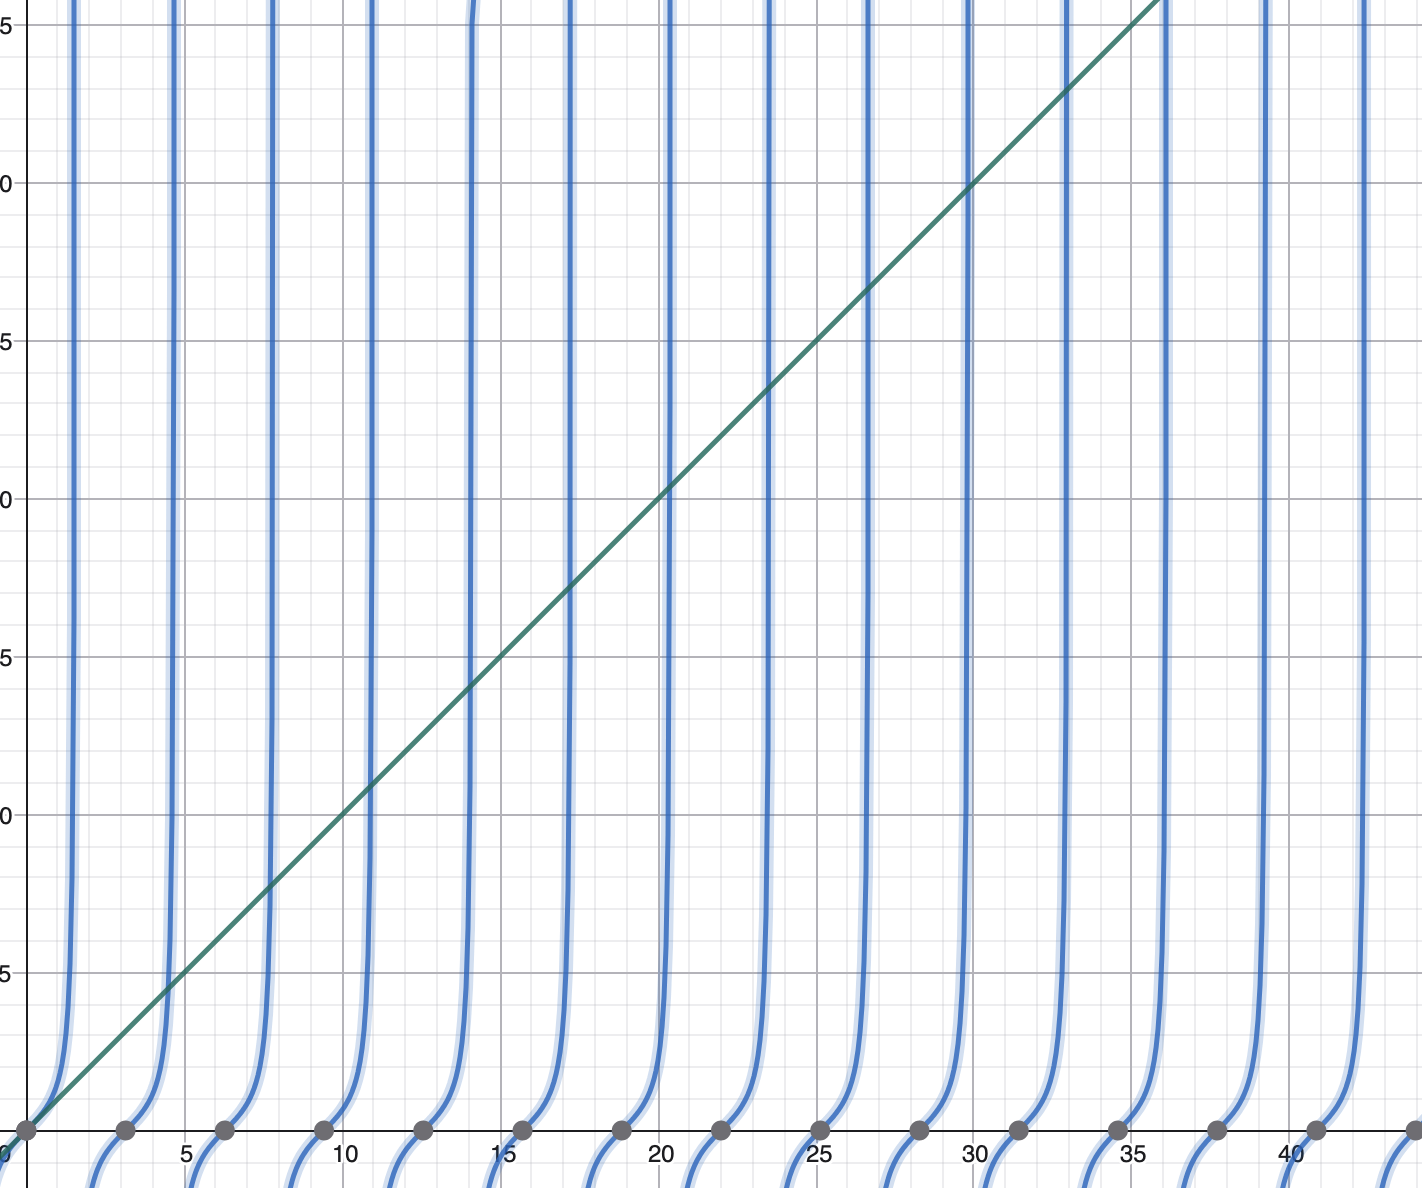
\includegraphics[width=0.8\textwidth,valign=t]{fig/prob4.10.png}
    
    For large $N,$ the solution is approximately located at 
    $(2N+\frac{1}{2})\pi.$

    $$
    ka = (2N+\frac{1}{2})\pi\Rightarrow
    \frac{\sqrt{2mE}}{\hbar}a=(2N+\frac{1}{2})\pi
    \Rightarrow 
    E = \frac{\hbar^2\pi^2}{2ma^2}(2N+\frac{1}{2})
    $$
    
\end{enumerate}

\subsection*{Sol. 11}
For $l=0,$ the differential equation is
$$
u'' = \frac{-2m(E-V)}{\hbar^2}u
$$

For $0<r<a,$
$$
u= A\sin k r,
$$
where $k=\frac{\sqrt{2m(E+V_0)}}{\hbar}.$
For $r>a,$
$$
u=Be^{-\frac{\sqrt{-2mE}}{\hbar}r}.
$$

The continuity condition requires 
$$
A\sin ka = Be^{-\frac{\sqrt{-2mE}}{\hbar}a}
$$
$$
kA\cos ka = -\frac{\sqrt{-2mE}}{\hbar}Be^{-\frac{\sqrt{-2mE}}{\hbar}a}
$$
Divide both equations give
$$
k\cot ka = -\frac{\sqrt{-2mE}}{\hbar}
\Rightarrow
\cot ka = -\sqrt{\frac{-E}{E+V_0}} 
=-\sqrt{\frac{V_0-\frac{k^2\hbar^2}{2m}}{\frac{k^2\hbar^2}{2m}}}
$$
$$
\cot z = -\sqrt{\frac{\frac{a^2V_02m}{\hbar^2}-z^2}{z^2}}
=-\sqrt{\frac{z_0^2}{z^2}-1},
$$
where $z = ka,$ $z_0 = \frac{a\sqrt{2mV_0}}{\hbar}.$ The ground state is thus the smallest positive $z$ that solves this transcendental equation.
 Note that the right hand side has zero at 
 $
 z=z_0,
 $
 so when $z_0<\frac{\pi}{2}\Rightarrow V_0<\frac{\pi^2\hbar^2}{8ma^2},$ there is no allowed bound state.

 \subsection*{Sol. 12}
 For $R_{30},$
 $$
 c_1 = \frac{2(0+0+1-3)}{(0+1)(0+2\cdot 0+2)}c_0
 =-2c_0
 $$
 $$
 c_2 = \frac{2(1+0+1-3)}{(1+1)(1+2\cdot 0+2)}c_1
 =\frac{-1}{3}c_1
 =\frac{2}{3}c_0
 $$
 $$
 c_3 = \frac{2(2+0+1-3)}{(2+1)(2+2\cdot 0+2)}c_2
 =0
 $$

 $$
 R_{30}(r)=
 \frac{1}{r}
 \frac{r}{3a} 
 e^{-\frac{r}{3a}}
 \left(\frac{2}{3}\left(\frac{r}{3a}\right)^2-2\frac{r}{3a}+1\right)c_0
 $$

 $$
 c_1 = \frac{2(0+1+1-3)}{(0+1)(0+2\cdot 1+2)}c_0
 =-\frac{1}{2}c_0
 $$
 $$
 c_2 = \frac{2(1+1+1-3)}{(1+1)(1+2\cdot 1+2)}c_1
 =0
 $$


 $$
 R_{31}(r)=
 \frac{1}{r}
 \left(\frac{r}{3a}\right)^2 
 e^{-\frac{r}{3a}}
 \left(-\frac{1}{2}\frac{r}{3a}+1\right)c_0
 $$

 $$
 c_1 = \frac{2(0+2+1-3)}{(0+1)(0+2\cdot 1+2)}c_0
 =0
 $$



 $$
 R_{32}(r)=
 \frac{1}{r}
 \left(\frac{r}{3a}\right)^3 
 e^{-\frac{r}{3a}}
 c_0
 $$

  \subsection*{Sol. 13}
  \begin{enumerate}
      \item 
      \begin{align*}
          \int_0^\infty 
          \frac{c_0^2}{4a^2}
          \left(
          1-\frac{r}{2a}
          \right)^2
          e^{-r/a}
          r^2dr=\frac{ac_0^2}{2}
          \Rightarrow c_0=\sqrt{\frac{2}{a}}
      \end{align*}
      \begin{align*}
          \psi_{200}(r,\theta,\phi)
          =
          \sqrt{\frac{2}{a}}
          \frac{1}{2a}
          \left(1-\frac{r}{2a}\right)
          e^{-r/2a}
          \sqrt{\frac{1}{4\pi}}
      \end{align*}

      \begin{align*}
          \int_0^\infty 
          \frac{c_0^2}{16a^4}
          r^2
          e^{-r/a}
          r^2dr=\frac{3ac_0^2}{2}
          \Rightarrow c_0=\sqrt{\frac{2}{3a}}
      \end{align*}
      \item 
      \begin{align*}
          \psi_{211}(r,\theta,\phi)
          =
          -\sqrt{\frac{2}{3a}}
          \frac{1}{4a^2}
          r
          e^{-r/2a}
          \sqrt{\frac{3}{8\pi}}
          \sin\theta e^{i\phi}
      \end{align*}
        \begin{align*}
          \psi_{210}(r,\theta,\phi)
          =
          \sqrt{\frac{2}{3a}}
          \frac{1}{4a^2}
          r
          e^{-r/2a}
          \sqrt{\frac{1}{4\pi}}
      \end{align*}
      \begin{align*}
          \psi_{21-1}(r,\theta,\phi)
          =\sqrt{\frac{2}{3a}}
          \frac{1}{4a^2}
          r
          e^{-r/2a}
          \sqrt{\frac{3}{8\pi}}
          \sin\theta 
          e^{-i\phi}
      \end{align*}
  \end{enumerate}

  \subsection*{Sol. 14}
  \begin{enumerate}
      \item 
      \begin{align*}
          L_0(x) = 1
      \end{align*}
      \begin{align*}
          L_1(x) = 
          \frac{e^x}{1}
          \frac{d}{dx}
          (e^{-x}x)
          =
          1-x
      \end{align*}
       \begin{align*}
          L_2(x) = 
          \frac{e^x}{2}
          \frac{d^2}{dx^2}
          (e^{-x}x^2)
          =
          \frac{1}{2}x^2
          -2x + 1
      \end{align*}
      \begin{align*}
          L_3(x) = 
          \frac{e^x}{6}
          \frac{d^3}{dx^3}
          (e^{-x}x^3)
          =
          -\frac{1}{6}
          x^3 
          +\frac{3}{2}x^2 
          -3x 
          + 1
      \end{align*}
      \item 
      $$
      v(\rho)
      =L^{2\cdot 2+1}_{5-2-1}
      (2\rho)
      =L^5_2(2\rho)
      $$
      $$
      L^5_2(x)
      =(-1)^5
      \frac{d^5}{dx^5}
      L_7(x)
      $$
      $$
      L_7(x)=
     \frac{e^x}{7!}
     \frac{d^7}{dx^7}
     (e^{-x}x^7)
     =
     -\frac{1}{7!}
     (x^7-49x^6+882x^5
     -7350x^4+29400x^3-52920x^2+35280x-5040)
      $$
      \begin{align*}
          L^5_2(x)
    =& \frac{1}{7!}
    (2520x^2-35280x+105840)\\
    =&
    \frac{1}{2}x^2-7x+21
      \end{align*}
      Therefore
      $$
      v(\rho)
      =2\rho^2-14\rho+21
      $$
      \item 
      $$
      c_1 = \frac{2(0+2+1-5)}{(0+1)(0+4+2)}c_0 = -\frac{2}{3}c_0
      $$
      $$
      c_2 = \frac{2(1+2+1-5)}
      {(1+1)(1+4+2)}c_1 = -\frac{1}{7}c_1=
      \frac{2}{21}c_0
      $$
      $$
      c_3 = \frac{2(2+2+1-5)}
      {(2+1)(2+4+2)}c_1 = 0
      $$
      Therefore 
      $$
      v(\rho)
      =(\frac{2}{21}\rho^2-\frac{2}{3}\rho+1)c_0
      $$
      
  \end{enumerate}

    \subsection*{Sol. 15}
    \begin{enumerate}
        \item 
        \begin{align*}
            \langle r\rangle
            =\int_0^\infty 
            \int_0^\pi 
            \int_0^{2\pi}
            r
            \frac{1}{\pi a^3}
            e^{-2r/a}
            r^2\sin\theta
            drd\theta d\phi
            =\frac{3a}{2}
        \end{align*}
        \begin{align*}
            \langle r^2\rangle
            =\int_0^\infty 
            \int_0^\pi 
            \int_0^{2\pi}
            r^2
            \frac{1}{\pi a^3}
            e^{-2r/a}
            r^2\sin\theta
            drd\theta d\phi
            =3a^2
        \end{align*}
        \item 
        $$
        \langle x\rangle = 0
        $$
        $$
        \langle x^2\rangle = a^2
        $$
        \item 
        $$
        \psi_{211}(r,\theta,\phi)
          =
          -\sqrt{\frac{2}{3a}}
          \frac{1}{4a^2}
          r
          e^{-r/2a}
          \sqrt{\frac{3}{8\pi}}
          \sin\theta e^{i\phi}
        $$

        \begin{align*}
            \langle x^2\rangle
            =&
            \int_0^\infty 
            \int_0^\pi 
            \int_0^{2\pi}
            r^2\sin^2\theta\cos^2\phi 
            \frac{2}{3a}
            \frac{1}{16a^4}
            r^2
            e^{-r/a}
            \frac{3}{8\pi}
            \sin^2(\theta )
            r^2\sin\theta 
            drd\theta d\phi\\
            =&12a^2
        \end{align*}
    \end{enumerate}

    \subsection*{Sol. 16}
    The probability density along the radial of the ground state is 
    $$
    \int_0^{2\pi}
    \int_0^{\pi}
    \frac{1}{\pi a^3}
            e^{-2r/a}
            r^2\sin\theta
            d\theta d\phi
            =
            \frac{4}{ a^3}
            e^{-2r/a}
            r^2,
    $$
    which attain the maximum at 
    $
    r=a.
    $

    \subsection*{Sol. 17}
    Note that $$
    [z,[H,z]] = 2zHz-z^2H-Hz^2.
    $$
    Also note that 
    \begin{align*}
    [H,z]=&\frac{1}{2m}([p^2_z, z])\\
    =&\frac{1}{2m}(p_z[p_z,z]+[p_z,z]p_z)\\
    =&\frac{-i\hbar p_z}{m}
    \end{align*}
    $$
    [z,[H,z]]
    =[z, \frac{-i\hbar p_z}{m}]
    =\frac{\hbar^2}{m}.
    $$
    Therefore
    $$
    \frac{\hbar^2}{m}
    =2\langle zHz\rangle
    -\langle z^2H\rangle
    -\langle Hz^2\rangle
    =2\langle zHz\rangle
    -2a^2E_1,
    $$
    $$
    \langle zHz\rangle
    =\frac{\hbar^2}{2m}+a^2E_1.
    $$


    \subsection*{Sol. 18}
    \begin{enumerate}
        \item 
        \begin{align*}
            \Psi(\bm{r},t)
            =&
            \frac{1}{\sqrt{2}}
            \left(
            \sqrt{\frac{2}{3a}}
            \frac{1}{4a^2}
            re^{-r/2a}
            \sqrt{\frac{3}{8\pi}}
            \sin\theta 
            (-e^{i\phi}+e^{-i\phi})
            \right)e^{-iE_2t/\hbar}\\
            =&
            \frac{-i}{2a^2}
            \sqrt{\frac{1}{8\pi a}}
            re^{-r/2a}
            \sin\theta 
            \sin\phi
            e^{-iE_2t/\hbar}
        \end{align*}
        \item 
        \begin{align*}
            \langle V\rangle
            =&
            -\frac{e^2}{4\pi\epsilon_0}
            \int_0^\infty 
            \int_0^\pi 
            \int_0^{2\pi}
            \frac{1}{r}
            \frac{1}{4a^4}
            \frac{1}{8\pi a}
            r^2e^{-r/a}
            \sin^2\theta 
            \sin^2\phi
            r^2\sin\theta drd\theta d\phi\\
            =&\frac{-e^2}{16\pi\epsilon_0a}\approx -6.8028eV
        \end{align*}
    \end{enumerate}

    \subsection*{Sol. 19}

    $$
    E_n(Z)
    =-\left[\frac{m_e}{2\hbar^2}
    \left(
    \frac{Ze^2}{4\pi\epsilon_0}
    \right)^2
    \right] 
    \frac{1}{n^2}
    $$

    $$
    E_1(Z)
    =-\left[\frac{m_e}{2\hbar^2}
    \left(
    \frac{Ze^2}{4\pi\epsilon_0}
    \right)^2
    \right] 
    $$

    $$
    a(Z)
    =\frac{4\pi\epsilon_0\hbar^2}{m_eZe^2}
    $$

    $$\mathcal{R}(Z)
    =\frac{m_e}{4\pi c\hbar^3}
    \left(
    \frac{Ze^2}{4\pi\epsilon_0}
    \right)^2
    $$


    \subsection*{Sol. 20}
    \begin{enumerate}
        \item 
        $$
        V(r)=\frac{-GMm_e}{r}
        $$
        \item By changing $\frac{e^2}{4\pi\epsilon_0}$ to $GMm_e,$
        $$
        a_g = \frac{\hbar^2}{GMm_e^2}
        $$
        The actual number
        is about $2.349
        \times 10^{-138}m.$
        \item 
        $$
        E_n = 
        -\left[
        \frac{m_e}{2\hbar^2}
        G^2M^2m_e^2
        \right]\frac{1}{n^2}
        $$
        $$
        -\left[
        \frac{m_e}{2\hbar^2}
        G^2M^2m_e^2
        \right]\frac{1}{n^2}
        =-\frac{GMm_e}{2r_0}
        \Rightarrow n = \sqrt{\frac{r_0}{a_g}}
        $$

        $r_0\approx 1.496\times10^{11}m,$
        so $n\approx 2.52\times10^{74}.$
        \item 
        From level $n$ to $n-1,$ the energy will release
        $$
        \frac{m_e}{2\hbar^2}G^2M^2m_e^2
        \frac{2n-1}{(n-1)^2n^2}
        \approx
        \frac{GMm_e}{a_gn^3}
        $$
        About $2.1\times10^{-41}J,$
        the corresponding wavelength is 
        $9.459\times 10^{15}m,$ just approximately a light year.
    \end{enumerate}

   \subsection*{Sol. 21}
   \begin{align*}
        \hbar^2 l(l+1)
       =&\langle f^{m}_l, L^2f^m_l\rangle\\
       =&
       \langle f^{m}_l, L_-L_+f^m_l\rangle
       +\langle f^{m}_l, L_z^2f^m_l\rangle
       +\hbar \langle f^{m}_l, L_zf^m_l\rangle\\
       =&(A^m_l)^2 + \hbar^2m^2 + \hbar^2 m\\
   \end{align*}
   $$
   A^m_l = \hbar\sqrt{l(l+1)-m(m+1)}
   =\hbar\sqrt{(l-m)(l+m+1)}
   $$
   \begin{align*}
        \hbar^2 l(l+1)
       =&\langle f^{m}_l, L^2f^m_l\rangle\\
       =&
       \langle f^{m}_l, L_+L_-f^m_l\rangle
       +\langle f^{m}_l, L_z^2f^m_l\rangle
       -\hbar \langle f^{m}_l, L_zf^m_l\rangle\\
       =&(B^m_l)^2 + \hbar^2m^2 - \hbar^2 m\\
   \end{align*}
   $$
   B^m_l = \hbar\sqrt{l(l+1)-m(m-1)}
   =\hbar\sqrt{(l+m)(l-m+1)}
   $$

   \subsection*{Sol. 22}
   \begin{enumerate}
       \item 
       $L_z=xp_y-yp_x,$
   so 
   $$
   [L_z, x]=i\hbar y,\;
   [L_z, y]=-i\hbar x,\;
   [L_z, z]=0\;
   $$
   $$
   [L_z, p_x]=i\hbar p_y,\;
   [L_z, p_y]=-i\hbar p_x,\;
   [L_z, p_z]=0\;
   $$
   \item 
   $$
   [L_z,L_x]
   =[L_z, yp_z-zp_y]
   =-i\hbar xp_z
   +i\hbar zp_x
   =i\hbar L_y
   $$
   \item 
   \begin{align*}
   [L_z, r^2]
   =&
   [L_z, x^2] + 
   [L_z, y^2] + 
   [L_z, z^2]\\
   =&x[L_z, x] + [L_z,x]x+
   y[L_z, y] + [L_z,y]y+
   z[L_z, z] + [L_z,z]z\\
   =&i\hbar xy+
   i\hbar yx
   -i\hbar yx 
   -i\hbar xy  = 0
   \end{align*}
   \begin{align*}
   [L_z, p^2]
   =&
   [L_z, p_x^2] + 
   [L_z, p_y^2] + 
   [L_z, p_z^2]\\
   =&p_x[L_z, p_x] + [L_z,p_x]p_x+
   p_y[L_z, p_y] + [L_z,p_y]p_y+
   p_z[L_z, p_z] + [L_z,p_z]p_z\\
   =&i\hbar p_xp_y+
   i\hbar p_yp_x
   -i\hbar p_yp_x 
   -i\hbar p_xp_y  = 0
   \end{align*}
   \item 
   \begin{align*}
       [L_z, r] =& [xp_y - yp_x, r]\\
       =&x[p_y,r]-y[p_x,r]\\
       =&-i\hbar x\frac{y}{r} +i\hbar \frac{x}{r} = 0.
   \end{align*}
   Expand $V$ in Taylor series, we then obtain that $L_z$ commutes with $H,$ and therefore all three components of the angular momentum commute with $H.$
   
   \end{enumerate}


   \subsection*{Sol. 23}
   \begin{enumerate}
       \item 
       Note that 
   \begin{align*}
   [V, L_x] = &
   [V, yp_z-zp_y]\\
   =&[V, yp_z] - [V,zp_y]\\
   =&y[V,p_z] + [V,y]p_z - z[V,p_y]-[V,z]p_y\\
   =&i\hbar yV_z- i\hbar zV_y,
   \end{align*}
   similarly 
   $$
   [V, L_y]=i\hbar(zV_y-yV_z),
   $$
   $$
   [V, L_z]=i\hbar(xV_y-yV_x).
   $$
   \begin{align*}
       \frac{d}{dt}\langle \bm{L}\rangle
       =&\frac{i}{\hbar}
       \langle [H, \bm{L}]\rangle\\
       =&\frac{i}{\hbar}\langle[V, (L_x, L_y, L_z)]\rangle\\
       =&-\langle(yV_z-zV_y, -xV_z+zV_x, xV_y-yV_x)\rangle
   \end{align*}
   \begin{align*}
       \bm{r}\times (-\nabla V)
       =-(yV_z-zV_y, -xV_z+zV_x, xV_y-yV_x).
   \end{align*}
   Hence 
   $$
   \frac{d}{dt}\langle\bm{L}\rangle
   =\langle \bm{N}\rangle.
   $$
   \item 
   In spherical coordinate, $$\nabla V=V_r\hat{r},$$ so the cross product with $\bm{r}=r\hat{r}$ cancels.
   \end{enumerate}

   \subsection*{Sol. 24}
\begin{enumerate}
    \item 
    \begin{align*}
        L_+L_-f
        =&-\hbar 
        e^{i\phi}
        \left(
        \frac{\partial}{\partial\theta}
        +i\cot\theta  
        \frac{\partial}{\partial\phi}
        \right)
        \hbar 
        e^{-i\phi}
        \left(
        \frac{\partial}{\partial\theta}
        -
        i\cot\theta  
        \frac{\partial}{\partial\phi}
        \right)f\\
        =&-\hbar^2 
        e^{i\phi}
        \left(
        \frac{\partial}{\partial\theta}
        +i\cot\theta  
        \frac{\partial}{\partial\phi}
        \right)
        e^{-i\phi}
        (f_\theta
        -i\cot\theta f_\phi)\\
        =&
        -\hbar^2
        e^{i\phi}
        (e^{-i\phi}f_{\theta\theta} 
        -ie^{-i\phi}(-\csc^2\theta f_\phi + \cot\theta f_{\phi\theta})\\
        &+i\cot\theta
        (-ie^{-i\phi}f_\theta + 
        e^{-i\phi}f_{\theta\phi})
        +\cot^2\theta(-ie^{-i\phi}f_\phi + e^{-i\phi}f_{\phi\phi})
        )\\
        =&-\hbar^2(
        f_{\theta\theta}
        +
        if_\phi 
        +\cot\theta f_{\theta}
        +\cot^2\theta f_{\phi\phi}
        ).
    \end{align*}    
    $$
    L_+L_- = 
    -\hbar^2
    \left(
    \frac{\partial^2}{\partial\theta^2 }
    +\cot\theta
    \frac{\partial}{\partial\theta}
    +\cot^2\theta
    \frac{\partial^2}{\partial\phi^2}
    +i\frac{\partial}{\partial\phi}
    \right)
    $$
    \item 
    \begin{align*}
        L^2=&L_+L_-+L_z^2 -\hbar L_z\\
        =&
        -\hbar^2
    \left(
    \frac{\partial^2}{\partial\theta^2 }
    +\cot\theta
    \frac{\partial}{\partial\theta}
    +\cot^2\theta
    \frac{\partial^2}{\partial\phi^2}
    +i\frac{\partial}{\partial\phi}
    \right)
    -\hbar^2\frac{\partial^2}{\partial\phi^2}
    +i\hbar^2\frac{\partial}{\partial\phi}\\
    =&-\hbar^2\left(
    \frac{\partial^2}{\partial\theta^2 }
    +\cot\theta
    \frac{\partial}{\partial\theta}
    -\csc^2\theta
    \frac{\partial^2}{\partial\phi^2}
    \right)
    \end{align*}
    
\end{enumerate}

   \subsection*{Sol. 25}
   \begin{enumerate}
       \item $$
       L_+Y^l_l = 0
       $$
       \item 
       $$
       \hbar e^{i\phi}
       (\frac{\partial}{\partial\theta}+i\cot\theta\frac{\partial}{\partial\phi})Y^l_l = 0
       $$
       Also, 
       $$
       -i\hbar\frac{\partial}{\partial\phi} Y^l_l = \hbar lY^l_l
       \Rightarrow 
       Y^l_l = A(\theta)e^{il\phi}.
       $$
       $$
       \frac{\partial}{\partial\theta}
       Y^l_l 
       -\cot\theta lY^l_l = 0
       $$
       $$
       A(\theta)= C\sin^l\theta,
       $$
       so 
       $$
       Y^l_l = C\sin^l\theta e^{il\phi}.
       $$
       \item 
       Let $I_{2l+1} = \int_0^{\pi}\sin^{2l+1}\theta d\theta,$
       then 
       \begin{align*}
           I_{2l+1} =&  \int_0^{\pi}\sin^{2l+1}\theta d\theta\\
           =&-\sin^{2l}\theta \cos\theta 
           \bigg|_0^\pi 
           +2l\int\sin^{2l-1}\theta \cos^2\theta d\theta \\
           =&2l(I_{2l-1} - I_{2l+1})
       \end{align*}
       \begin{align*}
      I_{2l+1} =& \frac{2l}{2l+1}I_{2l-1}\\
      =&\frac{2l}{2l+1}\frac{2l-2}{2l-1}I_{2l-3}\\
      =&\frac{2l}{2l+1}\frac{2l-2}{2l-1}\dots \frac{2}{3}I_1\\
      =&\frac{2^{2l}(l!)^22}{(2l+1)!}
       \end{align*}

       \begin{align*}
           \int_0^{2\pi}
           \int_0^\pi
           C^2\sin^{2l}\theta 
           \sin\theta d\theta d\phi
           =&C^22\pi\frac{2^{2l}(l!)^22}{(2l+1)!}
           \Rightarrow 
           C = (-1)^l\sqrt{\frac{(2l+1)!}{\pi}}
           \frac{1}{2^{l+1}l!}
       \end{align*}
      
   \end{enumerate}
   \subsection*{Sol. 26}
   \begin{align*}
       L_+Y^{1}_2 =& -\sqrt{\frac{15}{8\pi}}
       \hbar e^{i\phi}
       \left(\frac{\partial}{\partial\theta}
       +i\cot\theta 
       \frac{\partial}{\partial\phi}\right)
       \sin\theta \cos\theta e^{i\phi}\\
       =&
       -\sqrt{\frac{15}{8\pi}}
       \hbar e^{i\phi}
       [(\cos^2\theta -\sin^2\theta)e^{i\phi}
       +i\cot\theta 
       \sin\theta \cos\theta ie^{i\phi}
       ]\\
       =&
       \sqrt{\frac{15}{8\pi}}
       \hbar e^{2i\phi}
       \sin^2\theta 
   \end{align*}
   By 4.121, 
   $$
   A^1_2 = 
   2\hbar,
   $$
   so 
   $$
    Y^2_2
    =\sqrt{\frac{15}{32\pi}}
    e^{2i\phi}
    \sin^2\theta.
   $$

   \subsection*{Sol. 27}
   \begin{enumerate}
       \item 
       Let $\omega$ be the angular speed, 
       $r_1=\frac{m_2a}{m_1+m_2},$ 
       $p_1 = \frac{m_1m_2a}{m_1+m_2}\omega,$
       $r_2=\frac{m_1a}{m_1+m_2},$ 
       $p_2 = \frac{m_1m_2a}{m_1+m_2}\omega$
       \begin{align*}
           L = &
       \frac{m_2a}{m_1+m_2}
       \frac{m_1m_2a}{m_1+m_2}\omega+
       \frac{m_1a}{m_1+m_2}\frac{m_1m_2a}{m_1+m_2}\omega\\
       =&\frac{m_1m_2a^2}{m_1+m_2}\omega = I\omega,
       \end{align*}
       where $I=\frac{m_1m_2}{m_1+m_2}a^2.$

       The energy is 
       \begin{align*}
           E =& \frac{p_1^2}{2m_1}
           +\frac{p_2^2}{2m_2}\\
           =&
           \left(\frac{m_1m_2a}{m_1+m_2}\omega\right)^2
           \frac{m_1+m_2}{2m_1m_2}\\
           =&\frac{1}{2}I\omega^2      \\
           =&\frac{L^2}{2I}.
       \end{align*}
       By the theory developed above, the allowed eigenvalues of $L^2$ are $\hbar n(n+1),$ for $n=0,1,\dots.$ Therefore, the allowed energies of this rigid rotor are $$
       E_n = \frac{\hbar^2}{2I}n(n+1).
       $$
       \item The Hamiltonian is $\frac{L^2}{2I},$ so the normalized eigenfunctions are the spherical harmonics. For the energy level $n,$ there are $2n+1$ possible $m$ values.
       \item 
       The difference between two adjacent energy level is 
       $$
       E_{n+1}
       -E_n
       =\frac{\hbar^2}{I}
       (n+1).
       $$
       Any energy differences is therefore 
       $\frac{\hbar^2j}{I},$ for $j=1,2,3\dots.$
       $$
       \nu_j=\frac{\hbar^2j}{I}\frac{1}{2\pi\hbar}
       =\frac{\hbar j}{2\pi I}.
       $$
       \item 
       The frequency separation is $\frac{\hbar}{2\pi I}.$
       From the figure, the frequency separation is approximately 
       $1.2\times10^{11}Hz.$
       $$
       a = \sqrt{\frac{\hbar}{2\pi\Delta\nu}\frac{m_1+m_2}{m_1m_2}}\approx 1.108\times 10^{-10}m.
       $$
   \end{enumerate}
   \subsection*{Sol. 28}
   Assume the angular speed is $\omega.$
   \begin{align*}
       \frac{1}{2}\hbar = 
       &\int_0^{2\pi}\int_{0}^\pi\int_0^{r_c} 
       r^2\sin^2\theta\omega
       \rho
       r^2\sin\theta drd\theta d\phi\\
       =&\frac{8\pi r_c^5}{15}\omega 
       \frac{m}{\frac{4}{3}\pi r_c^3}\\
       =&\frac{2r_c^2\omega m}{5}
   \end{align*}
   The point at the equator moves at speed
   $$
   v = r_c\omega = 
   \frac{\hbar}{2}
   \frac{5}{2r_c m}
   =\frac{5\hbar\pi\epsilon_0c^2}{e^2}\approx 5.14\times 10^{10}m/s.
   $$
   \subsection*{Sol. 29}
\begin{enumerate}
    \item 
    \begin{align*}
        S_xS_y 
        -S_yS_x
    =&
    \frac{\hbar^2}{4}
    \begin{pmatrix}
    0 & 1 \\
    1 & 0
    \end{pmatrix}
    \begin{pmatrix}
    0 & -i \\
    i & 0
    \end{pmatrix}
    -
    \frac{\hbar^2}{4}
    \begin{pmatrix}
    0 & -i \\
    i & 0
    \end{pmatrix}
    \begin{pmatrix}
    0 & 1 \\
    1 & 0
    \end{pmatrix}\\
    =&
    \frac{\hbar^2}{4}
    \begin{pmatrix}
        i & 0\\
        0 & -i
    \end{pmatrix}
    -
    \frac{\hbar^2}{4}
    \begin{pmatrix}
        -i & 0\\
        0 & i
    \end{pmatrix}
    \\
    =&
    \frac{\hbar^2}{4}
    \begin{pmatrix}
        2i & 0\\
        0 & -2i
    \end{pmatrix}\\
    =&i\hbar S_z
    \end{align*}

    \begin{align*}
        S_yS_z 
        -S_zS_y
    =&
    \frac{\hbar^2}{4}
    \begin{pmatrix}
    0 & -i \\
    i & 0
    \end{pmatrix}
    \begin{pmatrix}
    1 & 0 \\
    0 & -1
    \end{pmatrix}
    -
    \frac{\hbar^2}{4}
    \begin{pmatrix}
    1 & 0 \\
    0 & -1
    \end{pmatrix}
    \begin{pmatrix}
    0 & -i \\
    i & 0
    \end{pmatrix}\\
    =&
    \frac{\hbar^2}{4}
    \begin{pmatrix}
        0 & i\\
        i & 0
    \end{pmatrix}
    -
    \frac{\hbar^2}{4}
    \begin{pmatrix}
        0 & -i\\
        -i & 0
    \end{pmatrix}
    \\
    =&
    \frac{\hbar^2}{4}
    \begin{pmatrix}
        0 & 2i\\
        2i & 0
    \end{pmatrix}\\
    =&i\hbar S_x
    \end{align*}

    \begin{align*}
        S_zS_x
        -S_xS_z
    =&
    \frac{\hbar^2}{4}
    \begin{pmatrix}
    1 & 0 \\
    0 & -1
    \end{pmatrix}
    \begin{pmatrix}
    0 & 1 \\
    1 & 0
    \end{pmatrix}
    -
    \frac{\hbar^2}{4}
    \begin{pmatrix}
    0 & 1 \\
    1 & 0
    \end{pmatrix}
    \begin{pmatrix}
    1 & 0 \\
    0 & -1
    \end{pmatrix}\\
    =&
    \frac{\hbar^2}{4}
    \begin{pmatrix}
        0 & 1\\
        -1 & 0
    \end{pmatrix}
    -
    \frac{\hbar^2}{4}
    \begin{pmatrix}
        0 & -1\\
        1 & 0
    \end{pmatrix}
    \\
    =&
    \frac{\hbar^2}{4}
    \begin{pmatrix}
        0 & 2\\
        -2 & 0
    \end{pmatrix}\\
    =&i\hbar S_y
    \end{align*}
    \item 
    $$
    \sigma_x\sigma_x = 
    \begin{pmatrix}
        0 & 1\\
        1 & 0
    \end{pmatrix}
    \begin{pmatrix}
        0 & 1\\
        1 & 0
    \end{pmatrix}
    =\begin{pmatrix}
        1 & 0\\
        0 & 1
    \end{pmatrix}
    =I
    $$
    
    $$
    \sigma_x\sigma_y = 
    \begin{pmatrix}
        0 & 1\\
        1 & 0
    \end{pmatrix}
    \begin{pmatrix}
        0 & -i\\
        i & 0
    \end{pmatrix}
    =\begin{pmatrix}
        i & 0\\
        0 & -i
    \end{pmatrix}
    =i\sigma_z
    $$

    $$
    \sigma_x\sigma_z = 
    \begin{pmatrix}
        0 & 1\\
        1 & 0
    \end{pmatrix}
    \begin{pmatrix}
        1 & 0\\
        0 & -1
    \end{pmatrix}
    =\begin{pmatrix}
        0 & -1\\
        1 & 0
    \end{pmatrix}
    =-i\sigma_y
    $$



    $$
    \sigma_y\sigma_x = 
    \begin{pmatrix}
        0 & -i\\
        i & 0
    \end{pmatrix}
    \begin{pmatrix}
        0 & 1\\
        1 & 0
    \end{pmatrix}
    =\begin{pmatrix}
        -i & 0\\
        0 & i
    \end{pmatrix}
    =-i\sigma_z
    $$
    
    $$
    \sigma_y\sigma_y = 
    \begin{pmatrix}
        0 & -i\\
        i & 0
    \end{pmatrix}
    \begin{pmatrix}
        0 & -i\\
        i & 0
    \end{pmatrix}
    =\begin{pmatrix}
        1 & 0\\
        0 & 1
    \end{pmatrix}
    =I
    $$

    $$
    \sigma_y\sigma_z = 
    \begin{pmatrix}
        0 & -i\\
        i & 0
    \end{pmatrix}
    \begin{pmatrix}
        1 & 0\\
        0 & -1
    \end{pmatrix}
    =\begin{pmatrix}
        0 & i\\
        i & 0
    \end{pmatrix}
    =i\sigma_x
    $$
    %%%%

    $$
    \sigma_z\sigma_x = 
    \begin{pmatrix}
        1 & 0\\
        0 & -1
    \end{pmatrix}
    \begin{pmatrix}
        0 & 1\\
        1 & 0
    \end{pmatrix}
    =\begin{pmatrix}
        0 & 1\\
        -1 & 0
    \end{pmatrix}
    =i\sigma_y
    $$
    
    $$
    \sigma_z\sigma_y = 
    \begin{pmatrix}
        1 & 0\\
        0 & -1
    \end{pmatrix}
    \begin{pmatrix}
        0 & -i\\
        i & 0
    \end{pmatrix}
    =\begin{pmatrix}
        0 & -i\\
        -i & 0
    \end{pmatrix}
    =-i\sigma_x
    $$

    $$
    \sigma_z\sigma_z = 
    \begin{pmatrix}
        1 & 0\\
        0 & -1
    \end{pmatrix}
    \begin{pmatrix}
        1 & 0\\
        0 & -1
    \end{pmatrix}
    =I
    $$
    
\end{enumerate}

   \subsection*{Sol. 30}
   \begin{enumerate}
       \item $\frac{1}{5}$
       \item 
       \begin{align*}
           \langle S_x\rangle
           =&\frac{1}{25}
           \frac{\hbar}{2}
           \begin{pmatrix}
               -3i & 4
           \end{pmatrix}
           \begin{pmatrix}
               0 & 1 \\
               1 & 0
           \end{pmatrix}
           \begin{pmatrix}
               3i\\4
           \end{pmatrix}\\
           =& \frac{\hbar}{50}
           \begin{pmatrix}
               -3i & 4
           \end{pmatrix}
           \begin{pmatrix}
               4 \\ 3i
           \end{pmatrix}\\
           =&0
       \end{align*}
       \begin{align*}
           \langle S_y\rangle
           =&\frac{1}{25}
           \frac{\hbar}{2}
           \begin{pmatrix}
               -3i & 4
           \end{pmatrix}
           \begin{pmatrix}
               0 & -i \\
               i & 0
           \end{pmatrix}
           \begin{pmatrix}
               3i\\4
           \end{pmatrix}\\
           =& \frac{\hbar}{50}
           \begin{pmatrix}
               -3i & 4
           \end{pmatrix}
           \begin{pmatrix}
               -4i \\ -3
           \end{pmatrix}\\
           =&\frac{-12\hbar}{25}
       \end{align*}
       \begin{align*}
           \langle S_z\rangle
           =&\frac{1}{25}
           \frac{\hbar}{2}
           \begin{pmatrix}
               -3i & 4
           \end{pmatrix}
           \begin{pmatrix}
               1 & 0 \\
               0 & -1
           \end{pmatrix}
           \begin{pmatrix}
               3i\\4
           \end{pmatrix}\\
           =& \frac{\hbar}{50}
           \begin{pmatrix}
               -3i & 4
           \end{pmatrix}
           \begin{pmatrix}
               3i \\ -4
           \end{pmatrix}\\
           =&\frac{-7\hbar}{50}
       \end{align*}
       \item 

        \begin{align*}
           \langle S^2_x\rangle
           =
           \langle S^2_y\rangle
           =
           \langle S^2_z\rangle
           =
           \frac{\hbar^2}{4}
       \end{align*}

       $$
       \sigma_{S_x}
       =\frac{\hbar}{2},\;
       \sigma_{S_y}
       =\frac{7\hbar}{50},\;
       \sigma_{S_z}
       =\frac{12\hbar}{25}
       $$
       \item 
       $$
       \sigma_{S_x}\sigma_{S_y}
       =\frac{7\hbar^2}{100}\geq 
       \frac{\hbar}{2}\frac{7\hbar}{50}=|\langle S_z\rangle|
       $$
       $$
       \sigma_{S_x}\sigma_{S_z}
       =\frac{6\hbar^2}{25}\geq 
       \frac{\hbar}{2}\frac{12\hbar}{25}=|\langle S_y\rangle|
       $$
       $$
       \sigma_{S_y}\sigma_{S_z}
       =\frac{42\hbar^2}{625}\geq 
       0=|\langle S_x\rangle|
       $$
   \end{enumerate}

   \subsection*{Sol. 31}
   \begin{align*}
       \langle S_x\rangle =& 
       \frac{\hbar}{2}
       \begin{pmatrix}
           \bar a & \bar b
       \end{pmatrix}
       \begin{pmatrix}
           0 & 1 \\
           1 & 0
       \end{pmatrix}
       \begin{pmatrix}
           a \\ b 
       \end{pmatrix}\\
       =&
       \frac{\hbar}{2}
        \begin{pmatrix}
           \bar a & \bar b
       \end{pmatrix}
       \begin{pmatrix}
           b \\ a 
       \end{pmatrix}\\
       =&\frac{\hbar}{2}(\bar a b + \bar b a)
\end{align*}
        \begin{align*}
       \langle S_y\rangle =& 
       \frac{\hbar}{2}
       \begin{pmatrix}
           \bar a & \bar b
       \end{pmatrix}
       \begin{pmatrix}
           0 & -i \\
           i & 0
       \end{pmatrix}
       \begin{pmatrix}
           a \\ b 
       \end{pmatrix}\\
       =&
       \frac{\hbar}{2}
        \begin{pmatrix}
           \bar a & \bar b
       \end{pmatrix}
       \begin{pmatrix}
           -bi \\ ai 
       \end{pmatrix}\\
       =&\frac{\hbar}{2}(-i\bar a b + i\bar b a)
   \end{align*}
   \begin{align*}
       \langle S_z\rangle =& 
       \frac{\hbar}{2}
       \begin{pmatrix}
           \bar a & \bar b
       \end{pmatrix}
       \begin{pmatrix}
           1 & 0 \\
           0 & -1
       \end{pmatrix}
       \begin{pmatrix}
           a \\ b 
       \end{pmatrix}\\
       =&
       \frac{\hbar}{2}
        \begin{pmatrix}
           \bar a & \bar b
       \end{pmatrix}
       \begin{pmatrix}
           a \\ -b 
       \end{pmatrix}\\
       =&\frac{\hbar}{2}(a\bar a  - b\bar b )\\
       =& \frac{\hbar}{2} (|a|^2-|b|^2)
   \end{align*}

   \begin{align*}
       \langle S^2_x\rangle=
       \langle S^2_y\rangle=
       \langle S^2_z\rangle=
       \frac{\hbar^2}{4}
   \end{align*}
   $$
   \langle S^2_x\rangle + \langle S^2_y\rangle +\langle S^2_z\rangle
   =\frac{3}{4}\hbar^2
   $$

   \subsection*{Sol. 32}
   \begin{enumerate}
       \item 
       $$
       \begin{vmatrix}
       -t & -i\frac{\hbar}{2}\\
       i\frac{\hbar}{2} & -t
       \end{vmatrix}
       =
       t^2-\frac{\hbar^2}{4}
       $$

       $$
       \chi_+^{(y)}
       =
       \frac{1}{\sqrt{2}}
       \begin{pmatrix}
           -i\\1
       \end{pmatrix}
       ,\;
       \text{eigenvalue }
       +\frac{\hbar}{2}
       $$

       $$
       \chi_-^{(y)}
       =
       \frac{1}{\sqrt{2}}
       \begin{pmatrix}
           i\\1
       \end{pmatrix}
       ,\;
       \text{eigenvalue }
       -\frac{\hbar}{2}
       $$
    \item 
    $$
    \begin{pmatrix}
        a\\b
    \end{pmatrix}
    =
    \frac{1}{\sqrt{2}}
    (ia + b)
    \chi_+^{(y)}
    +\frac{1}{\sqrt{2}}
    (-ia+b)
    \chi_-^{(y)}
    $$
    We might get 
    $\frac{\hbar}{2}$ with probability 
    $\frac{|ia+b|^2}{2},$ 
    $\frac{-\hbar}{2}$ with probability 
    $\frac{|-ia+b|^2}{2}.$

    $$
    \frac{|-ia+b|^2}{2} + 
    \frac{|ia+b|^2}{2}
    =\frac{1}{2}
    (|a|^2 + ia\bar b -ib\bar a + |b|^2 
    |a|^2 - ia\bar b + ib\bar a + |b|^2 )
    =|a|^2 + |b|^2 = 1
    $$
    \item $\frac{\hbar^2}{4}$ with probability 1.
   \end{enumerate}

   \subsection*{Sol. 33}
   \begin{align*}
       S_r = &
       \sin\theta \cos\phi S_x + 
       \sin\theta \sin\phi S_y + 
       \cos\theta S_z\\
       =&
       \frac{\hbar}{2}
       \begin{pmatrix}
           0 & \sin\theta \cos\phi\\
           \sin\theta \cos\phi & 0
       \end{pmatrix}
       +
       \frac{\hbar}{2}
       \begin{pmatrix}
           0 & -i\sin\theta \sin\phi\\
           i\sin\theta \sin\phi & 0
       \end{pmatrix}
       +\frac{\hbar}{2}
       \begin{pmatrix}
           \cos\theta & 0\\
           0 & - \cos\theta
       \end{pmatrix}\\
       =&\frac{\hbar}{2}
       \begin{pmatrix}
       \cos\theta & \sin\theta e^{-i\phi} \\
       \sin\theta e^{i\phi} & -\cos\theta
       \end{pmatrix}
   \end{align*}

   \begin{align*}
       \begin{vmatrix}
       \frac{\hbar}{2}\cos\theta - t & \frac{\hbar}{2}\sin\theta e^{-i\phi} \\
       \frac{\hbar}{2}\sin\theta e^{i\phi} & -\frac{\hbar}{2}\cos\theta - t
       \end{vmatrix}
       =t^2-\frac{\hbar^2}{4}
   \end{align*}

   $$
       \chi_+^{(r)}
       =
       \begin{pmatrix}
           \cos\frac{\theta}{2}\\
           e^{i\phi}\sin\frac{\theta}{2}
       \end{pmatrix}
       ,\;
       \text{eigenvalue }
       +\frac{\hbar}{2}
       $$

       $$
       \chi_-^{(r)}
       =
       \begin{pmatrix}
           e^{-i\phi}
           \sin\frac{\theta}{2}
           \\
           -\cos\frac{\theta}{2}
       \end{pmatrix}
       ,\;
       \text{eigenvalue }
       -\frac{\hbar}{2}
       $$

       \subsection*{Sol. 34}
       There are three eigensates of $S_z.$
       $$
       S_z =
       \hbar
       \begin{pmatrix}
           1 & 0 & 0\\
           0 & 0 & 0\\
           0 & 0 & -1
       \end{pmatrix}
       $$

       $$
       S_+ =
       \hbar
       \begin{pmatrix}
           0 & \sqrt{2} & 0\\
           0 & 0 & \sqrt{2}\\
           0 & 0 & 0
       \end{pmatrix}
       $$

       $$
       S_- =
       \hbar
       \begin{pmatrix}
           0 & 0 & 0\\
           \sqrt{2} & 0 & 0\\
           0 & \sqrt{2} & 0
       \end{pmatrix}
       $$

       $$
       S_x = 
       \hbar 
       \begin{pmatrix}
           0 & \frac{\sqrt{2}}{2} & 0\\
           \frac{\sqrt{2}}{2} & 0 & \frac{\sqrt{2}}{2}\\
           0 & \frac{\sqrt{2}}{2} & 0
       \end{pmatrix}
       $$

       $$
       S_y = 
       \hbar 
       \begin{pmatrix}
           0 & \frac{\sqrt{2}}{2i} & 0\\
           \frac{-\sqrt{2}}{2i} & 0 & \frac{\sqrt{2}}{2i}\\
           0 & \frac{-\sqrt{2}}{2i} & 0
       \end{pmatrix}
       $$

       \subsection*{Sol. 35}
       \begin{enumerate}
           \item 
           $$
           \langle S_x\rangle
           =\frac{\hbar}{2}
           \sin\alpha
           \cos(\gamma B_0t)
           $$
           The probability of getting 
           $\frac{\hbar}{2}$ is 
           $$
           \frac{1}{2}
           (
           1 + \sin\alpha\cos(\gamma B_0t)
           ).
           $$
           \item 
           $$
           \langle S_y\rangle
           =-\frac{\hbar}{2}
           \sin\alpha
           \sin(\gamma B_0t)
           $$
           The probability of getting 
           $\frac{\hbar}{2}$ is 
           $$
           \frac{1}{2}
           (
           1 - \sin\alpha\sin(\gamma B_0t)
           ).
           $$
           \item 
           $$
           \langle S_z\rangle
           =\frac{\hbar}{2}
           \cos\alpha
           $$
           The probability of getting 
           $\frac{\hbar}{2}$ is 
           $$
           \frac{1}{2}
           (
           1 + \cos\alpha
           )=\cos^2\left(\frac{\alpha}{2}\right).
           $$
       \end{enumerate}

       \subsection*{Sol. 36}
       \begin{enumerate}
           \item $$
           H = -\gamma B_0\cos(\omega t)S_z
           =-\frac{\gamma B_0\hbar}{2}
           \cos(\omega t)
           \begin{pmatrix}
               1 & 0 \\
               0 & -1
           \end{pmatrix}
           $$
           \item 
           \begin{align*}
               i\hbar \chi' = 
               -\frac{\gamma B_0\hbar}{2}
           \cos(\omega t)
           \begin{pmatrix}
               1 & 0 \\
               0 & -1
           \end{pmatrix}
           \chi
           \end{align*}
           $$
           \chi_1'=
           \frac{i\gamma B_0}{2}
           \cos(\omega t)\chi_1
           \Rightarrow
           \chi_1 = A_1\exp(\frac{i\gamma B_0}{2\omega}\sin(\omega t))
           $$
           $$
           \chi_2'=
           \frac{-i\gamma B_0}{2}
           \cos(\omega t)\chi_2
           \Rightarrow
           \chi_2 = A_2\exp(\frac{-i\gamma B_0}{2\omega}\sin(\omega t))
           $$

           $\chi_+^{(x)}=
           \frac{1}{\sqrt{2}}
           \begin{pmatrix}
               1\\1
           \end{pmatrix},$
           so
           $$
           \chi =
           \frac{1}{\sqrt{2}}
            \begin{pmatrix}
                \exp(\frac{i\gamma B_0}{2\omega}\sin(\omega t)) \\
                \exp(\frac{-i\gamma B_0}{2\omega}\sin(\omega t))
            \end{pmatrix}
           $$
           \item 
           $$
           \langle \chi_+^{(x)}, \chi\rangle
           =\frac{1}{2}(\exp(\frac{i\gamma B_0}{2\omega}\sin(\omega t)) + 
           \exp(\frac{-i\gamma B_0}{2\omega}\sin(\omega t)))
           =\cos\left(\frac{\gamma B_0}{2\omega}\sin(\omega t))\right),
           $$
           so the probability of measuring $-\frac{\hbar}{2}$ is 
           $$
           1-\cos^2\left(\frac{\gamma B_0}{2\omega}\sin(\omega t)\right)
           =\sin^2\left(\frac{\gamma B_0}{2\omega}\sin(\omega t)\right).
           $$
           \item 
            $$
            \frac{\gamma B_0}{2\omega}\geq \frac{\pi}{2}
            \Rightarrow B_0\geq \frac{\pi\omega}{\gamma}.
            $$  
       \end{enumerate}

       \subsection*{Sol. 37}
       \begin{enumerate}
           \item \begin{align*}
               S_-|10\rangle =& 
               (S_-^{(1)} + S_-^{(2)})
           (\frac{1}{\sqrt{2}}
           |\updownarrows\rangle
           +\frac{1}{\sqrt{2}}
           |\downuparrows\rangle)\\
           =&
           \frac{\hbar}{\sqrt{2}}
           |\downdownarrows\rangle
           +
           \frac{\hbar}{\sqrt{2}}
           |\downdownarrows\rangle
           \\
           =&\sqrt{2}\hbar|1-1\rangle
           \end{align*}
           \item 
           \begin{align*}
               S_+|00\rangle =& 
               (S_+^{(1)} + S_+^{(2)})
           (\frac{1}{\sqrt{2}}
           |\updownarrows\rangle
           -\frac{1}{\sqrt{2}}
           |\downuparrows\rangle)\\
           =&
           \frac{-\hbar}{\sqrt{2}}
           |\upuparrows\rangle
           +
           \frac{\hbar}{\sqrt{2}}
           |\upuparrows\rangle
           \\
           =&0
           \end{align*}
           \begin{align*}
               S_-|00\rangle =& 
               (S_-^{(1)} + S_-^{(2)})
           (\frac{1}{\sqrt{2}}
           |\updownarrows\rangle
           -\frac{1}{\sqrt{2}}
           |\downuparrows\rangle)\\
           =&
           \frac{\hbar}{\sqrt{2}}
           |\downdownarrows\rangle
           -
           \frac{\hbar}{\sqrt{2}}
           |\downdownarrows\rangle
           \\
           =&0
           \end{align*}
           \item 
           \begin{align*}
               S^2|11\rangle = 
               &
               ((S^{(1)})^2 +(S^{(2)})^2
               +2\bm{S}^{(1)}
               \cdot
               \bm{S}^{(2)})
               |\upuparrows\rangle
           \end{align*}
           \begin{align*}
               \bm{S}^{(1)}
               \cdot
               \bm{S}^{(2)}
               |\upuparrows\rangle
               =&
               (S_x^{(1)}|\uparrow\rangle)
               (S_x^{(2)}|\uparrow\rangle)+
               (S_y^{(1)}|\uparrow\rangle)
               (S_y^{(2)}|\uparrow\rangle)+
               (S_z^{(1)}|\uparrow\rangle)
               (S_z^{(2)}|\uparrow\rangle)\\
               =&
               (\frac{\hbar}{2}|\downarrow\rangle)
               (\frac{\hbar}{2}|\downarrow\rangle)
               +
               (-i\frac{\hbar}{2}|\downarrow\rangle)
               (-i\frac{\hbar}{2}|\downarrow\rangle)
               +
               (\frac{\hbar}{2}|\uparrow\rangle)
               (\frac{\hbar}{2}|\uparrow\rangle)\\
               =& \frac{\hbar^2}{4}|\upuparrows\rangle
           \end{align*}
           $$
           S^2|11\rangle 
           =(\frac{3}{4}\hbar^2 + 
           \frac{3}{4}\hbar^2 + 
           \frac{1}{4}\hbar^2) 
           |\upuparrows\rangle
           =\frac{5}{2}\hbar^2|11\rangle
           $$

           \begin{align*}
               S^2|1-1\rangle = 
               &
               ((S^{(1)})^2 +(S^{(2)})^2
               +2\bm{S}^{(1)}
               \cdot
               \bm{S}^{(2)})
               |\downdownarrows\rangle
           \end{align*}
           \begin{align*}
               \bm{S}^{(1)}
               \cdot
               \bm{S}^{(2)}
               |\downdownarrows\rangle
               =&
               (S_x^{(1)}|\downarrow\rangle)
               (S_x^{(2)}|\downarrow\rangle)+
               (S_y^{(1)}|\downarrow\rangle)
               (S_y^{(2)}|\downarrow\rangle)+
               (S_z^{(1)}|\downarrow\rangle)
               (S_z^{(2)}|\downarrow\rangle)\\
               =&
               (\frac{\hbar}{2}|\uparrow\rangle)
               (\frac{\hbar}{2}|\uparrow\rangle)
               +
               (i\frac{\hbar}{2}|\uparrow\rangle)
               (i\frac{\hbar}{2}|\uparrow\rangle)
               +
               (\frac{\hbar}{2}|\downarrow\rangle)
               (\frac{\hbar}{2}|\downarrow\rangle)\\
               =& \frac{\hbar^2}{4}|\downdownarrows\rangle
           \end{align*}
           $$
           S^2|1-1\rangle 
           =(\frac{3}{4}\hbar^2 + 
           \frac{3}{4}\hbar^2 + 
           \frac{1}{4}\hbar^2) 
           |\downdownarrows\rangle
           =\frac{5}{2}\hbar^2|1-1\rangle
           $$
       \end{enumerate}
       \subsection*{Sol. 38}
       \begin{enumerate}
           \item $\frac{3}{2},$ $\frac{1}{2}.$
           \item $1,$ $0.$
       \end{enumerate}

       \subsection*{Sol. 39}
       $$
       |11\rangle
       =|\frac{1}{2}\frac{1}{2}\rangle
       |\frac{1}{2}\frac{1}{2}\rangle
       $$
       $$
       |10\rangle
       =\frac{1}{\sqrt{2}}|\frac{1}{2}\frac{1}{2}\rangle
       |\frac{1}{2}\frac{-1}{2}\rangle
       +
       \frac{1}{\sqrt{2}}
       |\frac{1}{2}\frac{-1}{2}\rangle
       |\frac{1}{2}\frac{1}{2}\rangle
       $$
       $$
       |1-1\rangle
       =|\frac{1}{2}\frac{-1}{2}\rangle
       |\frac{1}{2}\frac{-1}{2}\rangle
       $$
       $$
       |00\rangle
       =\frac{1}{\sqrt{2}}|\frac{1}{2}\frac{1}{2}\rangle
       |\frac{1}{2}\frac{-1}{2}\rangle
       +\frac{-1}{\sqrt{2}}|\frac{1}{2}\frac{-1}{2}\rangle
       |\frac{1}{2}\frac{1}{2}\rangle
       $$

       \subsection*{Sol. 40}
       \begin{enumerate}
           \item 
           $$
           |31\rangle
           =
           \sqrt{\frac{1}{15}}
           |22\rangle|1-1\rangle
           +
           \sqrt{\frac{8}{15}}
           |21\rangle|10\rangle
           +
           \sqrt{\frac{6}{15}}
           |20\rangle|11\rangle
           $$
           \item 
           $$
           |10\rangle
           |\frac{1}{2}-\frac{1}{2}\rangle
           =
           \sqrt{\frac{2}{3}}
           |\frac{3}{2}-\frac{1}{2}\rangle
           +
           \sqrt{\frac{1}{3}}
           |\frac{1}{2}-\frac{1}{2}\rangle
           $$
           We might get $\frac{15}{4}\hbar^2$ with probability $\frac{2}{3},$ and 
           $\frac{3}{4}\hbar^2$ with probability $\frac{1}{3}.$
       \end{enumerate}

       \subsection*{Sol. 41}
       \begin{align*}
           [S^2, S_x^{(1)}] = & 
           [(S^{(1)} + S^{(2)})^2, S_x^{(1)}]\\
           =&
           2[S^{(1)}_x, S^{(1)}_x]S^{(2)}_x
           +
           2[S^{(1)}_y, S^{(1)}_x]S^{(2)}_y
           +
           2[S^{(1)}_z, S^{(1)}_x]S^{(2)}_z\\
           =&
           -2i\hbar S^{(1)}_zS^{(2)}_y
            + 2i\hbar S^{(1)}_yS_z^{(2)}
       \end{align*}
       \begin{align*}
           [S^2, S_y^{(1)}] = & 
           [(S^{(1)} + S^{(2)})^2, S_y^{(1)}]\\
           =&
           2[S^{(1)}_x, S^{(1)}_y]S^{(2)}_x
           +
           2[S^{(1)}_y, S^{(1)}_y]S^{(2)}_y
           +
           2[S^{(1)}_z, S^{(1)}_y]S^{(2)}_z\\
           =&
           2i\hbar S^{(1)}_zS^{(2)}_x
            - 2i\hbar S^{(1)}_xS_z^{(2)}
       \end{align*}
       \begin{align*}
           [S^2, S_z^{(1)}] = & 
           [(S^{(1)} + S^{(2)})^2, S_z^{(1)}]\\
           =&
           2[S^{(1)}_x, S^{(1)}_z]S^{(2)}_x
           +
           2[S^{(1)}_y, S^{(1)}_z]S^{(2)}_y
           +
           2[S^{(1)}_z, S^{(1)}_z]S^{(2)}_z\\
           =&
           -2i\hbar S^{(1)}_yS^{(2)}_x
            + 2i\hbar S^{(1)}_xS_y^{(2)}
       \end{align*}
       $$
       [S^2, \bm{S}^{(1)}
       ] = 2i\hbar\bm{S}^{(1)}\times \bm{S}^{(2)}
       $$
       \subsection*{Sol. 42}
       \begin{enumerate}
           \item 
           \begin{align*}
               \frac{d}{dt}\langle x\rangle
               =&\frac{i}{\hbar}
               \langle[H,x]\rangle\\
               =&\frac{i}{\hbar}
               \langle[\frac{1}{2m}(-i\hbar\nabla-q\bm A)^2,x]\rangle\\
               =&\frac{i}{2m\hbar}
               \langle (-i\hbar\nabla-q\bm A)[(-i\hbar\nabla-q\bm A),x] + [(-i\hbar\nabla-q\bm A),x](-i\hbar\nabla-q\bm A)\rangle\\
               =&\frac{i}{2m\hbar}
               \langle (-i\hbar\nabla-q\bm A)(-i\hbar,0,0)+(-i\hbar,0,0)(-i\hbar\nabla-q\bm A)\rangle\\
               =&\frac{i}{m\hbar}
               \langle-\hbar^2\frac{\partial}{\partial x}+iq\hbar A_x\rangle\\
               =&\frac{1}{m}
               \langle p_x-qA_x\rangle
           \end{align*}
           Thus
           $$
           \frac{d}{dt}\langle \bm{r}\rangle
           =\frac{1}{m}\langle\bm{p}-q\bm{A}\rangle
           $$
           \item 
      

        \begin{align*}
            m\frac{d}{dt}\langle v_x\rangle
            =&
            \frac{i}{\hbar}
            \langle[H, p_x-qA_x]\rangle+
            \langle \frac{\partial}{\partial t}(p_x-qA_x)\rangle\\
            =&
            \frac{i}{\hbar}
            \langle[\frac{1}{2m}( \bm{p}-q\bm{A})^2+q\varphi, p_x-qA_x]\rangle-q
            \langle \frac{\partial A_x}{\partial t}\rangle\\
            =&
             \frac{i}{2m\hbar}
             \langle( \bm{p}-q\bm{A})
             [ \bm{p}-q\bm{A},p_x-qA_x]
             \rangle
             +
              \frac{i}{2m\hbar}
              \langle
               [ \bm{p}-q\bm{A},p_x-qA_x]
               ( \bm{p}-q\bm{A})
               \rangle\\ & +
             \frac{i}{\hbar}
            \langle q[\varphi,p_x]\rangle-q
            \langle \frac{\partial A_x}{\partial t}\rangle
        \end{align*}
        \begin{align*}
            [ \bm{p}-q\bm{A},p_x-qA_x] = & [\bm p, p_x] - q[\bm p, A_x] - q[\bm A, p_x] + q^2[\bm A, A_x]\\
            =& qi\hbar (\frac{\partial A_x}{\partial x},\frac{\partial A_x}{\partial y}, \frac{\partial A_x}{\partial z})
            -qi\hbar(\frac{\partial A_x}{\partial x}, \frac{\partial A_y}{\partial x}, \frac{\partial A_z}{\partial x})\\
            =&qi\hbar(0,-B_z, B_y)
        \end{align*}
        $$
        [\varphi,p_x] = i\hbar \frac{\partial \varphi}{\partial x}
        $$

        \begin{align*}
            ( \bm{p}-q\bm{A})
             [ \bm{p}-q\bm{A},p_x-qA_x]
            = & 
            qi\hbar  ( \bm{p}-q\bm{A})(0,-B_z, B_y)\\
            =&qi\hbar(-p_yB_z+p_zB_y)-q^2i\hbar(-A_yB_z+A_zB_y)
        \end{align*}

        \begin{align*}
           [ \bm{p}-q\bm{A},p_x-qA_x] ( \bm{p}-q\bm{A})
            = & 
            qi\hbar (0,-B_z, B_y) ( \bm{p}-q\bm{A})\\
            =&qi\hbar(-B_zp_y+B_yp_z)-q^2i\hbar(-B_zA_y+B_yA_z)
        \end{align*}

        \begin{align*}
            m\frac{d}{dt}\langle v_x\rangle = & 
            \frac{i}{2m\hbar}
            \langle qi\hbar(-p_yB_z+p_zB_y)-q^2i\hbar(-A_yB_z+A_zB_y)\rangle\\
            &+\frac{i}{2m\hbar}
            \langle qi\hbar(-B_zp_y+B_yp_z)-q^2i\hbar(-B_zA_y+B_yA_z)\rangle
            +\frac{i}{\hbar}i\hbar \langle\frac{\partial \varphi}{\partial x}\rangle
            -q\langle \frac{\partial A_x}{\partial t}\rangle\\
            =&\frac{q}{2m}\langle (\bm p\times \bm B)_x\rangle
            -\frac{q}{2m}\langle (\bm B \times \bm p)_x\rangle
            -\frac{q^2}{m}
            \langle(\bm A\times \bm B)_x\rangle
            +q\langle \bm E_x\rangle
        \end{align*}
        Thus 
        \begin{align*}
            m\frac{d}{dt}\langle \bm v\rangle
            = \frac{q}{2m}\langle (\bm p\times \bm B - \bm B \times \bm p)\rangle
            -\frac{q^2}{m}
            \langle \bm A\times \bm B \rangle
            +q\langle \bm E\rangle.
            \end{align*}
            \item 
            $\bm B$ and $\bm E$ are now constant.
            $$
            q\bm A =\langle\bm p\rangle - m\langle\bm v\rangle 
            $$
            \begin{align*}
                m\frac{d\langle\bm v\rangle}{dt}
                =&
                \frac{q}{m}\langle\bm p\rangle\times \bm B
                -\frac{q}{m}(\langle\bm p\rangle-m\langle\bm v\rangle)\times \bm B + q\bm E\\
                =&q(\bm E + \langle\bm v\rangle\times \bm B).
            \end{align*}
         
       \end{enumerate}

       \subsection*{Sol. 43}
       \begin{enumerate}
           \item 
           $$
           \bm E = -2zK\hat k
           $$
           $$
           \bm B = B_0\hat k
           $$
           \item 
           Let $\psi(r, \phi, z)=G(r,\theta)h(z),$
           $$
           (-i\hbar\nabla-\frac{qB_0}{2}(x\hat j-y\hat i))
           =-i\hbar\nabla - \frac{qB_0}{2}r\hat\phi
           $$
           \begin{align*}
               (-i\hbar\nabla-\frac{qB_0}{2}r\hat\phi)\psi = 
               -i\hbar(\frac{\partial G}{\partial r}h\hat r + \frac{1}{r}\frac{\partial G}{\partial\phi}h\hat \phi + G\frac{\partial h}{\partial z}\hat k)
               -\frac{qB_0}{2}rGh\hat \phi
           \end{align*}
           \begin{align*}
               (-i\hbar\nabla-\frac{qB_0}{2}r\hat\phi)^2\psi= & 
               -\hbar^2
               (\frac{1}{r}\frac{\partial}{\partial r}(r\frac{\partial G}{\partial r}h)+
               \frac{1}{r^2}\frac{\partial^2G}{\partial\phi^2}
               h+G\frac{\partial^2h}{\partial z^2}
               )
               +\frac{i\hbar qB_0}{2}h\frac{\partial G}{\partial \phi}\\
               &+\frac{i\hbar qB_0}{2}\frac{\partial G}{\partial\phi}h + 
               \frac{q^2B_0^2}{4}r^2Gh
           \end{align*}
           The time-independent equation becomes
           \begin{align*}
               (\frac{1}{2m} (-i\hbar\nabla-\frac{qB_0}{2}r\hat\phi)^2+qKz^2)Gh =EGh
           \end{align*}
           \begin{align*}
               \frac{-\hbar^2}{2m}
               (\frac{1}{r}\frac{\partial}{\partial r}(r\frac{\partial G}{\partial r})h + 
               \frac{1}{r^2}\frac{\partial^2G}{\partial\phi^2}
               h + G\frac{\partial^2 h}{\partial z^2}
               )
               + 
               \frac{i\hbar}{2m}qB_0\frac{\partial G}{\partial\phi}h 
               +\frac{q^2B_0^2}{8m}r^2Gh 
               +qKz^2Gh= EGh
           \end{align*}
           \begin{align*}
               \frac{-\hbar^2}{2m}
               (\frac{1}{r}\frac{1}{G}\frac{\partial}{\partial r}(r\frac{\partial G}{\partial r})  + 
               \frac{1}{r^2}
               \frac{1}{G}
               \frac{\partial^2G}{\partial\phi^2}
                + 
                \frac{1}{h}\frac{\partial^2 h}{\partial z^2}
               )
               +\frac{i\hbar qB_0}{2m}\frac{1}{G}\frac{\partial G}{\partial\phi}
               +\frac{q^2B_0^2}{8m}r^2
               +qKz^2= E
           \end{align*}
           This can be separated into two parts
           \begin{align*}
               -\frac{\hbar^2}{2m}
               \frac{1}{h}\frac{\partial^2h}{\partial z^2}
               +qKz^2=E_2
           \end{align*}
           \begin{align*}
               \frac{-\hbar^2}{2m}
               (\frac{1}{r}\frac{1}{G}\frac{\partial}{\partial r}(r\frac{\partial G}{\partial r}) + 
               \frac{1}{r^2}
               \frac{1}{G}
               \frac{\partial^2G}{\partial\phi^2}
               )
               +\frac{i\hbar qB_0}{2m}\frac{1}{G}\frac{\partial G}{\partial\phi}
               +\frac{q^2B_0^2}{8m}r^2= E_1,
           \end{align*}
           where $E_1+E_2=E.$
           The allowed energies for $E_2$ are 
           $\left(\frac{1}{2}+n_2\right)\hbar\omega_2,$ where $\omega_2=\sqrt{\frac{2qK}{m}},$ for $n_2=0,1,2,\dots.$

           Let $G=R(r)P(\phi),$
           the equation becomes
           \begin{align*}
              -\hbar^2
               (\frac{1}{r}\frac{1}{R}\frac{d}{d r}(r\frac{d R}{d r}) +
               \frac{1}{r^2}
               \frac{P''}{P}
               )
               +i\hbar qB_0\frac{P'}{P}
               +\frac{q^2B_0^2}{4}r^2= 2mE_2,
           \end{align*}

           \begin{align*}
               \frac{-\hbar^2}{r}\frac{1}{R}\frac{d}{d r}(r\frac{d R}{d r})
               -2mE_1
               +\frac{q^2B_0^2}{4}r^2= 
               \frac{\hbar^2}{r^2}
                \frac{P''}{P}
               -i\hbar qB_0\frac{P'}{P}.
           \end{align*}
            The right hand side must be a constant in $\phi,$ say $f(r).$ Then
            \begin{align*}
                \hbar^2P''-i\hbar qB_0r^2P'-r^2f(r)P=0.
            \end{align*}
        There are two linear independent solutions 
        $$
        \exp\left(
        \frac{i\hbar qB_0r^2 \pm\sqrt{-\hbar^2q^2B_0^2r^4+4\hbar^2r^2f(r)}}{2\hbar^2}
        \phi\right).
        $$
        To make it single valued, it it required that 
        \begin{align*}
            \frac{i\hbar qB_0r^2 \pm\sqrt{-\hbar^2q^2B_0^2r^4+4\hbar^2r^2f(r)}}{2\hbar^2} = in
        \end{align*}
        for some integer $n.$
        Then
        \begin{align*}
            -\hbar^2q^2B_0^2r^4 + 4\hbar^2 r^2f(r)
            =-\hbar^2q^2B_0^2 r^4
            -4n^2\hbar^4
            +4\hbar^3nqB_0r^2
        \end{align*}
        \begin{align*}
            f(r)
            =
            -\frac{n^2\hbar^2}{r^2}
            +\hbar nqB_0.
        \end{align*}

        Therefore,
        \begin{align*}
                \frac{-\hbar^2}{r}\frac{1}{R}\frac{d}{d r}(r\frac{d R}{d r}) 
               -2mE_1
               +\frac{q^2B_0^2}{4}r^2= 
               -\frac{n^2\hbar^2}{r^2}
            +\hbar nqB_0.
           \end{align*}


        Let $\rho=Ar^2,$ 
        $$
        \frac{1}{r}\frac{d}{dr}(r\frac{dR}{dr})
        =4A(\frac{d^2R}{d\rho^2}\rho+\frac{dR}{d\rho})
        $$

        $$
        \frac{d^2R}{d\rho^2}\rho+\frac{dR}{d\rho}
        =(-\frac{2mE_1+\hbar nqB_0}{4A\hbar^2}
               +\frac{q^2B_0^2}{4}\frac{\rho}{4A^2\hbar^2}
               +\frac{n^2}{4\rho}
            )R.
        $$
        Choose $A=\frac{qB_0}{2\hbar},$
        then 
        $$
        \frac{d^2R}{d\rho^2}\rho+\frac{dR}{d\rho}
        +
        (\lambda_n
               -\frac{\rho}{4}
               -\frac{n^2}{4\rho}
            )R=0,
        $$
        where $\lambda_n=\frac{mE_1}{qB_0\hbar} + \frac{n}{2}.$

        As $\rho\to\infty,$ $R''\approx\frac{1}{4}R,$ so 
        $R\approx e^{-\frac{1}{2}\rho}$ at large $\rho.$
        As $\rho\to0,$ $R''\rho+R'\approx\frac{-n^2}{4\rho}R,$ so 
        $R\approx \rho^{\frac{|n|}{2}}$ at small $\rho.$
        
        Assume that $R(\rho)=L(\rho)e^{-\frac{1}{2}\rho}\rho^{\frac{|n|}{2}},$ then
        
        \begin{align*}
            R' = L'
            e^{-\frac{1}{2}\rho}\rho^{\frac{|n|}{2}}
            +L(-\frac{1}{2}e^{-\frac{1}{2}\rho}\rho^{\frac{|n|}{2}}+
            \frac{|n|}{2}e^{-\frac{1}{2}\rho}\rho^{\frac{|n|}{2}-1})
        \end{align*}
        \begin{align*}
            R'' =& L''e^{-\frac{1}{2}\rho}\rho^{\frac{|n|}{2}}+
            2L'(-\frac{1}{2}e^{-\frac{1}{2}\rho}\rho^{\frac{|n|}{2}}+
            \frac{|n|}{2}e^{-\frac{1}{2}\rho}\rho^{\frac{|n|}{2}-1})\\
            &+
            L
            (\frac{1}{4}e^{-\frac{1}{2}\rho}\rho^{\frac{|n|}{2}}
            -\frac{|n|}{2}e^{-\frac{1}{2}\rho}\rho^{\frac{|n|}{2}-1}+
            (\frac{|n|}{2})(\frac{|n|}{2}-1)e^{-\frac{1}{2}\rho}\rho^{\frac{|n|}{2}-2})
        \end{align*}
        \begin{align*}
            &L''\rho + 2L'(-\frac{1}{2}\rho+\frac{|n|}{2})
            +L(\frac{1}{4}\rho-\frac{|n|}{2}) +L' + L(-\frac{1}{2} )+
            (\lambda_n-\frac{\rho}{4})L = 0
        \end{align*}
        \begin{align*}
            L''\rho + (-\rho+1+|n|)L' + (\lambda_n-\frac{|n|+1}{2})L = 0
        \end{align*}

        
        Assume $L(\rho)=\sum_{j=0}^\infty c_j\rho^j,$

        \begin{align*}
            \sum_{j=0}^\infty 
            j(j+1)c_{j+1}\rho^j
            -\sum_{j=0}^\infty 
            jc_j\rho^j+
            (1+|n|)
            \sum_{j=0}^\infty 
            (j+1)c_{j+1}\rho^j
            +(\lambda_n-\frac{|n|+1}{2})
            \sum_{j=0}^\infty 
            c_j\rho^j
            =0
        \end{align*}
        $$
        j(j+1)c_{j+1}
        -jc_j
        +(1+|n|)(j+1)c_{j+1}
        +(\lambda_n-\frac{|n|+1}{2})c_j
        =0
        $$

        $$
        c_{j+1} = 
        \frac{j-\lambda_n+\frac{|n|+1}{2}}{(1+|n|+j)(j+1)}c_j
        $$

        For large $j,$ $c_{j+1}\approx \frac{1}{j+1}c_j,$ 
        so $c_{j}\approx \frac{1}{j!}c_0.$ 
        Then $L(\rho)=c_0\sum_{j=0}^\infty \frac{1}{j!}\rho^j = c_0e^\rho,$ which makes $R(\rho)$ explodes as $\rho\to\infty.$ Thus the series must terminate at some $N,$ 
        $$
        N-\lambda_n + \frac{|n|+1}{2} = 0
        $$
        $$
        N - \frac{mE_1}{qB_0\hbar} - \frac{n}{2} + 
        \frac{|n|+1}{2} = 0
        $$
        $$
        E_1 = \left(\frac{1}{2} + N+\frac{|n|-n}{2}\right)\hbar\omega_2,
        $$
        where $\omega_1=\frac{qB_0}{m}.$ The term $ N+\frac{|n|-n}{2}$ covers all non-negative integers. Thus, the allowed energies for this system are
        $$
        E(n_1,n_2) = \left(n_1+\frac{1}{2}\right)\hbar\omega_1 + \left(n_2+\frac{1}{2}\right)\hbar\omega_2.
        $$
        
        
       \end{enumerate}

       \subsection*{Sol. 44}

       \begin{align*}
           i\hbar\frac{\partial\Psi'}{\partial t}
           =-q\frac{\partial \Lambda}{\partial t}e^{iq\Lambda/\hbar}\Psi + i\hbar e^{iq\Lambda/\hbar}\frac{\partial\Psi}{\partial t}
       \end{align*}
       \begin{align*}
           (-i\hbar\nabla-q\bm A')e^{iq\Lambda/\hbar}\Psi
           =&q(\nabla \Lambda)e^{iq\Lambda/\hbar}\Psi
           -i\hbar e^{iq\Lambda/\hbar}\nabla \Psi
           - qe^{iq\Lambda/\hbar}(\bm A+\nabla\Lambda)\Psi\\
           =&
           e^{iq\Lambda/\hbar}(-i\hbar \nabla - q\bm A)\Psi
       \end{align*}
       \begin{align*}
           (-i\hbar\nabla-q\bm A')^2e^{iq\Lambda/\hbar}\Psi=&
           q(\nabla\Lambda)e^{iq\Lambda/\hbar}
           (-i\hbar \nabla - q\bm A)\Psi\\
           &-e^{iq\Lambda/\hbar}i\hbar\nabla(-i\hbar \nabla - q\bm A)\Psi
           -qe^{iq\Lambda/\hbar}
           (\bm A+\nabla\Lambda)(-i\hbar\nabla-q\bm A)\Psi\\
           =&
           e^{iq\Lambda/\hbar}(-i\hbar \nabla - q\bm A)^2\Psi
       \end{align*}
       \begin{align*}
           \left[
           \frac{1}{2m}(-i\hbar\nabla-q\bm A')^2
           +q\varphi'
           \right]\Psi'
           =&
           \frac{1}{2m}
           e^{iq\Lambda/\hbar}(-i\hbar \nabla - q\bm A)^2\Psi
           +q(\varphi-\frac{\partial\Lambda}{\partial t})
           e^{iq\Lambda/\hbar}\Psi\\
           =&e^{iq\Lambda/\hbar}i\hbar\frac{\partial\Psi}{\partial t} -q\frac{\partial\Lambda}{\partial t}e^{iq\Lambda/\hbar}\Psi
       \end{align*}
       \subsection*{Sol. 45}
       \begin{enumerate}
           \item 
           \begin{align*}
               (-i\hbar\nabla-q\bm A)\Psi 
               =-i\hbar\nabla \Psi - qA\Psi
           \end{align*}
           \begin{align*}
               (-i\hbar\nabla-q\bm A)^2\Psi 
               =-\hbar^2\nabla^2\Psi + i\hbar q(\nabla\bm A)\Psi + i\hbar q\bm A(\nabla \Psi)
               +i\hbar q\bm A\nabla\Psi + q^2\bm A^2\Psi
           \end{align*}
           Thus, 
           $$
           H = \frac{1}{2m}(-\hbar^2\nabla^2 + q^2\bm A^2 + 2i\hbar q\bm A\nabla).
           $$
           \item 
           $$
           (-i\hbar\nabla - q\bm A)\Psi = -i\hbar e^{ig}\nabla\Psi'
           $$
           \begin{align*}
               (-i\hbar\nabla - q\bm A)^2\Psi =& -\hbar^2
           (\nabla e^{ig})(\nabla\Psi')
           -\hbar^2e^{ig}\nabla^2\Psi'+i\hbar q\bm Ae^{ig}\nabla\Psi'
           \end{align*}
           \begin{align*}
               \nabla e^{ig}=i(\nabla g)e^{ig}=\frac{iq\bm A}{\hbar}e^{ig},
           \end{align*}
           so
           \begin{align*}
               (-i\hbar\nabla - q\bm A)^2\Psi =& 
           -\hbar^2e^{ig}\nabla^2\Psi'.
           \end{align*}
       \end{enumerate}
       \subsection*{Sol. 46}
       \begin{enumerate}
           \item 
           \begin{align*}
               -\frac{\hbar^2}{2m}\nabla^2\psi
               +\frac{1}{2}m\omega^2r^2\psi = E\psi
           \end{align*}
           Let $\psi = XYZ,$ then
           \begin{align*}
               -\frac{\hbar^2}{2m}
               (\frac{d^2}{dx^2}+
               \frac{d^2}{dy^2}+
               \frac{d^2}{dz^2})XYZ
               +\frac{1}{2}m\omega^2x^2XYZ
               +\frac{1}{2}m\omega^2y^2XYZ
               +\frac{1}{2}m\omega^2z^2XYZ
               =EXYZ
           \end{align*}
           \begin{align*}
               \left(-\frac{\hbar^2}{2mX}X''+\frac{1}{2}m\omega^2x^2\right)
               +\left(-\frac{\hbar^2}{2mY}Y''+\frac{1}{2}m\omega^2y^2\right)+
               \left(-\frac{\hbar^2}{2mZ}Z''+\frac{1}{2}m\omega^2z^2\right)=E
           \end{align*}
           Each one is a harmonic oscillator, thus the allowed energies are 
           $$
           E_n = \left(n+\frac{3}{2}\right)\hbar\omega.
           $$
           \item 
           Let $p(n)$ be the number of ways to split an integer into two smaller ones. Then 
           $$
           p(n) = n+1
           $$
           $$
           d(n) = \sum_{i=0}^np(i) = 
           \sum_{i=0}^n i+1
           =\frac{n(n+1)}{2}+(n+1)
           =\frac{(n+1)(n+2)}{2}.
           $$
       \end{enumerate}

       \subsection*{Sol. 47}
       The radial equation is 
       \begin{align*}
           -\frac{\hbar^2}{2m}\frac{d^2u}{dr^2} + 
           \left[
           \frac{1}{2}m\omega^2r^2
           +\frac{\hbar^2}{2m}
           \frac{l(l+1)}{r^2}
           \right]u = Eu.
       \end{align*}
       
       Let $\rho=Ar^2,$ then $\frac{d^2u}{dr^2}=4A\frac{d^2u}{d\rho^2}\rho + 2A\frac{du}{d\rho}$
       \begin{align*}
           -\frac{\hbar^2}{2m}\left[
           4A\frac{d^2u}{d\rho^2}\rho + 2A\frac{du}{d\rho}
           \right] + 
           \left[
           \frac{1}{2}m\omega^2\frac{\rho}{A}
           +\frac{\hbar^2}{2m}
           \frac{l(l+1)A}{\rho}
           -E
           \right]u = 0
       \end{align*}
       \begin{align*}
           \frac{d^2u}{d\rho^2}\rho + 
           \frac{1}{2}\frac{du}{d\rho}
           -
           \left[
           \frac{m^2\omega^2\rho}{4\hbar^2A^2}
           +
           \frac{l(l+1)}{4\rho}
           -\frac{mE}{2A\hbar^2}
           \right]u = 0
       \end{align*}
       Let $A=\frac{mE}{2\hbar^2},$ then
       \begin{align*}
           u''\rho+\frac{1}{2}u'
           -\left[\rho^2_0\rho + \frac{l(l+1)}{4\rho}
           -1\right]u=0,
       \end{align*}
       where $\rho_0=\frac{\omega\hbar}{E}.$
       As $\rho\to\infty$,  $u''\approx\rho_0^2u,$ thus $u\approx e^{-\rho_0\rho}.$
       As $\rho\to 0$,  $u''\rho+\frac{1}{2}u'\approx\frac{l(l+1)}{4\rho}u,$
       $u\approx \rho^{\frac{l+1}{2}}.$ Assume that 
       $u(\rho)=L(\rho)\rho^{\frac{l+1}{2}}e^{-\rho_0\rho}.$
       Then 
       \begin{align*}
          L''\rho  + (l+\frac{3}{2}-2\rho_0\rho)L' 
          +(-\rho_0(l+\frac{3}{2})+1)L 
          = 0.
      \end{align*} 
      
      Assume $L(\rho)=\sum_{j=0}^\infty c_j\rho^j,$

      \begin{align*}
          \sum_{j=0}^{\infty}
          j(j+1)c_{j+1}\rho^j 
          +(l+\frac{3}{2})
          \sum_{j=0}^{\infty}
          (j+1)c_{j+1}\rho^j 
          -2\rho_0\sum_{j=0}^{\infty}
          jc_j\rho^j
          +(-\rho_0(l+\frac{3}{2})+1)
          \sum_{j=0}^\infty c_j\rho^j = 0
      \end{align*}
      \begin{align*}
          j(j+1)c_{j+1} + 
          (l+\frac{3}{2})(j+1)c_{j+1}
          -2\rho_0jc_j
          +(-\rho_0(l+\frac{3}{2})+1)
          c_j = 0
      \end{align*}
      \begin{align*}
          c_{j+1}
          = 
          \frac{2\rho_0j+\rho_0(l+\frac{3}{2})-1}{(j+1)(j+l+\frac{3}{2})}c_j.
      \end{align*}
      As the same reason, the series must terminate at some $N,$ thus
      $$
      2\rho_0N+\rho_0(l+\frac{3}{2}) -1 = 0
      $$
      $$
      \rho_0 = \frac{1}{2N+(l+\frac{3}{2})}
      \Rightarrow
      E = (2N+(l+\frac{3}{2}))\omega\hbar,
      $$
      which is consistent with the result above,
      with the relation $
        n= 2N+l.
        $ Each $l$ has $2l+1$ degenerate states. Thus,
        $$
        \sum_{N=0}^{\lfloor n/2\rfloor}2(n-2N)+1.
        $$
        Let $n=2k+1,$ then the degeneracy is
         $$
        \sum_{N=0}^{k}2(n-2N)+1
        =\frac{(n+1)(n+2)}{2}.
        $$


        \subsection*{Sol. 48}
        \begin{enumerate}
            \item 
            By problem3.37,
            $$
            2\langle T_x\rangle
            =\langle x\frac{\partial V}{\partial x}\rangle
            $$
            and this is true for $y$ and $z.$ So writing more compactly,
            $$
            2\langle T\rangle
            =\langle \bm r\cdot \nabla V\rangle
            $$
            \item 
            \begin{align*}
               \nabla V = \frac{e^2}{4\pi\epsilon_0}\frac{1}{r^2}\hat r
            \end{align*}
            \begin{align*}
                \langle\bm r\cdot \nabla V\rangle
                = \frac{e^2}{4\pi\epsilon_0}
                \langle 
                \frac{1}{r}
                \rangle = -\langle V\rangle
            \end{align*}
            \begin{align*}
                E_n = \langle T \rangle + \langle V\rangle
            \end{align*}
            \begin{align*}
                \langle T \rangle = -E_n,\; 
                \langle V \rangle = 2E_n.
            \end{align*}
            \item 
            \begin{align*}
                \nabla V = 
                m\omega^2r\hat r
            \end{align*}
            \begin{align*}
                \langle\bm r\cdot \nabla V\rangle = 
                m\omega^2\langle r^2\rangle
                =2\langle V\rangle
            \end{align*}
            \begin{align*}
                \langle T \rangle
                =\frac{E_n}{2},\; 
                \langle V \rangle
                =\frac{E_n}{2}
            \end{align*}
            
        \end{enumerate}
        \subsection*{Sol. 49}
        \begin{enumerate}
            \item 
            \begin{align*}
                \nabla\cdot\bm J = &
                \frac{i\hbar}{2m}
                (\nabla\Psi\nabla\Psi^* + 
                \Psi\nabla^2\Psi^* - 
                \nabla\Psi^*\nabla\Psi
                -
                \Psi^*\nabla^2\Psi
                )\\
                =&\frac{i\hbar}{2m}
                (\Psi(\frac{2mi}{\hbar}\frac{\partial\Psi^*}{\partial t}+\frac{2m}{\hbar^2}V\Psi^*) - 
                \Psi^*(-\frac{2mi}{\hbar}\frac{\partial\Psi}{\partial t}+\frac{2m}{\hbar^2}V\Psi))\\
                =&-\Psi\frac{\partial\Psi^*}{\partial t}
                -\Psi^*\frac{\partial\Psi}{\partial t}\\
                =&-\frac{\partial}{\partial t}|\Psi|^2.
            \end{align*}
            \item 
            $$
            \psi_{211}(r,\theta,\phi)
            =-
            \frac{1}{2\sqrt{6}}
            a^{-3/2}
            \left(\frac{r}{a}\right)
            \exp\left(-\frac{r}{2a}\right)
            \sqrt{\frac{3}{8\pi}}
            \sin\theta e^{i\phi}
            $$
            \begin{align*}
                \nabla\psi 
                 =&
                 \frac{\sqrt{3} \sin\left({\theta}\right) \left(r - 2a\right) \mathrm{e}^{\mathrm{i}{\phi} - \frac{r}{2a}}}{2^{\frac{7}{2}} \sqrt{6} \sqrt{\pi} \, a^{\frac{7}{2}}}\hat r
                 -
                 \frac{1}{2\sqrt{6}}
            a^{-3/2}
            \left(\frac{1}{a}\right)
            \exp\left(-\frac{r}{2a}\right)
            \sqrt{\frac{3}{8\pi}}
            \cos\theta e^{i\phi}
            \hat\theta \\
            &- 
            \frac{1}{2\sqrt{6}}
            a^{-3/2}
            \left(\frac{1}{a}\right)
            \exp\left(-\frac{r}{2a}\right)
            \sqrt{\frac{3}{8\pi}}
            i
            e^{i\phi}\hat\phi
            \end{align*}
            \begin{align*}
                \psi\nabla\psi^*
                -\psi^*\nabla\psi
                =&\frac{-2i}{24}a^{-3}
                \frac{r}{a^2}\exp\left(-\frac{r}{a}\right)\frac{3}{8\pi}
                \sin\theta
                \hat\phi\\
                =&\frac{-ir}{32\pi a^5}
                \exp\left(-\frac{r}{a}\right)
                \sin\theta\hat\phi
            \end{align*}
            \begin{align*}
                \bm J = 
                \frac{\hbar}{64\pi ma^5}
                re^{-r/a}\sin\theta\hat\phi
            \end{align*}
            \item 
            \begin{align*}
                \bm r\times \bm J = &
                -
                \frac{\hbar}{64\pi ma^5}
                r^2e^{-r/a}\sin\theta
                \hat\theta\\
                =&
                -
                \frac{\hbar}{64\pi ma^5}
                r^2e^{-r/a}\sin\theta
                (\cos\theta\cos\phi\hat i
                +\cos\theta\sin\phi\hat j
                -\sin\theta\hat k)
            \end{align*}
            \begin{align*}
                \int_{0}^{2\pi}
                \int_{0}^{\pi}
                \int_0^\infty r^2e^{-r/a}
                \sin\theta\cos\theta\cos\phi
                r^2\sin\theta
                drd\theta d\phi =&
                0
            \end{align*}
            \begin{align*}
                 \int_{0}^{2\pi}
                \int_{0}^{\pi}
                \int_0^\infty r^2e^{-r/a}
                \sin\theta\cos\theta\sin\phi
                r^2\sin\theta
                drd\theta d\phi = 0
            \end{align*}
            \begin{align*}
                 \int_{0}^{2\pi}
                \int_{0}^{\pi}
                \int_0^\infty r^2e^{-r/a}
                \sin\theta\sin\theta
                r^2\sin\theta
                drd\theta d\phi = 64\pi a^{5}
            \end{align*}
            \begin{align*}
                \bm L
                =
                \hbar\hat k
            \end{align*}
            The $L_z$ for the state $\psi_{211}$ is $\hbar,$ consistent with the theory developed above.
        \end{enumerate}
        \subsection*{Sol. 50}
        \begin{enumerate}
            \item 
            \begin{align*}
                \phi(\bm p)
                =&\frac{1}{(2\pi\hbar)^{3/2}}\int
                e^{-i(\bm p\cdot \bm r)/\hbar}
                \frac{1}{\sqrt{\pi a^3}}
                e^{-r/a}
                r^2\sin\theta drd\theta d\phi\\
                =&
                \frac{2\pi}{(2\pi\hbar)^{3/2}}\int
                e^{-i(rp\cos\theta)/\hbar}
                \frac{1}{\sqrt{\pi a^3}}
                e^{-r/a}
                r^2\sin\theta
                drd\theta \\
                =&
                \frac{2\pi}{(2\pi\hbar)^{3/2}}
                \int \frac{2hr\mathrm{e}^{-\frac{r}{a}} \sin\left(\frac{pr}{\hbar}\right)}{\sqrt{\pi} \, a^{\frac{3}{2}} p} dr\\
                =&
                \frac{2\pi}{(2\pi\hbar)^{3/2}}
                \frac{4a^{\frac{3}{2}} \hbar^{4}}{\sqrt{\pi} \left(a^{2} p^{2} + \hbar^{2}\right)^{2}}\\
                =&
                \frac{1}{\pi}\left(\frac{2a}{\hbar}\right)^{3/2}
                \frac{1}{(1+(ap/\hbar)^2)^2}
            \end{align*}
            \item 
            \begin{align*}
                \langle p^2\rangle
                = &
                \frac{1}{\pi^2}\left(\frac{2a}{\hbar}\right)^{3}\int
                \frac{p^2}{(1+(ap/\hbar)^2)^4}
                d^3\bm p\\
                =&  \frac{1}{\pi^2}\left(\frac{2a}{\hbar}\right)^{3}\int
                \frac{p^4\sin\theta}{(1+(ap/\hbar)^2)^4}
                dpd\theta d\phi\\
                =&
                \frac{1}{\pi^2}\left(\frac{2a}{\hbar}\right)^{3}\frac{2\pi^2 \hbar^{5}}{16a^{5}}\\
                =&\frac{\hbar^2}{a^2}
            \end{align*}
            \item The expected kinetic energy is $$
            \langle T\rangle = \frac{\hbar^2}{2ma^2}=-E_1,
            $$
            consistent with the Virial theorem.
            
        \end{enumerate}

        \subsection*{Sol. 51}
        In polar coordinate,
        $$
        -\frac{\hbar^2}{2m}
        (\frac{1}{r}\frac{\partial}{\partial r}(r\frac{\partial\Psi}{\partial r}) + 
        \frac{1}{r^2}\frac{\partial^2\Psi}{\partial\phi^2}
        ) + V\Psi = E\Psi,
        $$
        where $V(r)=-V_0$ if $r\leq a,$ and $0$ if $r>a.$
        Let $\Psi(r,\phi)=R(r)P(\phi),$
        then
        $$
        -\frac{\hbar^2}{2m}\frac{1}{rR}(R'+rR'')
        +V-E
        =
        \frac{\hbar^2}{2m}\frac{1}{r^2}
        \frac{P''}{P}.
        $$
        $P(\phi)=e^{in\phi},$ so
        $$
        -\frac{\hbar^2}{2m}\frac{1}{rR}(R'+rR'')
        +V-E
        =
        -n^2\frac{\hbar^2}{2m}\frac{1}{r^2},
        $$
        $$
        r^2R'' + rR'
        +(-\frac{2m(V-E)}{\hbar^2}r^2-n^2)R = 0.
        $$
        Let $\rho = \frac{\sqrt{-2m(V-E)}}{\hbar}r,$ then
        $$
        \rho^2\frac{d^2R}{d\rho^2} + \rho \frac{d R}{d\rho}
        +(\rho^2-n^2)R = 0.
        $$

        For $r<a,$
        $$
        R(r) = AJ_n\left(kr\right),
        $$
        and for $r>a,$
        $$
        R(r) = BK_n\left(\kappa r\right),
        $$
        where $k=\frac{\sqrt{2m(V_0+E)}}{\hbar},$ and 
        $\kappa = \frac{\sqrt{-2mE}}{\hbar}.$

        The continuity conditions require that 
        $$
        AJ_n(ka) = 
        BK_n(\kappa a)
        $$
        $$
        AkJ_n'(ka) = B\kappa K'_n(\kappa a).
        $$
        Then
        $$
        k\frac{J'_n(ka)}{J_n(ka)}
        =\kappa \frac{K'_n(\kappa a)}{K_n(\kappa a)}.
        $$
        Let $n=0,$ then $J'_0 = -J_1,$ and $K'_0 = -K_1,$ we can draw two sides of the equation with respect to $E,$
        \begin{figure}[htbp]
    \centering
    % First subfigure
    \begin{subfigure}{0.32\textwidth}
        \centering
        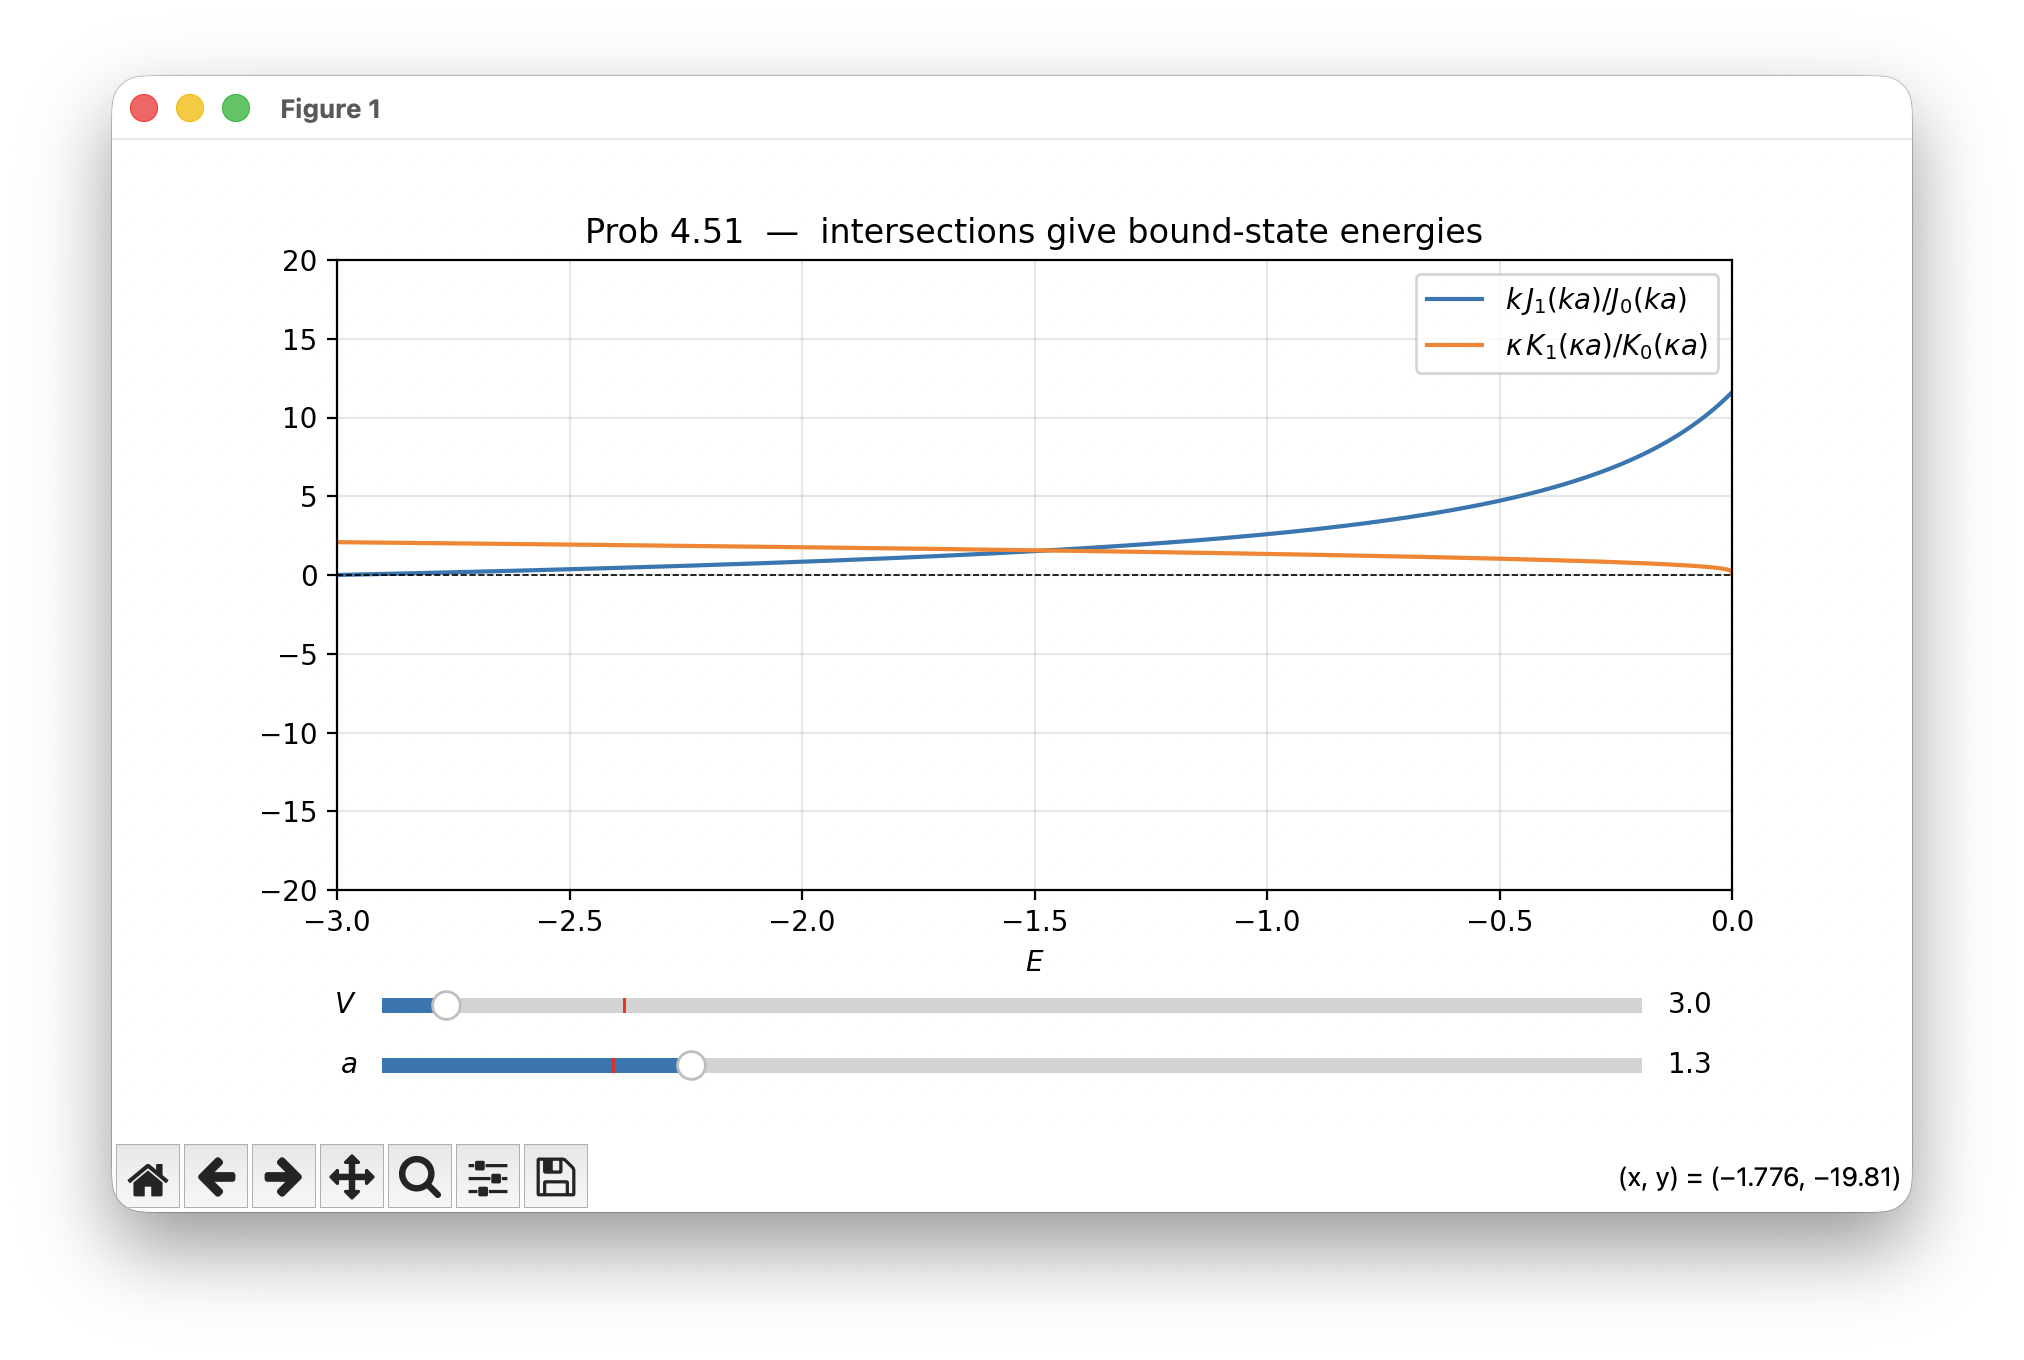
\includegraphics[width=\textwidth]{fig/prob4.51a.png}
        
        \label{fig:sub1}
    \end{subfigure}
    \hfill
    % Second subfigure
    \begin{subfigure}{0.32\textwidth}
        \centering
        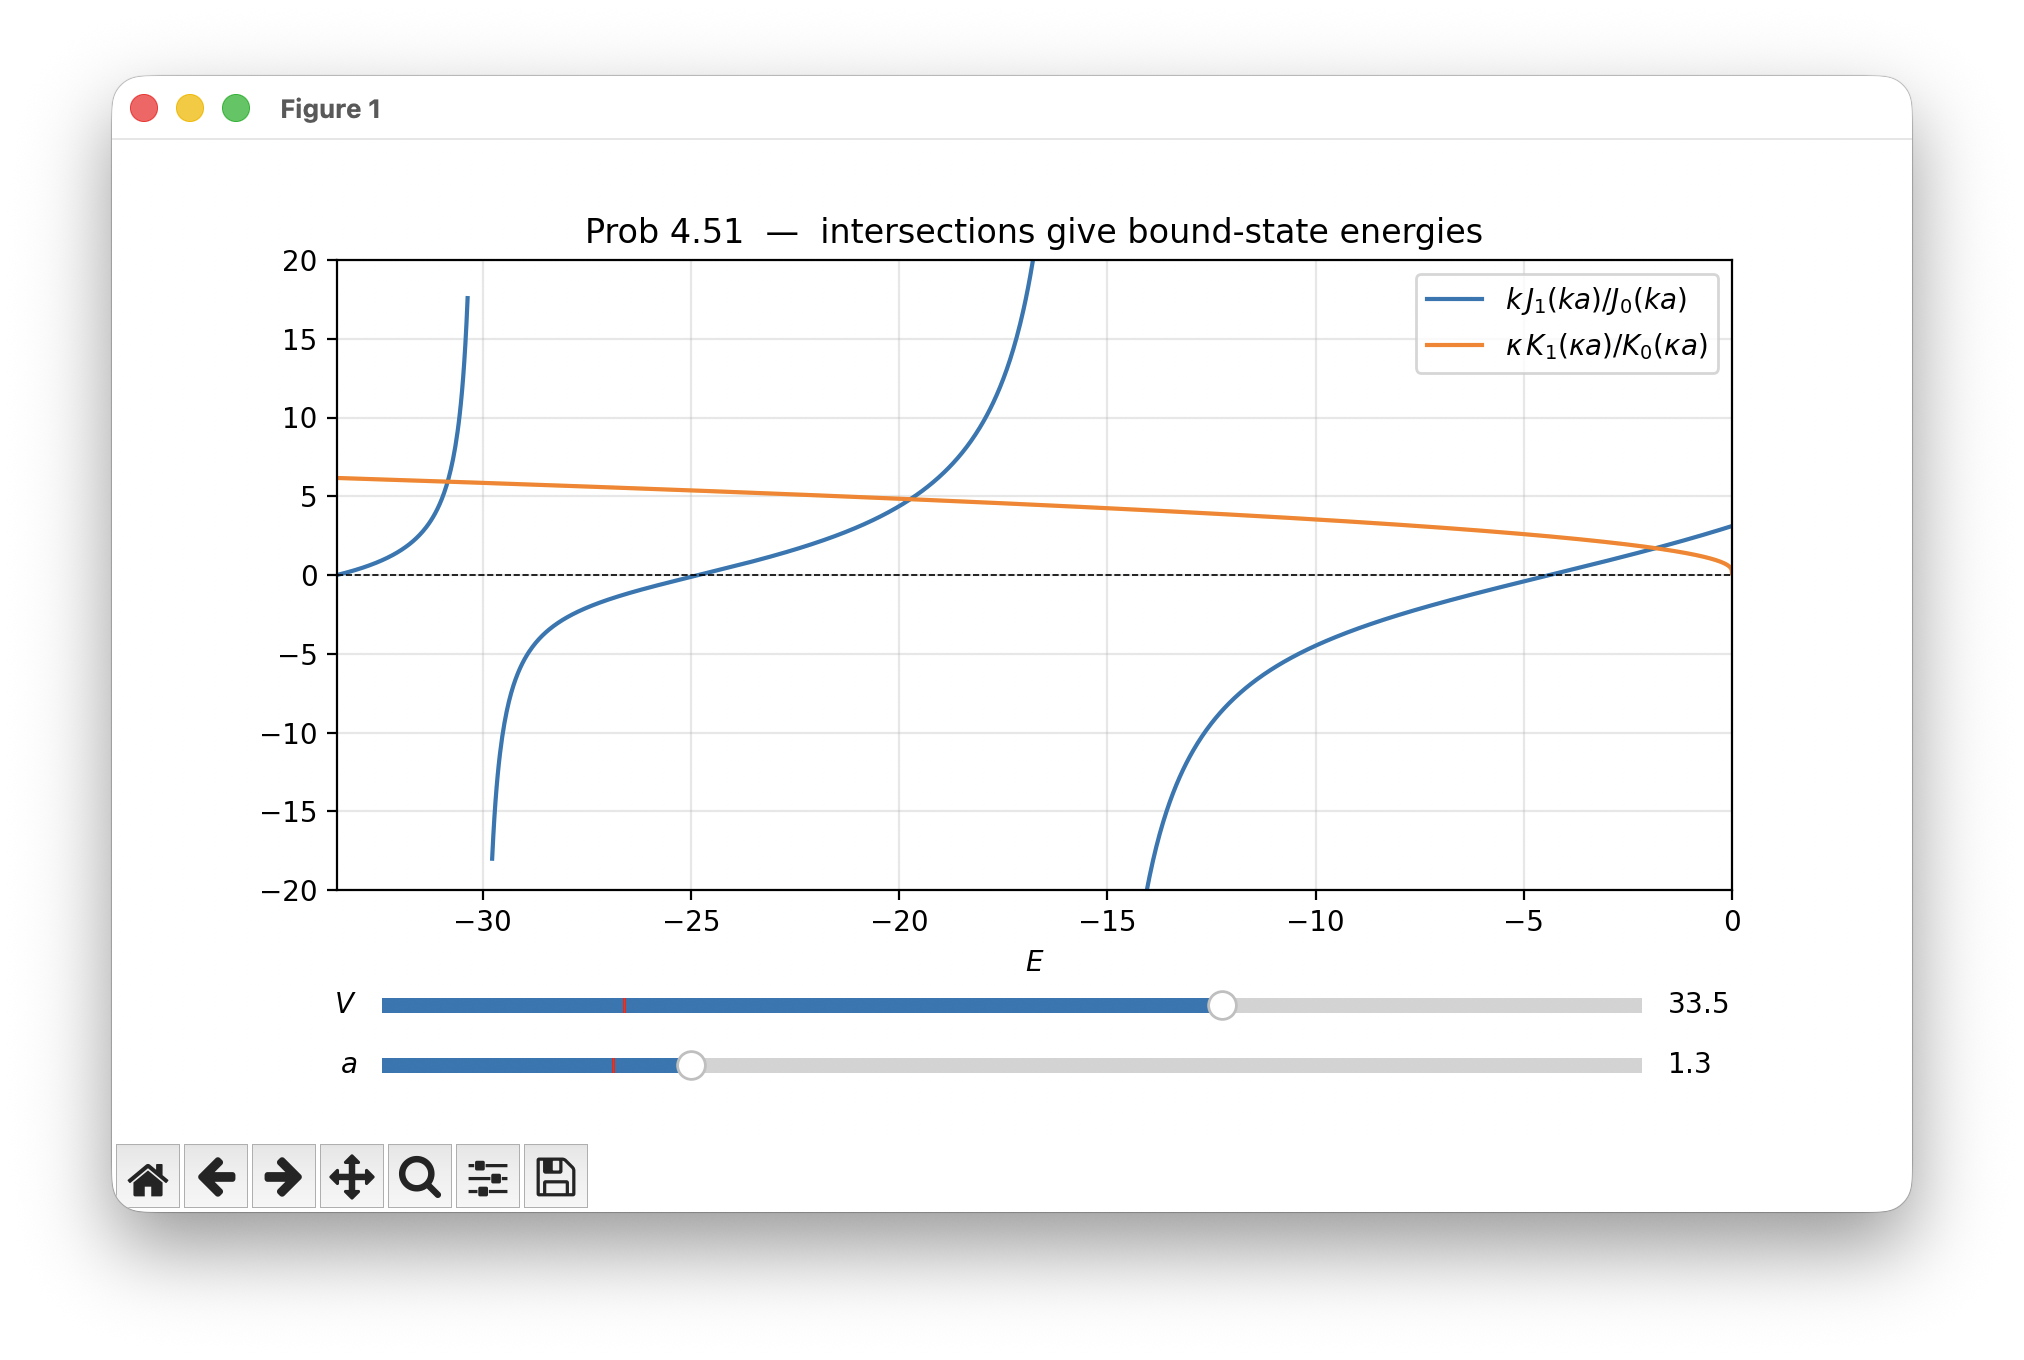
\includegraphics[width=\textwidth]{fig/prob4.51b.png}
        
        \label{fig:sub2}
    \end{subfigure}
    \hfill
    % Third subfigure
    \begin{subfigure}{0.32\textwidth}
        \centering
        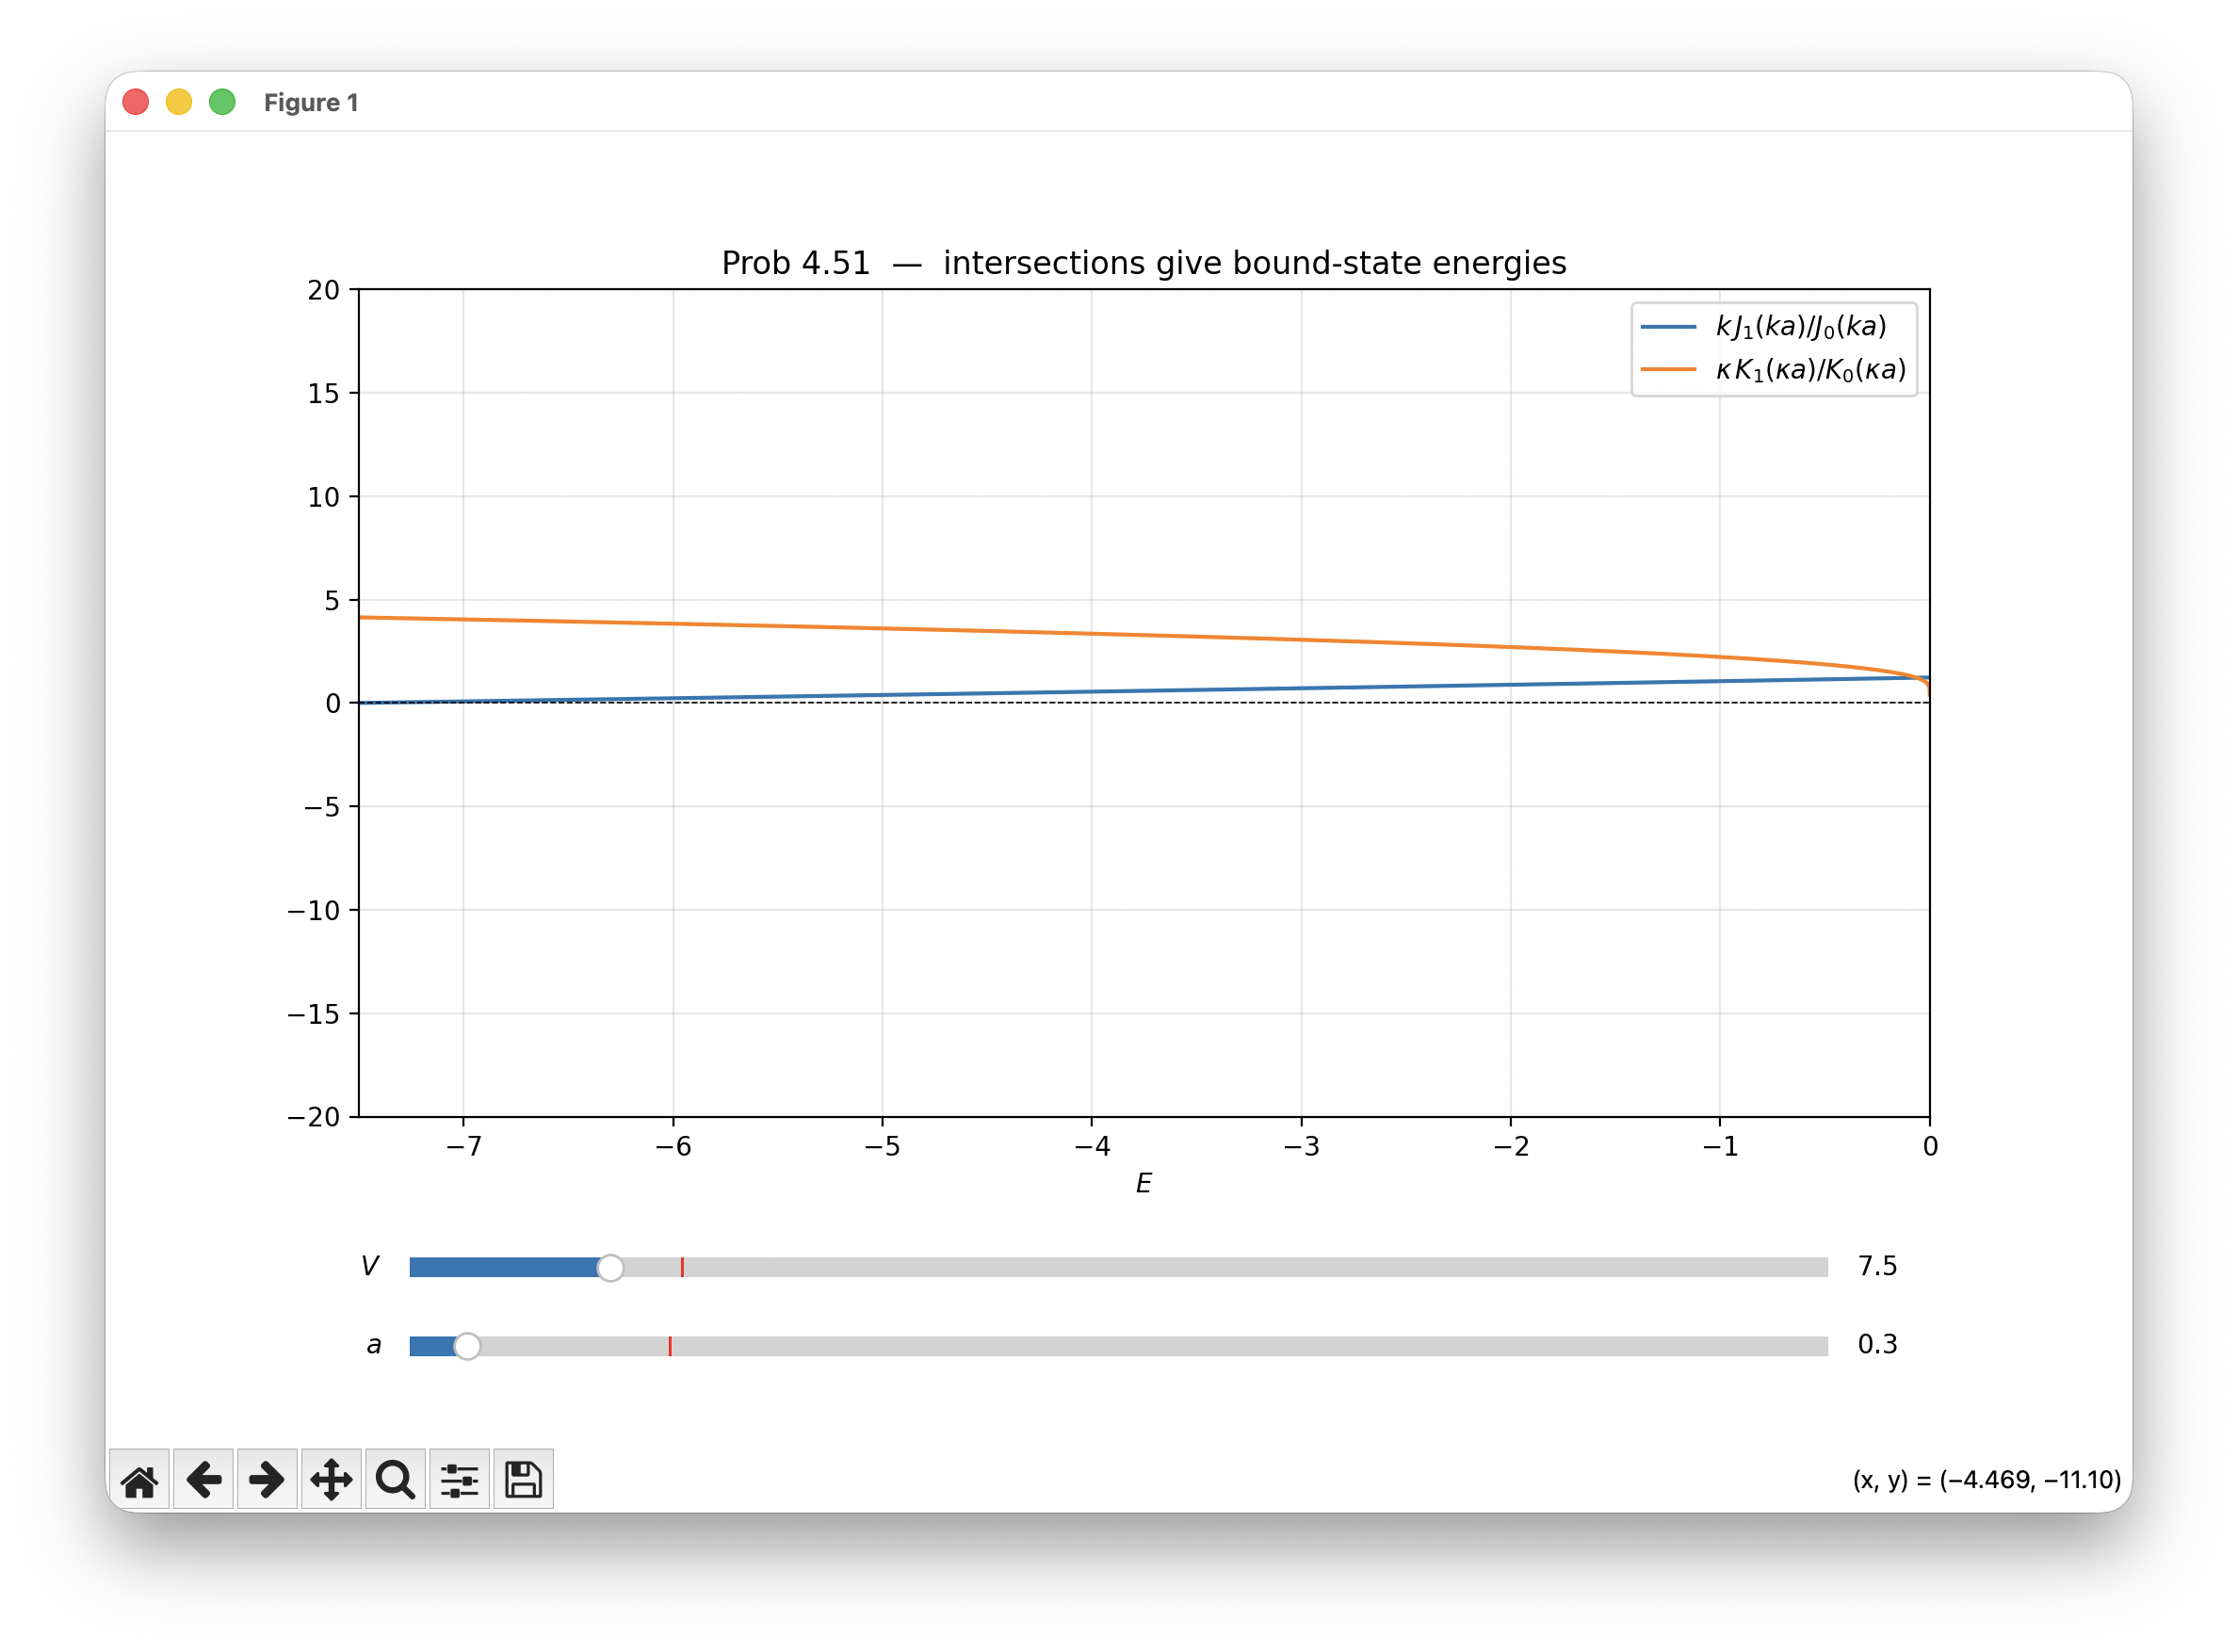
\includegraphics[width=\textwidth]{fig/prob4.51c.png}
        
        \label{fig:sub3}
    \end{subfigure}
    
    \label{fig:2dimwell}
\end{figure}
No matter how shallow or how small the potential well is, there always exists a bound state for $n=0.$
        
        \subsection*{Sol. 52}
        \begin{enumerate}
            \item 
            \begin{align*}
                \psi_{321}(r,\theta,\phi)
            =&
            -\frac{4}{81\sqrt{30}}
            a^{-3/2}
            \left(\frac{r}{a}\right)^2
            \exp(\frac{-r}{3a})
            \left(
            \frac{15}{8\pi}
            \right)^{1/2}
            \sin\theta\cos\theta 
            e^{i\phi}
            \end{align*}
            \item 
            \begin{align*}
                &\int
                \frac{16}{81^2\cdot30}
            a^{-3}
            \left(\frac{r}{a}\right)^4
            \exp(\frac{-2r}{3a})
            \left(
            \frac{15}{8\pi}
            \right)
            \sin^2\theta\cos^2\theta 
            r^2\sin\theta drd\theta d\phi\\
            =&\int 
            \frac{8r^{6} \mathrm{e}^{-\frac{2r}{3a}}}{98415 a^{7}} dr\\
            =&1
            \end{align*}
            \item 
            \begin{align*}
                \langle r^s\rangle=&\int
                \frac{8r^{6+s} \mathrm{e}^{-\frac{2r}{3a}}}{98415 a^{7}}dr\\
                =&
                -
                \frac{1}{720}
                \left(
                \frac{3a}{2}
                \right)^s\Gamma(s+7, \frac{2r}{3a})\bigg|^{\infty}_0\\
                =&\frac{1}{720}
                \left(
                \frac{3a}{2}
                \right)^s
                \Gamma(s+7).
            \end{align*}
            The gamma function is not defined on the non-positive integers, so $s$ is defined for all $\mathbb{R}$ except $s=-7,-8,\dots.$
        \end{enumerate}

        \subsection*{Sol. 53}
        \begin{enumerate}
            \item 
            $$
            \psi_{433}(r,\theta,\phi)
            =-\frac{1}{768\sqrt{35}}
            a^{-3/2}
            \left(\frac{r}{a}\right)^{3}
            \exp\left(\frac{-r}{4a}\right)
            \left(\frac{35}{64\pi}\right)^{1/2}
            \sin^3\theta e^{3i\phi}
            $$
            \item 
            \begin{align*}
                \langle r\rangle
                =&
                \frac{1}{768^2\cdot 35}
            a^{-3}
            \left(\frac{35}{64\pi}\right)
                \int 
                r
            \left(\frac{r}{a}\right)^{6}
            \exp\left(\frac{-r}{2a}\right)
            \sin^6\theta
            r^2\sin\theta  
            drd\theta d\phi \\
            =&
            \frac{1}{768^2\cdot 35}
            a^{-3}
            \left(\frac{35}{64\pi}\right)
            \frac{32}{35}
            2\pi
            \frac{1}{a^6}
                \int 
                r^9            
            \exp\left(\frac{-r}{2a}\right)
            dr\\
            =& 
            18a
            \end{align*}
            \item 
            The eigenvalue of $L^2$ is $\hbar^2l(l+1)=12\hbar^2,$ and the eigenvalue for $L_z$ is $3\hbar.$ The value I could get from $L_x^2+L_y^2$ is $3\hbar^2,$ with probability 1.
        \end{enumerate}
        \subsection*{Sol. 54}
        \begin{enumerate}
            \item $$
            \psi_{100}(r,\theta,\phi)
            =\frac{1}{\sqrt{\pi a^3}}
            e^{-r/a}
            $$
            \begin{align*}
            &\frac{1}{\pi a^3}
                \int_0^b 
                \int_0^\pi 
                \int_0^{2\pi}
                e^{-2r/a}r^2\sin\theta drd\theta 
                d\phi\\
                =&\frac{4}{a^3}
                \int_0^b 
                e^{-2r/a}r^2 dr\\
                =&
                1 - 
                (\frac{2b^2}{a^2} + \frac{2b}{a}+1)\mathrm{e}^{-\frac{2b}{a}}
            \end{align*}
            \item 
            \begin{align*}
                &1 - (\frac{1}{2}\epsilon^2 + \epsilon + 1)
                (1-\epsilon + \frac{1}{2}\epsilon^2-\frac{1}{6}\epsilon^3+\dots)\\
                \approx &
                \frac{1}{6}\epsilon^3\\
                =&\frac{4}{3}\frac{b^3}{a^3}
            \end{align*}
            \item $$
            |\psi(0)|^2
            =\frac{1}{\pi a^3}
            $$
            $$
            \frac{4}{3}\pi b^3
            \frac{1}{\pi a^3} = 
            \frac{4}{3}\frac{b^3}{a^3}
            $$
            \item 
            $$
            1.1\times 10^{-14}.
            $$
        \end{enumerate}
        \subsection*{Sol. 55}
        \begin{enumerate}
            \item 
            $$
            c_{j+1}
            =\frac{2(j+l+1-n)}{(j+1)(j+2l+2)}c_j
            $$
            $$
            c_1 = 
            \frac{2(0)}{(0+1)(0+2n)}c_0 = 0
            $$
            $$
            R_{n(n-1)}(r)
            =\frac{1}{r}\rho^{n}e^{-\rho}c_0
            =N_nr^{n-1}
            e^{-r/(an)}
            $$
            \begin{align*}
                \int_0^\infty 
                N_n^2 r^{2n-2}
                e^{-2r/(an)}r^2dr
                =N_n^2(an)^{2n+1}
                (2n)!\frac{1}{2^{2n+1}}
            \end{align*}
            $$
            N_n = \sqrt{\frac{2^{2n+1}}{(2n)!(an)^{2n+1}}}
            $$
            \item 
            \begin{align*}
                \langle r\rangle
                =& 
                \int rR_{n(n-1)}^2(Y_{(n-1)}^m)^2r^2\sin\theta dr d\theta d\phi\\
                =&
                \frac{2^{2n+1}}{(2n)!(an)^{2n+1}}
                \int r^{2n+1}e^{-2r/(an)}dr\\
                =& 
                \frac{2^{2n+1}}{(2n)!(an)^{2n+1}}
                \frac{(2n+1)!(an)^{2n+2}}{2^{2n+2}}\\
                =&\frac{(an)(2n+1)}{2}
            \end{align*}
            \begin{align*}
                \langle r^2\rangle
                =& 
                \int r^2R_{n(n-1)}^2(Y_{(n-1)}^m)^2r^2\sin\theta dr d\theta d\phi\\
                =&
                \frac{2^{2n+1}}{(2n)!(an)^{2n+1}}
                \int r^{2n+2}e^{-2r/(an)}dr\\
                =& 
                \frac{2^{2n+1}}{(2n)!(an)^{2n+1}}
                \frac{(2n+2)!(an)^{2n+3}}{2^{2n+3}}\\
                =&\frac{(an)^2(2n+1)(2n+2)}{4}
            \end{align*}
            \item 
            \begin{align*}
                \sigma_r = &
            \sqrt{\frac{(an)^2(2n+1)(2n+2)}{4}
            -\frac{(an)^2(2n+1)^2}{4}}\\
            =&\sqrt{\frac{(an)^2(2n+1)}{4}}\\
            =&\frac{\langle r\rangle}{\sqrt{(2n+1)}}
            \end{align*}
        \end{enumerate}

        \subsection*{Sol. 56}
        $$
        \{9, 5\},\;
        \{90, 6\}
        $$
        $$
        \{7, 5\},\;
        \{35, 7\}
        $$
        $$
        \{9, 6\},\;
        \{72, 8\}
        $$

        \subsection*{Sol. 57}
        \begin{enumerate}
            \item By 3.62,
            $$
            \sigma_A^2\sigma_B^2\geq 
            \left(
            \frac{1}{2i}
            \langle[x^2, L_z]\rangle
            \right)^2
            $$
            \begin{align*}
            [x^2, L_z]=&[r^2\sin^2\theta\cos^2\phi, -i\hbar\frac{\partial}{\partial\phi}]\\
            =&-i\hbar r^2\sin^2\theta[\cos^2\phi, \frac{\partial}{\partial\phi}]\\
            =&-i\hbar r^2\sin^2\theta2\sin\phi\cos\phi\\
            =&-2i\hbar xy
        \end{align*}
        Thus
        \begin{align*}
            \sigma_A\sigma_B\geq &
            \hbar
            |\langle
            xy
            \rangle|
        \end{align*}
        \item 
        $L_z$ is a determinate observable in state $\psi_{nlm},$ so $\sigma_B=0.$
        \item In this case, $\langle xy\rangle=0.$
        \end{enumerate}

        \subsection*{Sol. 58}
        \begin{enumerate}
            \item 
            $$
            A = 3
            $$
            \item 
            $
            \frac{1}{2}\hbar 
            $
            with probability $\frac{5}{9},$ and 
            $
            \frac{-1}{2}\hbar 
            $
            with probability $\frac{4}{9}.$
            The expectation value is $\frac{1}{9}\hbar.$
            \item 
            Note that 
            $$
            \frac{1}{3}
            \begin{pmatrix}
                1-2i\\
                2
            \end{pmatrix}
            =
            \frac{3-2i}{3\sqrt{2}}
            \begin{pmatrix}
                \frac{1}{\sqrt{2}}\\
                \frac{1}{\sqrt{2}}
            \end{pmatrix}
            +
            \frac{-1-2i}{3\sqrt{2}}
            \begin{pmatrix}
                \frac{1}{\sqrt{2}}\\
                \frac{-1}{\sqrt{2}}
            \end{pmatrix}
            $$
            $
            \frac{1}{2}\hbar 
            $
            with probability $\frac{13}{18},$ and 
            $
            \frac{-1}{2}\hbar 
            $
            with probability $\frac{5}{18}.$
            The expectation value is $\frac{4}{9}\hbar.$
            \item 
            Note that 
            $$
            \frac{1}{3}
            \begin{pmatrix}
                1-2i\\
                2
            \end{pmatrix}
            =
            \frac{1-4i}{3\sqrt{2}}
            \begin{pmatrix}
                \frac{1}{\sqrt{2}}\\
                \frac{i}{\sqrt{2}}
            \end{pmatrix}
            +
            \frac{i}{3\sqrt{2}}
            \begin{pmatrix}
                \frac{-i}{\sqrt{2}}\\
                \frac{-1}{\sqrt{2}}
            \end{pmatrix}
            $$
            $
            \frac{1}{2}\hbar 
            $
            with probability $\frac{17}{18},$ and 
            $
            \frac{-1}{2}\hbar 
            $
            with probability $\frac{1}{18}.$
            The expectation value is $\frac{8}{9}\hbar.$
        \end{enumerate}

        \subsection*{Sol. 59}
        \begin{align*}
            \langle S_a^{(1)}S_b^{(2)}\rangle= & 
            \frac{1}{2}
            \langle \updownarrows - \downuparrows, 
            S_a^{(1)}S_b^{(2)}
            (\updownarrows - \downuparrows)
            \rangle\\
            =&
            \frac{1}{2}
            \langle S_a^{(1)}\updownarrows, S_b^{(2)}\updownarrows\rangle
            -\frac{1}{2}
            \langle S_a^{(1)}\updownarrows, S_b^{(2)}\downuparrows\rangle
            -\frac{1}{2}
            \langle S_a^{(1)}\downuparrows, S_b^{(2)}\updownarrows\rangle
            +\frac{1}{2}
            \langle S_a^{(1)}\downuparrows, S_b^{(2)}\downuparrows\rangle
        \end{align*}
        By prob4.33
        \begin{align*}
            S_r = \frac{\hbar}{2}
            \begin{pmatrix}
                \cos\theta_r & \sin\theta_r e^{-i\phi_r}\\
                \sin\theta_r e^{i\phi_r} & -\cos\theta_r
            \end{pmatrix}
        \end{align*}
        \begin{align*}
            \langle S_a^{(1)}\updownarrows, S_b^{(2)}\updownarrows\rangle = & 
            \frac{\hbar^2}{4}
            \langle
            \cos\theta_a\updownarrows + 
            \sin\theta_ae^{i\phi_a}\downdownarrows
            ,
            \sin\theta_b e^{-i\phi_b}\upuparrows -
            \cos\theta_b\updownarrows
            \rangle\\
            =&-\frac{\hbar^2}{4}\cos\theta_a\cos\theta_b
        \end{align*}
        \begin{align*}
            \langle S_a^{(1)}\updownarrows, S_b^{(2)}\downuparrows\rangle = & 
            \frac{\hbar^2}{4}
            \langle
            \cos\theta_a\updownarrows + 
            \sin\theta_ae^{i\phi_a}\downdownarrows
            ,
            \cos\theta_b \downuparrows +
            \sin\theta_be^{i\phi_b}\downdownarrows
            \rangle\\
            =&\frac{\hbar^2}{4}\sin\theta_ae^{-i\phi_a}\sin\theta_be^{i\phi_b}
        \end{align*}
        \begin{align*}
            \langle S_a^{(1)}\downuparrows, S_b^{(2)}\updownarrows\rangle = & 
            \frac{\hbar^2}{4}
            \langle
            \sin\theta_ae^{-i\phi_a} \upuparrows -
            \cos\theta_a\downuparrows
            ,
            \sin\theta_b e^{-i\phi_b}\upuparrows -
            \cos\theta_b\updownarrows
            \rangle\\
            =&\frac{\hbar^2}{4}\sin\theta_ae^{i\phi_a}\sin\theta_be^{-i\phi_b}
        \end{align*}
        \begin{align*}
            \langle S_a^{(1)}\downuparrows, S_b^{(2)}\downuparrows\rangle = & 
            \frac{\hbar^2}{4}
            \langle
            \sin\theta_ae^{-i\phi_a} \upuparrows -
            \cos\theta_a\downuparrows
            ,
            \cos\theta_b \downuparrows +
            \sin\theta_be^{i\phi_b}\downdownarrows
            \rangle\\
            =&-\frac{\hbar^2}{4}\cos\theta_a\cos\theta_b
        \end{align*}
        \begin{align*}
            \langle S_a^{(1)}S_b^{(2)}\rangle=&
            -\frac{\hbar^2}{4}\cos\theta_a\cos\theta_b
            -\frac{\hbar^2}{4}\sin\theta_a\sin\theta_b\cos(\phi_a-\phi_b)\\
            =&-\frac{\hbar^2}{4}\bm a_z\bm b_z
            -\frac{\hbar^2}{4}\bm a_x\bm b_x - 
            \frac{\hbar^2}{4}\bm a_y\bm b_y \\
            =&-\frac{\hbar^2}{4}\cos\theta
        \end{align*}
        \subsection*{Sol. 60}
        \begin{enumerate}
        \item 
        
        \begin{align*}
            S_x^{(1)}\bigg|\frac{1}{2}\frac{1}{2}\bigg\rangle
            S_x^{(2)}\bigg|s_2\left(m-\frac{1}{2}\right)\bigg\rangle
            =&\frac{\hbar}{2}\bigg|\frac{1}{2}\frac{-1}{2}\bigg\rangle
            \frac{1}{2}\bigg(
            \hbar\sqrt{s_2(s_2+1)-(m-\frac{1}{2})(m+\frac{1}{2})}
            \bigg|s_2\left(m+\frac{1}{2}\right)\bigg\rangle
            \\&+
            \hbar\sqrt{s_2(s_2+1)-(m-\frac{1}{2})(m-\frac{3}{2})}
            \bigg|s_2\left(m-\frac{3}{2}\right)\bigg\rangle
            \bigg)
        \end{align*}
        \begin{align*}
            S_y^{(1)}\bigg|\frac{1}{2}\frac{1}{2}\bigg\rangle
            S_y^{(2)}\bigg|s_2\left(m-\frac{1}{2}\right)\bigg\rangle
            =&\frac{\hbar}{2}\bigg|\frac{1}{2}\frac{-1}{2}\bigg\rangle
            \frac{1}{2}\bigg(
            \hbar\sqrt{s_2(s_2+1)-(m-\frac{1}{2})(m+\frac{1}{2})}
            \bigg|s_2\left(m+\frac{1}{2}\right)\bigg\rangle
            \\&-
            \hbar\sqrt{s_2(s_2+1)-(m-\frac{1}{2})(m-\frac{3}{2})}
            \bigg|s_2\left(m-\frac{3}{2}\right)\bigg\rangle
            \bigg)
        \end{align*}
        \begin{align*}
            S_z^{(1)}\bigg|\frac{1}{2}\frac{1}{2}\bigg\rangle
            S_z^{(2)}\bigg|s_2\left(m-\frac{1}{2}\right)\bigg\rangle
            =&\frac{\hbar}{2}\bigg|\frac{1}{2}\frac{1}{2}\bigg\rangle
            \hbar\left(m-\frac{1}{2}\right)
            \bigg|s_2\left(m-\frac{1}{2}\right)\bigg\rangle
        \end{align*}
        \begin{align*}
            \bm S^{(1)}\bm S^{(2)}\bigg|\frac{1}{2}\frac{1}{2}\bigg\rangle
            \bigg|s_2\left(m-\frac{1}{2}\right)\bigg\rangle
            =&\\
            \frac{\hbar^2}{2}\sqrt{s_2(s_2+1)-(m-\frac{1}{2})(m+\frac{1}{2})}\bigg|\frac{1}{2}\frac{-1}{2}\bigg\rangle
            \bigg|s_2\left(m+\frac{1}{2}\right)\bigg\rangle
            +
            \frac{\hbar^2}{2}
            \left(m-\frac{1}{2}\right)
            \bigg|\frac{1}{2}\frac{1}{2}\bigg\rangle
            \bigg|s_2\left(m-\frac{1}{2}\right)\bigg\rangle
        \end{align*}
        \begin{align*}
            &S^2\bigg|\frac{1}{2}\frac{1}{2}\bigg\rangle
            \bigg|s_2\left(m-\frac{1}{2}\right)\bigg\rangle
            =\hbar^2\frac{3}{4}\bigg|\frac{1}{2}\frac{1}{2}\bigg\rangle
            \bigg|s_2\left(m-\frac{1}{2}\right)\bigg\rangle
            +
            \hbar^2s_2(s_2+1)\bigg|\frac{1}{2}\frac{1}{2}\bigg\rangle
            \bigg|s_2\left(m-\frac{1}{2}\right)\bigg\rangle\\
            &+\hbar^2\sqrt{s_2(s_2+1)-(m-\frac{1}{2})(m+\frac{1}{2})}\bigg|\frac{1}{2}\frac{-1}{2}\bigg\rangle
            \bigg|s_2\left(m+\frac{1}{2}\right)\bigg\rangle
            +
            \hbar^2
            \left(m-\frac{1}{2}\right)
            \bigg|\frac{1}{2}\frac{1}{2}\bigg\rangle
            \bigg|s_2\left(m-\frac{1}{2}\right)\bigg\rangle\\
            =&\hbar^2\sqrt{s_2(s_2+1)-(m-\frac{1}{2})(m+\frac{1}{2})}\bigg|\frac{1}{2}\frac{-1}{2}\bigg\rangle
            \bigg|s_2\left(m+\frac{1}{2}\right)\bigg\rangle\\
            &+
            \hbar^2(s_2(s_2+1)+m+\frac{1}{4})
            \bigg|\frac{1}{2}\frac{1}{2}\bigg\rangle
            \bigg|s_2\left(m-\frac{1}{2}\right)\bigg\rangle
        \end{align*}
        
        \begin{align*}
            S_x^{(1)}\bigg|\frac{1}{2}\frac{-1}{2}\bigg\rangle
            S_x^{(2)}\bigg|s_2\left(m+\frac{1}{2}\right)\bigg\rangle
            =&\frac{\hbar}{2}\bigg|\frac{1}{2}\frac{1}{2}\bigg\rangle
            \frac{1}{2}\bigg(
            \hbar\sqrt{s_2(s_2+1)-(m+\frac{1}{2})(m+\frac{3}{2})}
            \bigg|s_2\left(m+\frac{3}{2}\right)\bigg\rangle
            \\&+
            \hbar\sqrt{s_2(s_2+1)-(m+\frac{1}{2})(m-\frac{1}{2})}
            \bigg|s_2\left(m-\frac{1}{2}\right)\bigg\rangle
            \bigg)
        \end{align*}
        \begin{align*}
            S_y^{(1)}\bigg|\frac{1}{2}\frac{-1}{2}\bigg\rangle
            S_y^{(2)}\bigg|s_2\left(m+\frac{1}{2}\right)\bigg\rangle
            =&-\frac{\hbar}{2}\bigg|\frac{1}{2}\frac{1}{2}\bigg\rangle
            \frac{1}{2}\bigg(
            \hbar\sqrt{s_2(s_2+1)-(m+\frac{1}{2})(m+\frac{3}{2})}
            \bigg|s_2\left(m+\frac{3}{2}\right)\bigg\rangle
            \\&-
            \hbar\sqrt{s_2(s_2+1)-(m+\frac{1}{2})(m-\frac{1}{2})}
            \bigg|s_2\left(m-\frac{1}{2}\right)\bigg\rangle
            \bigg)
        \end{align*}
        \begin{align*}
            S_z^{(1)}\bigg|\frac{1}{2}\frac{-1}{2}\bigg\rangle
            S_z^{(2)}\bigg|s_2\left(m+\frac{1}{2}\right)\bigg\rangle
            =&\frac{-\hbar}{2}\bigg|\frac{1}{2}\frac{-1}{2}\bigg\rangle
            \hbar\left(m+\frac{1}{2}\right)
            \bigg|s_2\left(m+\frac{1}{2}\right)\bigg\rangle
        \end{align*}

        \begin{align*}
            \bm S^{(1)}\bm S^{(2)}\bigg|\frac{1}{2}\frac{-1}{2}\bigg\rangle
            \bigg|s_2\left(m+\frac{1}{2}\right)\bigg\rangle
            =&\\
            \frac{\hbar^2}{2}\sqrt{s_2(s_2+1)-(m+\frac{1}{2})(m-\frac{1}{2})}\bigg|\frac{1}{2}\frac{1}{2}\bigg\rangle
            \bigg|s_2\left(m-\frac{1}{2}\right)\bigg\rangle
            -
            \frac{\hbar^2}{2}
            \left(m+\frac{1}{2}\right)
            \bigg|\frac{1}{2}\frac{-1}{2}\bigg\rangle
            \bigg|s_2\left(m+\frac{1}{2}\right)\bigg\rangle
        \end{align*}
        \begin{align*}
            &S^2\bigg|\frac{1}{2}\frac{-1}{2}\bigg\rangle
            \bigg|s_2\left(m+\frac{1}{2}\right)\bigg\rangle
            =\hbar^2\frac{3}{4}\bigg|\frac{1}{2}\frac{-1}{2}\bigg\rangle
            \bigg|s_2\left(m+\frac{1}{2}\right)\bigg\rangle
            +
            \hbar^2s_2(s_2+1)\bigg|\frac{1}{2}\frac{-1}{2}\bigg\rangle
            \bigg|s_2\left(m+\frac{1}{2}\right)\bigg\rangle\\
            &+\hbar^2\sqrt{s_2(s_2+1)-(m-\frac{1}{2})(m+\frac{1}{2})}\bigg|\frac{1}{2}\frac{1}{2}\bigg\rangle
            \bigg|s_2\left(m-\frac{1}{2}\right)\bigg\rangle
            -
            \hbar^2
            \left(m+\frac{1}{2}\right)
            \bigg|\frac{1}{2}\frac{-1}{2}\bigg\rangle
            \bigg|s_2\left(m+\frac{1}{2}\right)\bigg\rangle\\
            =&\hbar^2\sqrt{s_2(s_2+1)-(m-\frac{1}{2})(m+\frac{1}{2})}\bigg|\frac{1}{2}\frac{1}{2}\bigg\rangle
            \bigg|s_2\left(m-\frac{1}{2}\right)\bigg\rangle\\
            &+
            \hbar^2(s_2(s_2+1)-m+\frac{1}{4})
            \bigg|\frac{1}{2}\frac{-1}{2}\bigg\rangle
            \bigg|s_2\left(m+\frac{1}{2}\right)\bigg\rangle
        \end{align*}
        
        \begin{align*}
            s(s+1)A = (s_2(s_2+1)+m+\frac{1}{4})A + \sqrt{s_2(s_2+1)-(m-\frac{1}{2})(m+\frac{1}{2})}B
        \end{align*}
        \begin{align*}
            s(s+1)B = \sqrt{s_2(s_2+1)-(m-\frac{1}{2})(m+\frac{1}{2})}A + (s_2(s_2+1)-m+\frac{1}{4})B
        \end{align*}
        Let $a=s_2(s_2+1)+\frac{1}{4},$ $b=\sqrt{s_2(s_2+1)-(m-\frac{1}{2})(m+\frac{1}{2})},$ then
        $$
        \frac{A}{B} = \frac{(a+m)A + bB}{bA + (a-m)B}
        $$
        $$
        b(\frac{A}{B})^2 + (-2m)\frac{A}{B} - b= 0
        $$
        $$
        \frac{A}{B} = \frac{2m\pm\sqrt{4m^2+4b^2}}{2b}
    =   \frac{m\pm\sqrt{s_2(s_2+1)+\frac{1}{4}}}{\sqrt{s_2(s_2+1)-m^2+\frac{1}{4}}} = \frac{m\pm(s_2+\frac{1}{2})}{\sqrt{(s_2+\frac{1}{2})^2-m^2}}
        $$
If plus, then 
$$
\frac{A}{B} = \sqrt{\frac{s_2+\frac{1}{2}+m}{s_2+\frac{1}{2}-m}},
$$
if minus, then 
$$
\frac{A}{B} = -\sqrt{\frac{s_2+\frac{1}{2}-m}{s_2+\frac{1}{2}+m}}.
$$
Combine with the fact that $A^2+B^2=1,$ we have 
$$
B = \pm\sqrt{\frac{s_2+\frac{1}{2}\mp m}{2s_2+1}}, 
A = \sqrt{\frac{s_2+\frac{1}{2}\pm m}{2s_2+1}}.
$$
\item 
    $$
    |10\rangle =
    \sqrt{\frac{\frac{1}{2}+\frac{1}{2}}{2\cdot 
    \frac{1}{2} + 1}}
    |\frac{1}{2}\frac{1}{2}
    \frac{1}{2}\frac{-1}{2}\rangle
    +
    \sqrt{\frac{\frac{1}{2}+\frac{1}{2}}{2\cdot 
    \frac{1}{2} + 1}}
    |\frac{1}{2}\frac{1}{2}
    \frac{-1}{2}\frac{1}{2}\rangle
    =
    \sqrt{\frac{1}{2}}
   |\frac{1}{2}\frac{1}{2}
    \frac{1}{2}\frac{-1}{2}\rangle
    +
    \sqrt{\frac{1}{2}}
    |\frac{1}{2}\frac{1}{2}
    \frac{-1}{2}\frac{1}{2}\rangle
    $$
    $$
    |\frac{3}{2}\frac{-1}{2}\rangle =
    \sqrt{\frac{1+\frac{1}{2}+\frac{1}{2}}{2\cdot 
    1 + 1}}
    |1\frac{1}{2}
    0\frac{-1}{2}\rangle
    +
    \sqrt{\frac{1+\frac{1}{2}-\frac{1}{2}}{2\cdot 
    1 + 1}}
    |1\frac{1}{2}
    (-1)\frac{1}{2}\rangle
    =
    \sqrt{\frac{2}{3}}
    |1\frac{1}{2}
    0\frac{-1}{2}\rangle
    +
    \sqrt{\frac{1}{3}}
    |1\frac{1}{2}
    (-1)\frac{1}{2}\rangle
    $$
    $$
    |\frac{3}{2}\frac{1}{2}\rangle =
    -\sqrt{\frac{2+\frac{1}{2}+\frac{1}{2}}{2\cdot 
    2 + 1}}
    |2\frac{1}{2}
    1\frac{-1}{2}\rangle
    +
    \sqrt{\frac{2+\frac{1}{2}-\frac{1}{2}}
    {2\cdot 2 + 1}}
    |2\frac{1}{2}
    0\frac{1}{2}\rangle
    =
    -\sqrt{\frac{3}{5}}
    |2\frac{1}{2}
    1\frac{-1}{2}\rangle
    +
    \sqrt{\frac{2}{5}}
    |2\frac{1}{2}
    0\frac{1}{2}\rangle
    $$
\end{enumerate}
\subsection*{Sol. 61}
$$
S_+ \chi_{-3/2}
=\hbar\sqrt{(\frac{3}{2}\frac{5}{2} - (-\frac{3}{2})(-\frac{1}{2}))} \chi_{-1/2}
=\hbar\sqrt{3}\chi_{-1/2}
$$
$$
S_+ \chi_{-1/2}
=\hbar\sqrt{(\frac{3}{2}\frac{5}{2} - (-\frac{1}{2})(\frac{1}{2}))} \chi_{1/2}
=\hbar2\chi_{1/2}
$$
$$
S_+ \chi_{1/2}
=\hbar\sqrt{(\frac{3}{2}\frac{5}{2} - (\frac{1}{2})(\frac{3}{2}))} \chi_{3/2}
=\hbar\sqrt{3}\chi_{3/2}
$$
$$
S_- \chi_{3/2}
=\hbar\sqrt{(\frac{3}{2}\frac{5}{2} - (\frac{3}{2})(\frac{1}{2}))} \chi_{1/2}
=\hbar\sqrt{3}\chi_{1/2}
$$
$$
S_- \chi_{1/2}
=\hbar\sqrt{(\frac{3}{2}\frac{5}{2} - (\frac{1}{2})(-\frac{1}{2}))} \chi_{-1/2}
=\hbar2\chi_{-1/2}
$$
$$
S_- \chi_{-1/2}
=\hbar\sqrt{(\frac{3}{2}\frac{5}{2} - (-\frac{1}{2})(-\frac{3}{2}))} \chi_{-3/2}
=\hbar\sqrt{3}\chi_{-3/2}
$$
\begin{align*}
    &S_+ = \hbar\begin{pmatrix}
        0 & \sqrt{3} & 0  & 0\\
        0 & 0 & 2  & 0\\
        0 & 0 & 0  & \sqrt{3}\\
        0 & 0 & 0  & 0\\
    \end{pmatrix}\\
    &S_- = \hbar\begin{pmatrix}
        0 & 0 & 0  & 0\\
        \sqrt{3} & 0 & 0  & 0\\
        0 & 2 & 0  & 0\\
        0 & 0 & \sqrt{3}  & 0\\
    \end{pmatrix}\\
    &S_x = \frac{\hbar}{2}
    \begin{pmatrix}
        0 & \sqrt{3} & 0  & 0\\
        \sqrt{3} & 0 & 2  & 0\\
        0 & 2 & 0  & \sqrt{3}\\
        0 & 0 & \sqrt{3}  & 0\\
    \end{pmatrix}
\end{align*}
Characteristic equation:
\begin{align*}
    ch_T(t) = (t-\frac{\hbar}{2})
    (t+\frac{\hbar}{2})
    (t-\frac{3\hbar}{2})
    (t+\frac{3\hbar}{2})
\end{align*}
\subsection*{Sol. 62}
Let $v_s, v_{s-1},\dots, v_{-s}$ be a basis of a spin $s$ system. Then 
$$
S_zv_j = \hbar j v_j.
$$
$$
S_+v_j 
= \hbar \sqrt{s(s+1)-j(j+1)}v_{j+1}
=\hbar \sqrt{(s+j+1)(s-j)}v_{j+1}
=\hbar b_{j+1}v_{j+1}.
$$
$$
S_-v_j = \hbar \sqrt{s(s+1)-j(j-1)}v_{j-1}
=\hbar \sqrt{(s+j)(s-j+1)}v_{j-1}=\hbar b_jv_j.
$$

\begin{align*}
    S_xv_j = \frac{\hbar}{2}(b_{j+1}v_{j+1} + b_j v_j)
\end{align*}
\begin{align*}
    S_yv_j = \frac{\hbar}{2i}(b_{j+1}v_{j+1} - b_j v_j)
\end{align*}

\subsection*{Sol. 63}
\begin{align*}
    L_+Y^m_l=&\hbar\sqrt{(l-m)(l+m+1)}
    K^{m+1}_le^{i(m+1)\phi}P^{m+1}_l(\cos\theta)\\
    =&\hbar e^{i\phi}(\frac{\partial}{\partial\theta}+i\cot\theta\frac{\partial}{\partial\phi})
    K^m_le^{im\phi}P^m_l(\cos\theta)\\
    =&\hbar e^{i\phi}K^m_l
    (e^{im\phi}P^{m'}_l(\cos\theta)(-\sin\theta)
    +i\cot\theta P^{m}_l(\cos\theta)(im)e^{im\phi})\\
    =&\hbar e^{i(m+1)\phi}K^m_l
    (-\sin\theta (-\frac{\sqrt{1-\cos^2\theta}}{1-\cos^2\theta}P^{m+1}_l(\cos\theta) - 
    m\frac{\cos\theta}{1-\cos^2\theta}P^m_l(\cos\theta))
    -m\cot\theta P^{m}_l(\cos\theta))\\
    =&\hbar e^{i(m+1)\phi}K_l^mP^{m+1}_l(\cos\theta).
\end{align*}
We obtain the relation
$$
\sqrt{(l-m)(l+m+1)}K_l^{m+1} = K^m_l,
$$
and thus we have $ \sqrt{\frac{(l+m)!}{(l-m)!}}K^m_l =K^0_l.$
By problem 4.25,
\begin{align*}
    K^{l}_lP^l_l(\cos\theta)
    =
    \frac{1}{\sqrt{(2l)!}}K^0_l
    (-1)^l\sin^l\theta \frac{(2l)!}{2^l l!}=(-1)^l\sqrt{\frac{(2l+1)!}{\pi}}\frac{1}{2^{l+1}l!}\sin^l\theta.
\end{align*}
\begin{align*}
    K^0_l = 
    \sqrt{\frac{(2l+1)}{\pi}}\frac{1}{2}
\end{align*}
\begin{align*}
    K^m_l 
    =\sqrt{\frac{(2l+1)}{4\pi}
    \frac{(l-m)!}{(l+m)!}}.
\end{align*}

\subsection*{Sol. 64}
\begin{enumerate}
    \item $2\hbar^2$ with probability 1.
    \item $0$ with probability $\frac{1}{3}$, 
    $\hbar$ with probability $\frac{2}{3}$.
    \item $\frac{3}{4}\hbar^2$ with probability 1.
    \item $\frac{1}{2}\hbar$ with probability $\frac{1}{3}$, 
    $\frac{-1}{2}\hbar$  with probability $\frac{2}{3}$.
    \item 
    $$
    |10\rangle|\frac{1}{2}\frac{1}{2}\rangle = 
    \sqrt{\frac{2}{3}}|\frac{3}{2}\frac{1}{2}\rangle -
    \sqrt{\frac{1}{3}}|\frac{1}{2}\frac{1}{2}\rangle
    $$
    $$
    |11\rangle|\frac{1}{2}\frac{-1}{2}\rangle = 
    \sqrt{\frac{1}{3}}|\frac{3}{2}\frac{1}{2}\rangle +
    \sqrt{\frac{2}{3}}|\frac{1}{2}\frac{1}{2}\rangle
    $$
    The state becomes 
    $$
    \frac{2\sqrt{2}}{3}|\frac{3}{2}\frac{1}{2}\rangle +
    \frac{1}{3}|\frac{1}{2}\frac{1}{2}\rangle
    $$
    $\frac{15}{4}\hbar^2$ with probability $\frac{8}{9}$, 
    $\frac{3}{4}\hbar^2$  with probability $\frac{1}{9}$.
    \item $\frac{1}{2}\hbar$ with probability $1.$
    \item 
    The position probability density is 
    \begin{align*}
        &R_{21}^2\left|\sqrt{\frac{1}{3}}Y^0_1 + \sqrt{\frac{2}{3}}Y^1_1\right|^2r^2\sin\theta\\
        =&
        \frac{1}{24}a^{-3}\frac{r^2}{a^2}\exp(\frac{-r}{a})
        \left|\sqrt{\frac{1}{3}}\sqrt{\frac{3}{4\pi}}\cos\theta -\sqrt{\frac{2}{3}}\sqrt{\frac{3}{8\pi}}
        \sin\theta e^{i\phi}\right|^2
        r^2\sin\theta\\
        =&\frac{1}{96\pi}\frac{r^4}{a^5}
        \exp\left(\frac{-r}{a}\right)\sin\theta
        (1-2\sin2\theta\cos\phi).
        \end{align*}
        \item 
        The probability density of finding the particle with spin up at radius $r$ is 
        $$
        \frac{1}{3}\frac{1}{24}\frac{r^4}{a^5}
        \exp\left(\frac{-r}{a}\right).
        $$
\end{enumerate}

\subsection*{Sol. 65}
$$
|\frac{3}{2}\frac{3}{2}\rangle = 
|\uparrow\uparrow\uparrow\rangle
$$
\begin{align*}
    S_-|\uparrow\uparrow\uparrow\rangle
=&(S_-^{(1)}|\uparrow\rangle)|\uparrow\uparrow\rangle
+|\uparrow\rangle(S_-^{(2)}|\uparrow\rangle)|\uparrow\rangle
+
|\uparrow\uparrow\rangle(S_-^{(3)}|\uparrow\rangle)\\
=&\hbar
(|\downarrow\uparrow\uparrow\rangle + 
|\uparrow\downarrow\uparrow\rangle
+|\uparrow\uparrow\downarrow\rangle
),
\end{align*}
so 
$$
|\frac{3}{2}\frac{1}{2}\rangle = 
\frac{1}{\sqrt{3}}|\downarrow\uparrow\uparrow\rangle + 
\frac{1}{\sqrt{3}}|\uparrow\downarrow\uparrow\rangle+
\frac{1}{\sqrt{3}}|\uparrow\uparrow\downarrow\rangle
$$
\begin{align*}
    &(S_-^{(1)} + S_-^{(2)} + S_-^{(3)})
 (|\downarrow\uparrow\uparrow\rangle + 
|\uparrow\downarrow\uparrow\rangle
+|\uparrow\uparrow\downarrow\rangle
)
\propto
(|\downarrow\downarrow\uparrow\rangle + |\downarrow\uparrow\downarrow\rangle +
|\uparrow\downarrow\downarrow\rangle),
\end{align*}
so 
$$
|\frac{3}{2}\frac{-1}{2}\rangle = 
\frac{1}{\sqrt{3}}|\downarrow\downarrow\uparrow\rangle + 
\frac{1}{\sqrt{3}}|\downarrow\uparrow\downarrow\rangle+
\frac{1}{\sqrt{3}}|\uparrow\downarrow\downarrow\rangle,
$$
and 
$$
|\frac{3}{2}\frac{-3}{2}\rangle = 
|\downarrow\downarrow\downarrow\rangle.
$$
$$
|\frac{1}{2}\frac{1}{2}\rangle_1
=\frac{1}{\sqrt{2}}
(|\uparrow\downarrow\uparrow\rangle-|\downarrow\uparrow\uparrow\rangle)
$$
$$
|\frac{1}{2}\frac{-1}{2}\rangle_1
=
\frac{1}{\sqrt{2}}
(|\uparrow\downarrow\downarrow\rangle-|\downarrow\uparrow\downarrow\rangle)
$$
$$
|\frac{1}{2}\frac{1}{2}\rangle_2
=\frac{1}{\sqrt{2}}
(|\uparrow\uparrow\downarrow\rangle - |\downarrow\uparrow\uparrow\rangle)
$$
$$
|\frac{1}{2}\frac{-1}{2}\rangle_2   
=
\frac{1}{\sqrt{2}}
(|\uparrow\downarrow\downarrow\rangle - |\downarrow\downarrow\uparrow\rangle).
$$

\subsection*{Sol. 66}
By prob4.31 and by Ch3.5.1, to attain the minimum uncertainty bound, we must satisfy
\begin{align*}
    (S_y-\langle S_y\rangle)\begin{pmatrix}
        a \\ b
    \end{pmatrix}
    =ir
    (S_x-\langle S_x\rangle)\begin{pmatrix}
        a \\ b
    \end{pmatrix}
\end{align*}
for some real number $r.$
\begin{align*}
    \frac{\hbar}{2}i\begin{pmatrix}
        -b \\ a
    \end{pmatrix}
    -\frac{\hbar}{2}(-i\bar ab+i\bar ba)\begin{pmatrix}
        a\\b
    \end{pmatrix}
    =\frac{\hbar}{2}ir\begin{pmatrix}
        b\\a
    \end{pmatrix}
    -ir\frac{\hbar}{2}
    (\bar ab+\bar ba)
    \begin{pmatrix}
        a\\b
    \end{pmatrix}
\end{align*}
\begin{align*}
    -b-(-\bar ab + \bar ba)a = rb - r(\bar a b + \bar b a)a
\end{align*}
\begin{align*}
    a-(-\bar ab + \bar ba)b = ra - r(\bar a b + \bar b a)b
\end{align*}
\begin{align*}
    r = \frac{-b -(-\bar ab+\bar ba )a}{b-(\bar ab +\bar ba)a}
    =\frac{a-(-\bar a b + \bar ba)b}{a-(\bar a b + \bar ba)b}
\end{align*}
Note that 
\begin{align*}
    -ab + (\bar ab+\bar ba)b^2 - (-\bar ab+\bar ba)a^2 = ab
    -(-\bar ab+\bar ba)b^2 - (\bar ab + \bar ba)a^2
\end{align*}
\begin{align*}
    -ab + a\bar bb^2 +\bar a ba^2 = 0
\end{align*}
\begin{align*}
    ab(-1 + |b|^2 + |a|^2) = 0,
\end{align*}
these two are guaranteed to be equal.
To ensure $r$ to be real
\begin{align*}
    \frac{a-(-\bar a b + \bar ba)b}{a-(\bar a b + \bar ba)b} = 
    \frac{\bar a-(-a \bar b + b\bar a)\bar b}
    {\bar a-( a \bar b + b\bar a)\bar b}
\end{align*}
\begin{align*}
    &a\bar a - a(a\bar b + b\bar a)\bar b
    -\bar a(-\bar a b + \bar ba)b 
    +(-\bar ab + \bar ba)(a\bar b + b\bar a)b\bar b\\
    =&a\bar a - a(-a\bar b + b\bar a)\bar b -
    \bar a(\bar ab+\bar ba)b + (\bar a b+\bar ba)(-a\bar b+b\bar a)b\bar b
\end{align*}
\begin{align*}
    -a^2\bar b^2 + \bar a^2b^2 - \bar a^2b^2 b\bar b + \bar b^2a^2b\bar b = 0
\end{align*}
\begin{align*}
    (1-b\bar b)(\bar a^2 b^2 - a^2\bar b^2) = 0
\end{align*}
The condition holds when $\bar a
^2b^2$ is real.

\subsection*{Sol. 67}
\begin{enumerate}
    \item 
    \begin{align*}
        S^2 =& (\bm S_1+\bm S_2 + \bm S_3)^2\\
        =&S_1^2 + S_2^2 + S_3^2 +
        2\bm S_1\cdot \bm S_2
        +2\bm S_2\cdot \bm S_3
        +2\bm S_1\cdot \bm S_3\\
        =&\frac{9}{4}\hbar^2 + 2\frac{H}{J}
    \end{align*}
    $$
    H = \frac{J}{2}(S^2-\frac{9}{4}\hbar^2)
    $$
    \item 
    The lowest possible total spin is 
    $\frac{3}{4}\hbar^2,$ so the ground sate energy is 
    $-\frac{3}{4}\hbar^2J.$
    By problem4.65, the degeneracy is 4.
    \item 
    \begin{align*}
        &S^2 - (\bm S_1 + \bm S_3)^2 - (\bm S_2 + \bm S_4)^2\\
        =&
        S_1^2+ S_2^2 + S_3^2 + S_4^2 +
        2\bm S_1\cdot \bm S_2
        +2\bm S_1\cdot \bm S_3
        +2\bm S_1\cdot \bm S_4
        +2\bm S_2\cdot \bm S_3\\
        &+2\bm S_2\cdot \bm S_4
        +2\bm S_3\cdot \bm S_4
        -S_1^2-S_3^2-2\bm S_1\cdot \bm S_3
        -S_2^2 - S_4^2 - 2\bm S_2\cdot \bm S_4
        \\
        =&
         2\bm S_1\cdot \bm S_2
        +2\bm S_1\cdot \bm S_4
        +2\bm S_2\cdot \bm S_3
        +2\bm S_3\cdot \bm S_4
    \end{align*}
    so
    $$
    H = \frac{1}{2}J\left[S^2 - (\bm S_1+\bm S_3)^2 - (\bm S_2 + \bm S_4)^2\right]
    $$
    The ground state energy is to let the total spin 0, and the two subsystems be of spin 1, and therefore
    $-2\hbar^2J$
 \end{enumerate}
 \subsection*{Sol. 68}
 \begin{enumerate}
     \item 
     \begin{align*}
         v_j =& (-\frac{e^2}{4\pi\epsilon_0}\frac{1}{bj/(N+1)}
         +\frac{\hbar^2}{2m_e}\frac{l(l+1)}{(bj/(N+1))^2})\frac{2m_e(b/(N+1))^2}{\hbar^2}\\
         =&
          -\frac{e^22m_e}{4\pi\epsilon_0\hbar^2}
          \frac{b}{j(N+1)}
          +\frac{l(l+1)}{j^2}\\
          =&-\frac{2b}{ja(N+1)} + \frac{l(l+1)}{j^2}
     \end{align*}
     \item 
     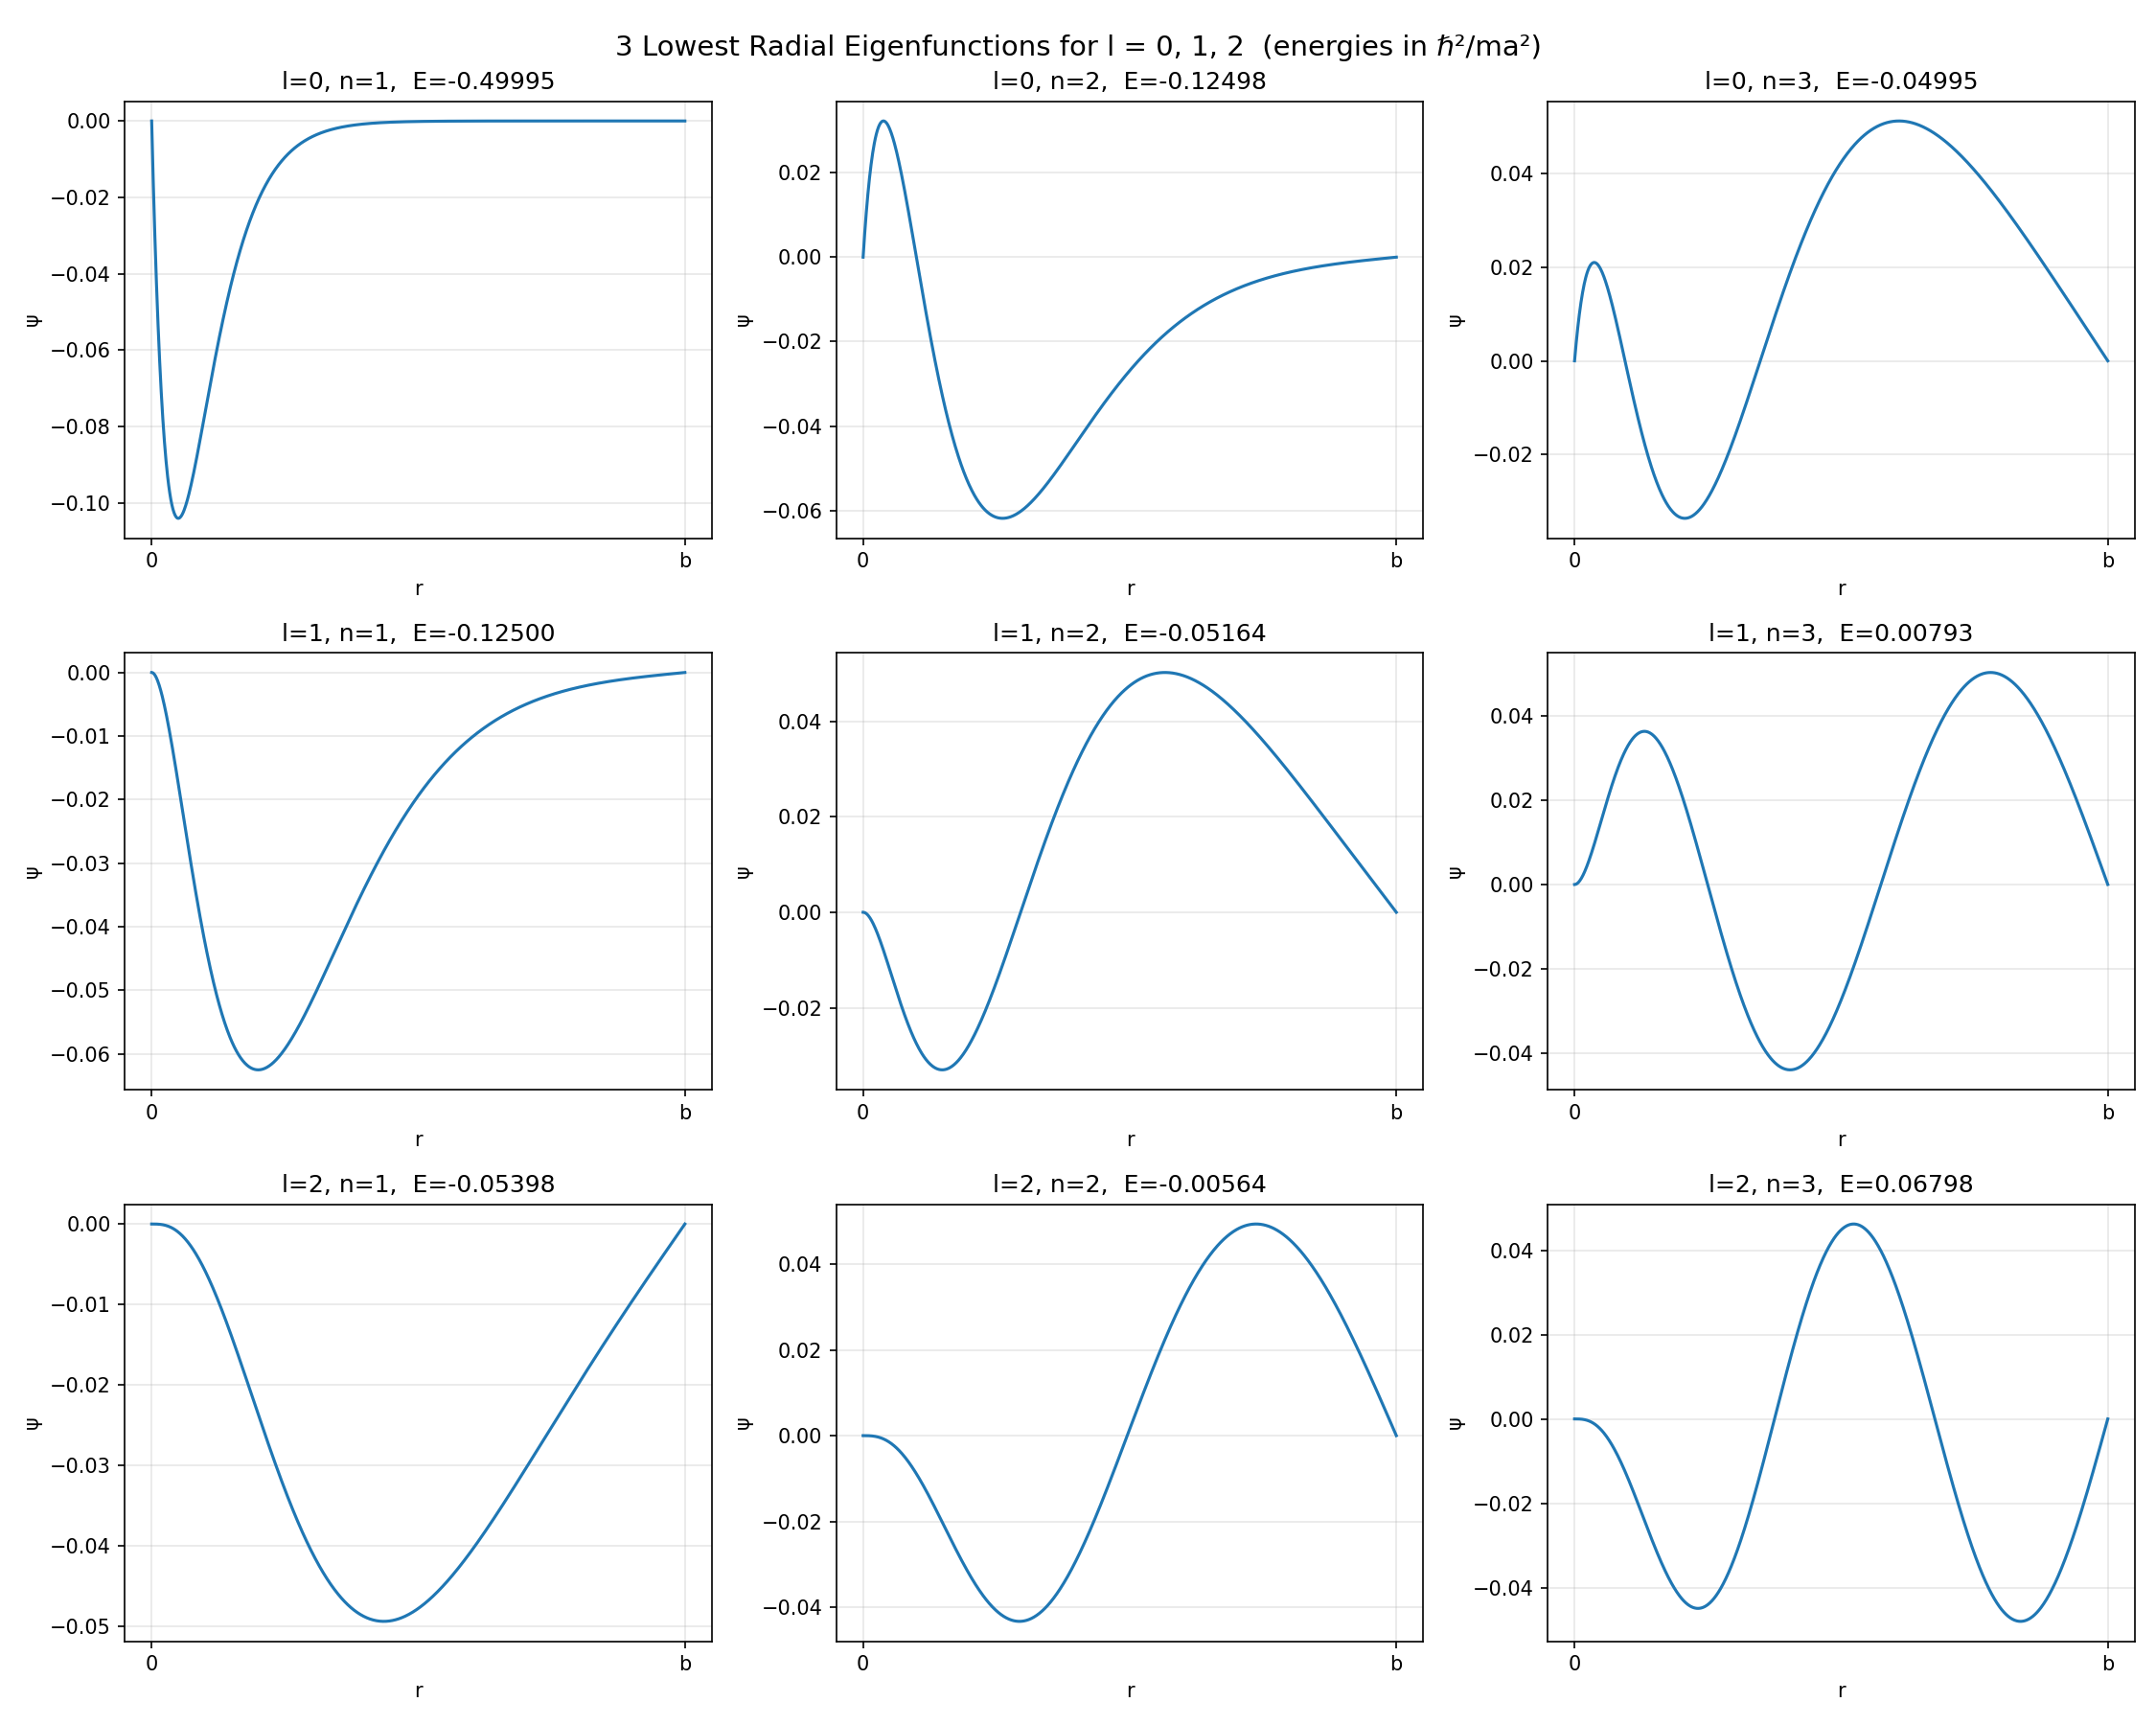
\includegraphics[valign=t,width=\textwidth]{fig/prob4.68_eigenfunctions.png}
     By eq 4.70, the lowest three energies in $\frac{\hbar^2}{ma^2}$ unit are $-0.5,\; -0.125, \;-0.0556.$
 \end{enumerate}
 \subsection*{Sol. 69}
 For $l=0,$ the lowest three $n$s are 
 $1.0000,$ $2.0000,$ $3.0000$.
 
 For $l=1,$ the lowest three $n$s are 
 $2.0000,$ $3.0000,$ $4.0000$.

 For $l=2,$ the lowest three $n$s are 
 $3.0000,$ $4.0000,$ $5.0000$.

 \subsection*{Sol. 70}
 \begin{enumerate}
     \item 
     All got spin up in the first experiment. If that particle is in the z direction group, it measured spin up for sure. If it is in the x direction group, since it is selected as spin up, the  measurement first time is spin up for sure.
     \item 
     Equation 4.155 gives 
     $$
     \chi_+^{(r)}
     =
     \begin{pmatrix}
         \cos\theta/2\\
         e^{i\phi}
         \sin\theta/2
     \end{pmatrix},\;
     \chi_-^{(r)}
     =
     \begin{pmatrix}
         e^{-i\phi}
         \sin\theta\\
         -\cos\theta/2
     \end{pmatrix}
     $$
     Note that, by choosing $\bm a$ as the z axis, the probability of measuring spin up along $\bm b$ for a spin up $\bm a$ particle is 
     \begin{align*}
         &\bigg|
         \begin{pmatrix}
         1 && 0
     \end{pmatrix}
         \begin{pmatrix}
             \cos\theta_{ab}/2\\
             e^{i\phi}
             \sin\theta_{ab}/2
         \end{pmatrix}
         \bigg|^2\\
         =&
         \cos^2\frac{\theta_{ab}}{2}
     \end{align*}
     We can get all four probabilities 
     $$
     P_{++}
     =
    \cos^2\frac{\theta_{bc}}{2} \cos^2\frac{\theta_{ab}}{2}
     $$
     $$
     P_{+-}
     =
    \sin^2\frac{\theta_{bc}}{2} \cos^2\frac{\theta_{ab}}{2}
     $$
     $$
     P_{-+}
     =
    \sin^2\frac{\theta_{bc}}{2} \sin^2\frac{\theta_{ab}}{2}
     $$
     $$
     P_{--}
     =
    \cos^2\frac{\theta_{bc}}{2} \sin^2\frac{\theta_{ab}}{2}
     $$
     \begin{align*}
         P_{\text{first up}|\text{second up}}
         =&\frac{\cos^2\frac{\theta_{bc}}{2} \cos^2\frac{\theta_{ab}}{2}}
         {\sin^2\frac{\theta_{bc}}{2} \sin^2\frac{\theta_{ab}}{2}+\cos^2\frac{\theta_{bc}}{2} \cos^2\frac{\theta_{ab}}{2}}\\
         =&(1+\tan^2\frac{\theta_{ab}}{2}\tan^2\frac{\theta_{bc}}{2})^{-1}.
     \end{align*}
     
 \end{enumerate}
 \subsection*{Sol. 71}
 \begin{enumerate}
     \item 
     $$
     \psi_{21-1}(r,\theta,\phi)
     =\frac{1}{2\sqrt{6}}a^{-3/2}\frac{r}{a}\exp(-\frac{r}{2a})\sqrt{\frac{3}{8\pi}}\sin\theta e^{-i\phi}
     $$
     $$
     \psi_{210}(r,\theta,\phi)
     =\frac{1}{2\sqrt{6}}a^{-3/2}\frac{r}{a}\exp(-\frac{r}{2a})\sqrt{\frac{3}{4\pi}}\cos\theta
     $$
     $$
     \psi_{211}(r,\theta,\phi)
     =-\frac{1}{2\sqrt{6}}a^{-3/2}\frac{r}{a}\exp(-\frac{r}{2a})\sqrt{\frac{3}{8\pi}}\sin\theta e^{i\phi}
     $$

     \begin{align*}
         \psi_{2p_x}(r,\theta,\phi)
         =\frac{1}{\sqrt{32\pi a^3}}\frac{r\sin\theta\cos\phi}{a}\exp(-\frac{r}{2a})
         =
         \frac{1}{\sqrt{2}}\psi_{21-1}(r,\theta,\phi)
         -\frac{1}{\sqrt{2}}\psi_{211}(r,\theta,\phi)
     \end{align*}
     \begin{align*}
         \psi_{2p_y}(r,\theta,\phi)
         =\frac{1}{\sqrt{32\pi a^3}}\frac{r\sin\theta\sin\phi}{a}\exp(-\frac{r}{2a})
         =
         \frac{i}{\sqrt{2}}\psi_{21-1}(r,\theta,\phi)
         +\frac{i}{\sqrt{2}}\psi_{211}(r,\theta,\phi)
     \end{align*}
     \begin{align*}
         \psi_{2p_z}(r,\theta,\phi)
         =\frac{1}{\sqrt{32\pi a^3}}\frac{r\cos\theta}{a}\exp(-\frac{r}{2a})
         =\psi_{210}(r,\theta,\phi)
     \end{align*}
     \item 
     \begin{align*}
         L_x\psi_{2p_x}
         =&
         -i\hbar(-\sin\phi\frac{\partial}{\partial\theta}-\cos\phi\cot\theta\frac{\partial}{\partial\phi})
         \frac{1}{\sqrt{32\pi a^3}}\frac{r\sin\theta\cos\phi}{a}\exp(-\frac{r}{2a})\\
         =&
         \frac{-i\hbar}{\sqrt{32\pi a^3}}\frac{r}{a}\exp(-\frac{r}{2a})
         (-\sin\phi\cos\theta\cos\phi + \cos\phi\cot\theta\sin\theta\sin\phi)\\
         =&0
     \end{align*}
     \begin{align*}
         L_y\psi_{2p_y}
         =&
         -i\hbar(\cos\phi\frac{\partial}{\partial\theta}-\sin\phi\cot\theta\frac{\partial}{\partial\phi})
         \frac{1}{\sqrt{32\pi a^3}}\frac{r\sin\theta\sin\phi}{a}\exp(-\frac{r}{2a})\\
         =&-i\hbar\frac{1}{\sqrt{32\pi a^3}}\frac{r}{a}\exp(-\frac{r}{2a})
         (\cos\phi\cos\theta\sin\phi-\sin\phi\cot\theta\sin\theta\cos\phi)\\
         =&0
     \end{align*}
     \begin{align*}
         L_z\psi_{2p_z}=&
         -i\hbar\frac{\partial}{\partial\phi}
         \frac{1}{\sqrt{32\pi a^3}}\frac{r\cos\theta}{a}\exp(-\frac{r}{2a})\\
         =&0
     \end{align*}
     \item 
     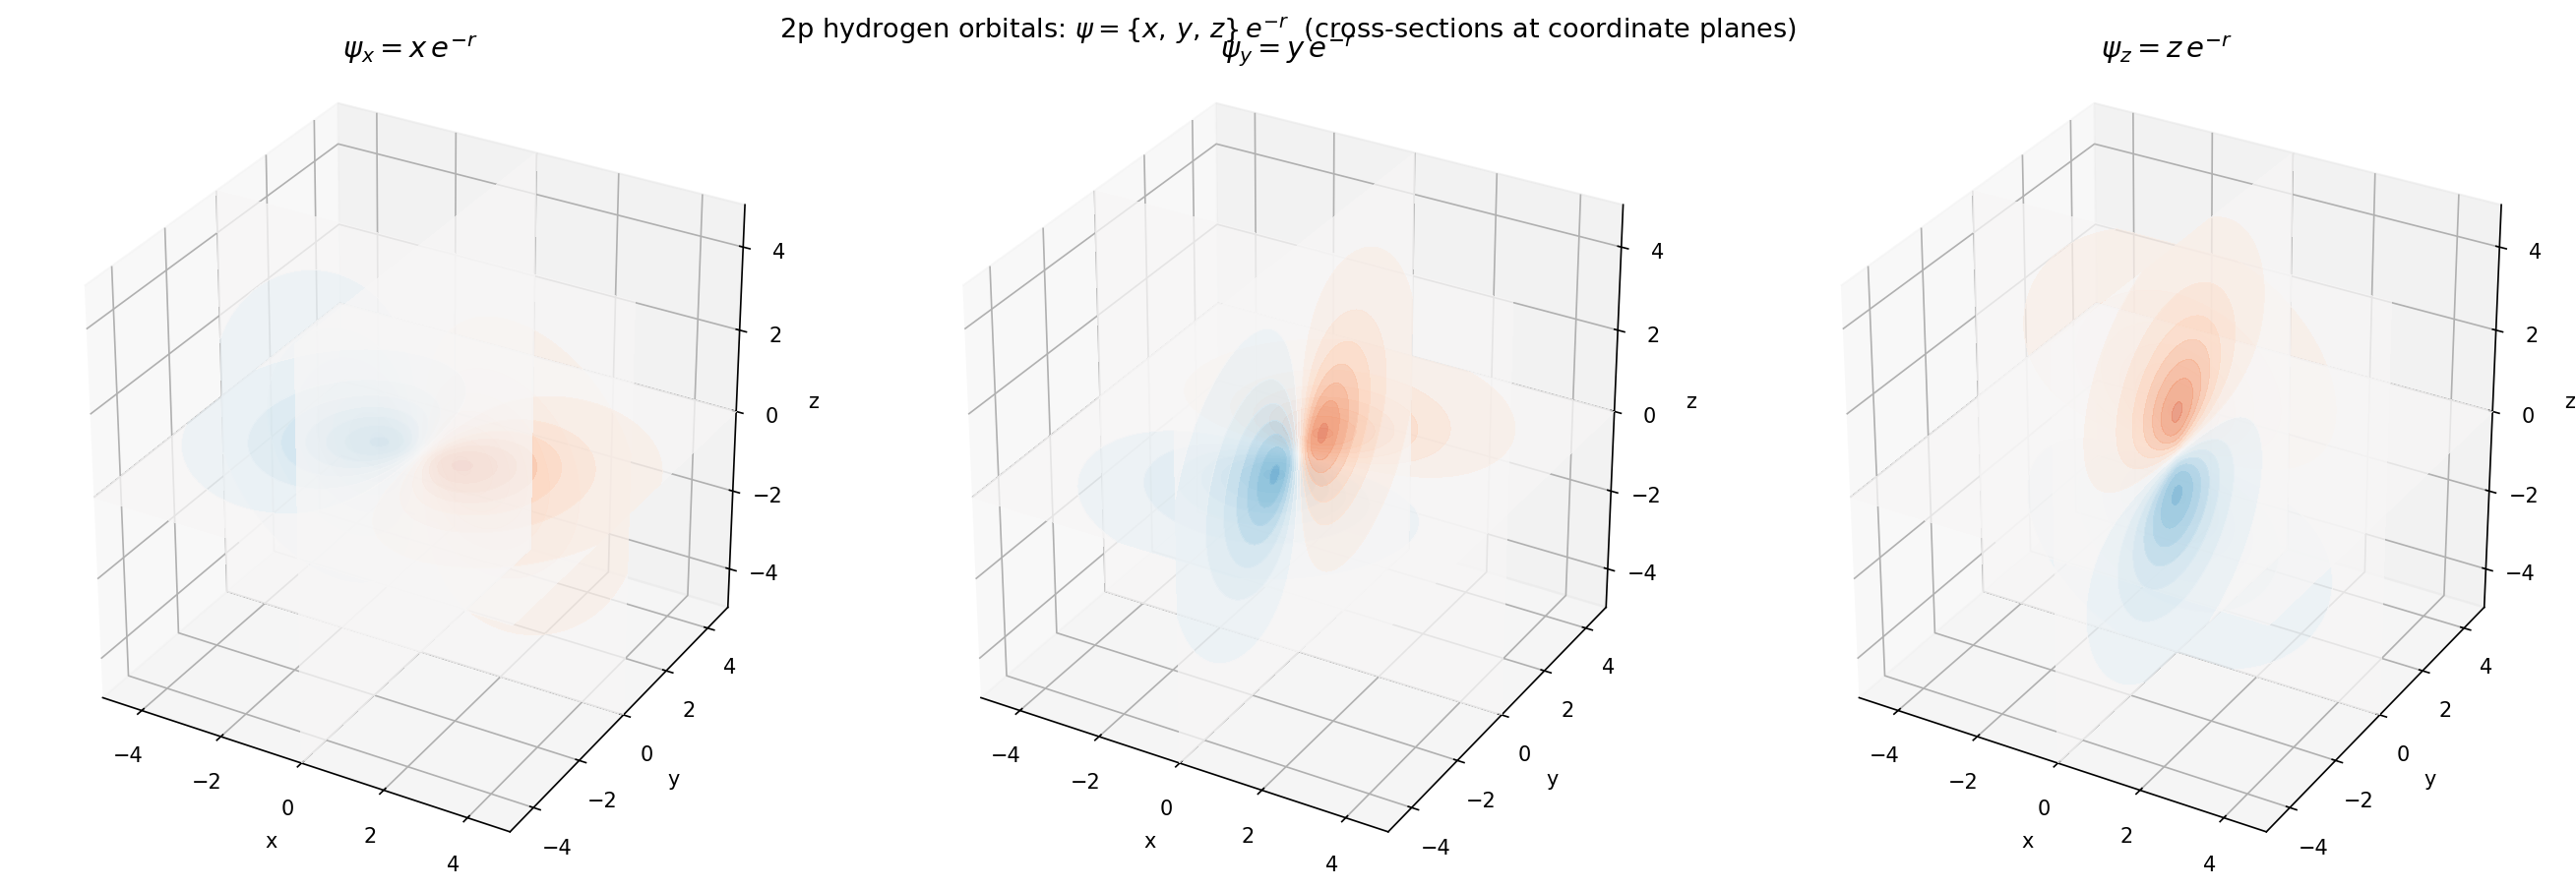
\includegraphics[valign=t,width=\textwidth]{fig/prob4.71_orbitals.png}
 \end{enumerate}
 \subsection*{Sol. 72}
 \begin{enumerate}
     \item 
     \begin{align*}
         \nabla\times\bm A =&
         \nabla\times(-\frac{1}{2}\bm r \times \bm B_0)\\
         = &
         -\frac{1}{2}\nabla\times
         ((yB_{0z}-zB_{0y})\hat i+
         (zB_{0x}-xB_{0y})\hat j +
         (xB_{0y}-yB_{0x})\hat k)\\
         =&
         -\frac{1}{2}
         ((-B_{0x}-B_{0x})\hat i +
         (-B_{0y}-B_{0y})\hat j +
         (-B_{0z}-B_{0z})\hat k)\\
         =&\bm B_0
     \end{align*}
     \item By equation 4.199 and equation 4.157
     \begin{align*}
         H =& \frac{1}{2m}
         (p^2+q^2\frac{1}{4}(\bm r\times \bm B_0)^2
         -i\hbar q(\bm r\times \bm B_0)\cdot\nabla)-\bm B_0\cdot(\gamma\bm S)+q\varphi
     \end{align*}
     \begin{align*}
         (\bm r\times \bm B_0)^2
         =r^2B_0^2-(\bm r\cdot \bm B_0)^2
     \end{align*}
     \begin{align*}
         -i\hbar q(\bm r\times \bm B_0)\cdot \nabla\psi
         =&i\hbar q\bm B_0\cdot (\bm r\times \nabla\psi)\\
         =&-q\bm B_0\cdot \bm L\psi,
     \end{align*}
     so 
     \begin{align*}
         H = 
         \frac{p^2}{2m}
         +q\varphi 
         -\bm B_0\cdot
         (\gamma_0\bm L+\gamma \bm S)
         +
         \frac{q^2}{8m}
         (r^2B_0^2-(\bm r\cdot \bm B_0)^2).
     \end{align*}
     
 \end{enumerate}
 \subsection*{Sol. 73}
 $$
 \bm B = -\alpha x\hat i + (B_0+\alpha z)\hat k 
 $$
 \begin{align*}
     \frac{d^2}{dt^2}
     \langle z\rangle
     =&
     \frac{i}{\hbar}
     \frac{d}{dt}
     \langle[H,z]\rangle\\
     =&\frac{i}{\hbar}
     \frac{i}{\hbar}
     \langle[H,[H,z]]\rangle\\
     =&-\frac{1}{\hbar^2}
     \langle[\frac{p^2}{2m}-\gamma\bm B\cdot \bm S, -2i\hbar p_z]\rangle\\
     =&-\frac{1}{\hbar^2}
     \langle-\gamma \alpha z S_z, \frac{-2i\hbar}{2m} p_z\rangle\\
     =&\frac{1}{m}\gamma\alpha\langle S_z\rangle.
 \end{align*}

 \subsection*{Sol. 74}
 \begin{enumerate}
     \item 
     \begin{align*}
         (\frac{p^2}{2m}-\gamma\bm B\cdot\bm S)
         (\Psi_+\chi_++\Psi_-\chi_-)
         =i\hbar\frac{\partial}{\partial t}
         (\Psi_+\chi_++\Psi_-\chi_-)
     \end{align*}
     \begin{align*}
         &(-\frac{\hbar^2}{2m}\nabla^2
         -\gamma(-\alpha xS_x+(B_0+\alpha z)S_z))
         (\Psi_+\chi_++\Psi_-\chi_-)\\
         =&
         -\frac{\hbar^2}{2m}\nabla^2\Psi_+\chi_+
         -\frac{\hbar^2}{2m}\nabla^2\Psi_-\chi_-
         +\gamma\alpha x\Psi_+\frac{\hbar}{2}\chi_-\\
         &+\gamma\alpha x\Psi_-\frac{\hbar}{2}\chi_+
         -\gamma(B_0+\alpha z)\Psi_+\frac{\hbar}{2}\chi_+
         +\gamma(B_0+\alpha z)\Psi_-\frac{\hbar}{2}\chi_-
     \end{align*}
     We therefore have two coupled equations
     \begin{align*}
         -\frac{\hbar^2}{2m}\nabla^2\Psi_+
         +\frac{\hbar}{2}\gamma\alpha x\Psi_- 
         -\frac{\hbar}{2}\gamma (B_0+\alpha z)\Psi_+ = 
         i\hbar \frac{\partial}{\partial t}\Psi_+
     \end{align*}
     \begin{align*}
         -\frac{\hbar^2}{2m}\nabla^2\Psi_-
         +\frac{\hbar}{2}\gamma\alpha x\Psi_+ 
         +\frac{\hbar}{2}\gamma (B_0+\alpha z)\Psi_- = 
         i\hbar \frac{\partial}{\partial t}\Psi_-
     \end{align*}
     \item 
     \begin{align*}
         -\frac{\hbar^2}{2m}\nabla^2
         e^{i\gamma B_0t/2}\tilde\Psi_+
         +\frac{\hbar}{2}\gamma\alpha x
         e^{-i\gamma B_0t/2}\tilde\Psi_-
         -\frac{\hbar}{2}\gamma (B_0+\alpha z)
         e^{i\gamma B_0t/2}\tilde\Psi_+= 
         i\hbar \frac{\partial}{\partial t}
         e^{i\gamma B_0t/2}\tilde\Psi_+
     \end{align*}
     \begin{align*}
         -\frac{\hbar^2}{2m}\nabla^2
         \tilde\Psi_+
         +\frac{\hbar}{2}\gamma\alpha x
         e^{-i\gamma B_0t}\tilde\Psi_-
         -\frac{\hbar}{2}\gamma \alpha z
         \tilde\Psi_+= 
         i\hbar \frac{\partial}{\partial t}
         \tilde\Psi_+
     \end{align*}
     \begin{align*}
         -\frac{\hbar^2}{2m}\nabla^2
         e^{-i\gamma B_0t/2}\tilde\Psi_-
         +\frac{\hbar}{2}\gamma\alpha x
         e^{i\gamma B_0t/2}\tilde\Psi_+ 
         +\frac{\hbar}{2}\gamma (B_0+\alpha z)
         e^{-i\gamma B_0t/2}\tilde\Psi_- = 
         i\hbar \frac{\partial}{\partial t}
         e^{-i\gamma B_0t/2}\tilde\Psi_-
     \end{align*}
     \begin{align*}
         -\frac{\hbar^2}{2m}\nabla^2
         \tilde\Psi_-
         +\frac{\hbar}{2}\gamma\alpha x
         e^{i\gamma B_0t}\tilde\Psi_+ 
         +\frac{\hbar}{2}\gamma \alpha z
         \tilde\Psi_- = 
         i\hbar \frac{\partial}{\partial t}
         \tilde\Psi_-
     \end{align*}
     \item 
     \begin{align*}
         -\frac{\hbar^2}{2m}
         \nabla^2\tilde\Psi_{\pm}
         \mp\frac{\hbar}{2}\gamma\alpha z\tilde\Psi_{\pm}
         =i\hbar\frac{\partial}{\partial t}\tilde\Psi_{\pm}
     \end{align*}

        By Ehrenfest's Theorem, the expectation value of the z component of $\tilde\Psi_+$ goes up, and the expectation value of the z component of $\tilde\Psi_-$ goes down, splitting both spatial wave functions apart. Once it hits the screen,
        the spin state collapses, and the difference in the z component of both states makes the two stripes.
 \end{enumerate}

 \subsection*{Sol. 75}
 \begin{align*}
     H\Psi(\phi,t)
    =& \frac{1}{2m}
    \left[
    -\frac{\hbar^2}{b^2}\frac{d^2}{d\phi^2}
    +\left(
    \frac{q\Phi}{2\pi b}
    \right)^2
    +
    i\frac{\hbar q\Phi}{\pi b^2}
    \frac{d}{d\phi}
    \right]
    \frac{1}{\sqrt{2\pi}}
    e^{in\phi}
    e^{-if(t)}\\
    =&\frac{1}{2m}
    \left[
    \frac{\hbar^2}{b^2}n^2
    +\left(
    \frac{q\Phi}{2\pi b}
    \right)^2
    -
    \frac{\hbar q\Phi n}{\pi b^2}
    \right]
    \frac{1}{\sqrt{2\pi}}
    e^{in\phi}
    e^{-if(t)}\\
    =&\frac{1}{\sqrt{2\pi}}
     e^{in\phi}
     e^{-if(t)}
     \frac{\hbar^2}{2mb^2}
     \left(
    n- \frac{q\Phi}{2\pi\hbar}
     \right)^2
 \end{align*}
 \begin{align*}
     i\hbar\frac{\partial}{\partial t}
     \frac{1}{\sqrt{2\pi}}
     e^{in\phi}
     e^{-if(t)}
     =& 
     i\hbar
     \frac{1}{\sqrt{2\pi}}
     e^{in\phi}
     e^{-if(t)}
     (-if'(t))\\
     =&
     \frac{1}{\sqrt{2\pi}}
     e^{in\phi}
     e^{-if(t)}
     \frac{\hbar^2}{2mb^2}
     \left(
    n- \frac{q\Phi}{2\pi\hbar}
     \right)^2
 \end{align*}

 \subsection*{Sol. 76}
 \begin{enumerate}
     \item 
     \begin{align*}
        \mathcal{E}
         =&-\frac{d\Phi}{dt}
         =2\pi Fb
     \end{align*}
     
     $$
     W = \int qF b\omega dt
     =-\int \frac{q\omega}{2\pi} d\Phi
     $$
     $$
     \frac{dW}{d\Phi}
     =-\frac{q\omega}{2\pi}.
     $$
     \item 
     \begin{align*}
         \bm r\times (\bm p - q\bm A)
         \frac{1}{\sqrt{2\pi}}
         \exp\left(
         in\phi
         \right)
         =&
         \bm r\times 
         (\frac{1}{\sqrt{2\pi}}\frac{1}{b}
         \hbar n
         \exp\left(
         in\phi
         \right)\hat\phi -
         \frac{1}{\sqrt{2\pi}}
         \frac{q\Phi}{2\pi b}
         \exp\left(
         in\phi
         \right)\hat\phi
         )
     \end{align*}
     The z component is 
     \begin{align*}
         \frac{1}{\sqrt{2\pi}}
         \hbar n
         \exp\left(
         in\phi
         \right) -
         \frac{1}{\sqrt{2\pi}}
         \frac{q\Phi}{2\pi}
         \exp\left(
         i n\phi
         \right),
     \end{align*}
     so the $z$ component of the mechanical angular momentum is 
     $\hbar n-\frac{q\Phi}{2\pi}.$
     \item 
     $$
     L = mb^2\omega,
     $$
     so
     \begin{align*}
         \frac{dE_n}{d\Phi}
         =&
         \frac{\hbar^2}{2mb^2}
         2\left(
         n-\frac{q\Phi}{2\pi\hbar}
         \right)
         (-\frac{q}{2\pi\hbar})\\
         =&
         -
         \frac{\hbar^2}{2mb^2}
         2\frac{mb^2\omega}{\hbar}
         \frac{q}{2\pi\hbar}\\
         =&-
         \frac{q\omega}{2\pi}
         =\frac{dW}{d\Phi}
     \end{align*}
 \end{enumerate}